% ------------------------------------------------------------------
% CAPSTONE SOFTWARE REQUIREMENTS SPECIFICATION (SRS)
%
% Based on the capTemplate IEEE SRS template, which is inspired by
% ISO/IEC/IEEE 29148 and simplified for a senior capstone project.
% Changes to the template are listed in Section 1 ("Template Changes").
%
% Traceability conventions (keep these consistent when editing):
%   - Every FR ends with "Supports:" (the NFRs it helps satisfy).
%   - Every NFR ends with "Satisfied by:" (the FRs that realize it).
%   - Every SR ends with "Refined by:" (the UCs, FRs and NFRs that refine
%     it); every UC, FR and NFR lists the SRs it traces to.
%   - The matrices in Section 10 summarize these lines; update both.
% ------------------------------------------------------------------

\documentclass[12pt]{article}

\usepackage{lmodern}
\usepackage[T1]{fontenc}
\usepackage{amsmath, mathtools}
\usepackage{amsfonts}
\usepackage{amssymb}
\usepackage{graphicx}
\usepackage{xr}
\usepackage{hyperref}
\usepackage{longtable}
\usepackage{xfrac}
\usepackage{tabularx}
\usepackage{float}
\usepackage{siunitx}
\usepackage{booktabs}
\usepackage{caption}
\usepackage{pdflscape}
\usepackage{afterpage}
\usepackage{array}
\usepackage{enumitem}
\newcolumntype{L}[1]{>{\raggedright\arraybackslash}p{#1}}
\usepackage{tikz}
\usetikzlibrary{arrows.meta, positioning, shapes.geometric, fit,
  backgrounds}

\usepackage[round]{natbib}

\hypersetup{
    bookmarks=true,         % show bookmarks bar?
      colorlinks=true,       % false: boxed links; true: colored links
    linkcolor=red,          % color of internal links (change box color with linkbordercolor)
    citecolor=green,        % color of links to bibliography
    filecolor=magenta,      % color of file links
    urlcolor=cyan           % color of external links
}

\input{../Comments.text}
\input{../Common.text}

% Used so that cross-references have a meaningful prefix

\newcounter{srnum} %Stakeholder Requirement (SR) Number
\newcommand{\srthesrnum}{SR\thesrnum}
\newcommand{\srref}[1]{\hyperref[#1]{SR\ref*{#1}}}

\newcounter{ucnum} %Use Case (UC) Number
\newcommand{\uctheucnum}{UC\theucnum}
\newcommand{\ucref}[1]{\hyperref[#1]{UC\ref*{#1}}}

\newcounter{reqnum} %Functional Requirement (FR) Number
\newcommand{\rthereqnum}{FR\thereqnum}
\newcommand{\rref}[1]{\hyperref[#1]{FR\ref*{#1}}}

\newcounter{nfrnum} %Non-Functional Requirement (NFR) Number
\newcommand{\rthenfrnum}{NFR\thenfrnum}
\newcommand{\nfrref}[1]{\hyperref[#1]{NFR\ref*{#1}}}

\newcounter{lcnum} %Likely Change (LC) Number
\newcommand{\lthelcnum}{LC\thelcnum}
\newcommand{\lcref}[1]{\hyperref[#1]{LC\ref*{#1}}}

\newcounter{ulcnum} %Unlikely Change (ULC) Number
\newcommand{\ulcref}[1]{\hyperref[#1]{ULC\ref*{#1}}}

\newcounter{asnum} %Assumption (A) Number
\newcommand{\asref}[1]{\hyperref[#1]{A\ref*{#1}}}

\newcounter{cnum} %System Constraint (C) Number
\newcommand{\cref}[1]{\hyperref[#1]{C\ref*{#1}}}

\newcounter{elnum} %Elicitation Source (E) Number
\newcommand{\eref}[1]{\hyperref[#1]{E\ref*{#1}}}

\newcounter{ratnum} %Rationale (R) Number
\newcommand{\ratref}[1]{\hyperref[#1]{R\ref*{#1}}}

% Item labels that define a numbered, referenceable entity
\newcommand{\srdef}[1]{\refstepcounter{srnum}\label{#1}\textbf{SR\thesrnum:}}
\newcommand{\frdef}[1]{\refstepcounter{reqnum}\label{#1}\textbf{FR\thereqnum:}}
\newcommand{\nfrdef}[1]{\refstepcounter{nfrnum}\label{#1}\textbf{NFR\thenfrnum:}}
\newcommand{\lcdef}[1]{\refstepcounter{lcnum}\label{#1}\textbf{LC\thelcnum:}}
\newcommand{\ulcdef}[1]{\refstepcounter{ulcnum}\label{#1}\textbf{ULC\theulcnum:}}
\newcommand{\asdef}[1]{\refstepcounter{asnum}\label{#1}\textbf{A\theasnum:}}
\newcommand{\cdef}[1]{\refstepcounter{cnum}\label{#1}\textbf{C\thecnum:}}
\newcommand{\ratdef}[1]{\refstepcounter{ratnum}\label{#1}\textbf{R\theratnum:}}

% Symbolic constants (values are given in Appendix C, Table
% tab:Constants). The macro cst prints a constant's name and links to its
% definition.
\newcommand{\cst}[1]{\hyperref[const:#1]{\texttt{\detokenize{#1}}}}
\newcommand{\cstdef}[1]{\leavevmode\phantomsection\label{const:#1}\texttt{\detokenize{#1}}}

% Glossary terms: \term{Key}{Text} links Text to the definition of Key
\newcommand{\term}[2]{\hyperref[term:#1]{#2}}
\newcommand{\termdef}[2]{\leavevmode\phantomsection\label{term:#1}#2}

% Requirement attribute lines
\newcommand{\attr}[2]{\par\noindent\hspace*{0pt}\textit{#1:} #2}

% Links to the other project documents
\newcommand{\repourl}{https://github.com/team-hindsight/ophthamology-game}
\newcommand{\vnvplan}{\href{\repourl/blob/main/pdfs/VnVPlan/VnVPlan.pdf}{Verification and Validation (VnV) Plan}}
\newcommand{\vnvplanshort}{\href{\repourl/blob/main/pdfs/VnVPlan/VnVPlan.pdf}{VnV Plan}}
\newcommand{\hadoc}{\href{\repourl/blob/main/pdfs/HazardAnalysis/HazardAnalysis.pdf}{Hazard Analysis}}
\newcommand{\psdoc}{\href{\repourl/blob/main/pdfs/ProblemStatementAndGoals/ProblemStatement.pdf}{Problem Statement and Goals}}
\newcommand{\dpdoc}{\href{\repourl/blob/main/pdfs/DevelopmentPlan/DevelopmentPlan.pdf}{Development Plan}}
\newcommand{\issue}[1]{\href{\repourl/issues/#1}{\##1}}

% Math helpers for the formal specification (Section 6.9)
\newcommand{\Bool}{\mathbb{B}}
\newcommand{\Nat}{\mathbb{N}}
\newcommand{\Realnn}{\mathbb{R}_{\geq 0}}
\newcommand{\sm}[1]{\mathit{#1}}
\newcommand{\ev}[1]{\mathsf{#1}}

\setlist[itemize]{topsep=2pt, itemsep=2pt}
\setlength{\LTpre}{6pt}
\setlength{\LTpost}{6pt}
% Long constant names cannot be hyphenated; allow extra inter-word space
% instead of overfull lines.
\setlength{\emergencystretch}{3em}

\usepackage{fullpage}

\begin{document}

\title{Software Requirements Specification for \progname: An Ophthalmology
Preparation Game for Children}
\author{\authname}
\date{\today}

\pagenumbering{roman}

\maketitle

~\newpage

\tableofcontents

\listoffigures

\listoftables

~\newpage

\section*{Revision History}

\begin{tabularx}{\textwidth}{p{3cm}p{2cm}X}
\toprule {\bf Date} & {\bf Version} & {\bf Notes}\\
\midrule
2026-10-07 & 0.1 & First complete draft of Revision 0: all template
sections completed; formal specification of the activity rules; safety and
security requirements added from the \hadoc{}.\\
\bottomrule
\end{tabularx}

\newpage

\pagenumbering{arabic}

% ==============================================================
\section{Introduction}
% ==============================================================

This document is the Software Requirements Specification (SRS) for
\progname{}, a mobile game that prepares children aged \cst{MIN_AGE} to
\cst{MAX_AGE} years for paediatric ophthalmology appointments. It records
\emph{what} \progname{} must do and how well it must do it, so that a
designer outside the team could design, build and test the product from this
document alone. Section~\ref{sec_Purpose} states the purpose of the system,
Section~\ref{sec_Scope} its scope, Section~\ref{sec_Stakeholders} its
stakeholders, and Section~\ref{sec_Definitions} the terms used throughout.

The structure follows the IEEE SRS template of the course template repository
\citep{SmithCapTemplate}, which is based on ISO/IEC/IEEE 29148
\citep{ISOIECIEEE29148_2018}. ISO (International Organization for
Standardization), IEC (International Electrotechnical Commission) and IEEE
(Institute of Electrical and Electronics Engineers) jointly publish this
standard, which justifies the structure of the document, while ISO/IEC/IEEE
15288 \citep{ISOIECIEEE15288_2023} gives the life-cycle context in which the
requirements are used. The document is a reference: it is generally read in
whichever order the reader needs, and Section~\ref{sec_Conventions} explains
how to navigate it.

\subsection*{Template Changes}
\label{sec_TemplateChanges}

All section headings of the template are kept, in the template's order. The
following additions were made so that the document covers everything the
course rubric asks for. No template section was removed or renamed.

\begin{itemize}
\item Section~\ref{sec_Conventions} (Notation and Conventions) was added to
  Section~1 to define requirement identifiers, symbolic constants and the
  mathematical notation.
\item Section~\ref{sec_Assumptions} (Assumptions) was added to Section~2 to
  state the assumptions explicitly. Section~\ref{sec_SystemContext} gained a
  table of system inputs and outputs and a table of functional areas.
\item Section~\ref{sec_StakeholderReqs} adds a ``Source'' line to each
  stakeholder requirement, tracing it to the elicitation records in
  Appendix~\ref{sec_AppendixA}.
\item Sections~\ref{sec_FR} and \ref{sec_NFR} group the requirements into
  subsections. Section~\ref{sec_FR} adds subsections for undesired event
  handling (Section~\ref{sec_UndesiredEvents}) and for the formal
  specification of the most critical behaviour
  (Section~\ref{sec_FormalSpec}).
\item The template's Development Team stakeholder is replaced by future
  maintainers, because team members are not stakeholders of their own
  product.
\item Unlikely changes use the prefix ULC instead of LC, so that every
  identifier in the document is unique.
\item Section~\ref{sec_AI} is kept but marked ``not applicable'', with the
  reason and the conditions under which it would apply.
\end{itemize}

\subsection{Purpose}
\label{sec_Purpose}

\progname{} is intended to solve the problem of children arriving at eye
appointments without knowing what will happen to them. Paediatric
ophthalmology appointments involve unfamiliar equipment, bright lights, eye
drops that sting, and long periods of keeping still. Children who do not know
what to expect are often anxious, and anxious children cooperate less: in a
study of 298 children receiving eye drops, 26\% showed significant distress
before the drops, and uncooperative children were more anxious and took
longer to examine \citep{ChiaEtAl2015}. Preparing children for medical
procedures in advance is known to reduce anxiety and improve outcomes in
other paediatric settings \citep{KainEtAl2007}.

The purpose of \progname{} is to let a child, at home or in the waiting room,
learn what happens during each common eye-clinic procedure and practise the
behaviour the clinician will ask for, so that the child is calmer and more
cooperative during the real examination. The project goals that this purpose
serves are stated in the \psdoc{} document and summarized in
Section~\ref{sec_ProductVision}.

\subsection{Scope}
\label{sec_Scope}

\progname{} is a free, offline game for phones and tablets. A child picks a
clinic procedure (for example, ``Eye Drops''), follows a friendly eye doctor
character through a narrated, step-by-step walkthrough of that procedure,
practises the required behaviour through simple touch activities, and earns a
sticker. A caregiver (a parent or other adult responsible for the child) can
choose which procedures the upcoming visit will include, read a description
of each procedure, adjust sound and caption settings, and view a record of
what the child has practised. The expected benefits are lower anxiety,
better cooperation and shorter, less difficult examinations
(Section~\ref{sec_ProductVision}).

Table~\ref{tab:ProcedureCatalogue} lists the procedures in scope. The list
comes from the clinic observation visit (\eref{E_ClinicVisit}) and the
supervisor's project description (\eref{E_ProjectDescription}). The order in
which their content is produced is given in Appendix~\ref{sec_AppendixB}.
Every procedure is presented as a preparation walkthrough; none of them
measures anything about the child.

\begin{longtable}{L{0.20\textwidth} L{0.42\textwidth} L{0.28\textwidth}}
\caption{Procedure Catalogue: clinic procedures in scope}
\label{tab:ProcedureCatalogue}\\
\toprule
\textbf{Procedure} & \textbf{What the child experiences} &
\textbf{Behaviour practised}\\
\midrule
\endfirsthead
\toprule
\textbf{Procedure} & \textbf{What the child experiences} &
\textbf{Behaviour practised}\\
\midrule
\endhead
Eye Drops (dilation) & Head tilted back; drops feel cold and may sting or
burn briefly; vision is blurry and bright for a few hours; a wait of about 20
minutes while the drops work. & Head back, eyes open, then blinking.\\
Vision Test & Naming pictures or letters on a chart from a chair, with one eye
covered at a time. & Keeping one eye covered; naming pictures.\\
Slit Lamp Exam & Chin and forehead resting on a large microscope while the
doctor looks through it with a bright light. & Keeping the head still against
the rest.\\
Headlamp Exam & The doctor wears a bright light on the head and looks into the
eye, often after the drops. & Looking where asked despite a bright light.\\
Eye Pressure Check & A small tool gently touches the surface of the eye after
numbing drops. & Keeping eyes open and still.\\
Eye Photos & A camera or scanner takes pictures of the inside of the eye. &
Looking at a target and keeping still.\\
Colour Vision Test & Finding numbers or shapes in coloured dot pictures in a
book. & Pointing to what is seen.\\
Glasses Check & The doctor shines a light through lenses held in front of the
eyes. & Looking at a distant target.\\
Eye Alignment Test & Prisms are held in front of the eyes to measure how the
eyes line up; important before eye-muscle surgery. & Looking at a target while
prisms change.\\
Eye Movement Test & Following the doctor's finger or a toy with the eyes. &
Following a moving target without moving the head.\\
Eye Patch & Wearing a patch over the stronger eye at home. & Wearing the patch
and continuing to play.\\
\bottomrule
\end{longtable}

\noindent \progname{} does \emph{not}:
\begin{itemize}
\item diagnose, screen, measure or monitor vision or any other medical
  condition (the Vision Test walkthrough is practice only);
\item give medical advice, treatment instructions or medication guidance;
\item collect, store or transmit personal or health information about the
  child or family (Section~\ref{sec_Privacy});
\item book or manage appointments, or exchange data with clinic record
  systems beyond reading a non-identifying Visit Code
  (\rref{FR_VisitCode});
\item require an account, an internet connection after installation, or any
  purchase;
\item measure the child's anxiety. Anxiety and cooperation are measured by the
  project's evaluation study with validated instruments outside the product
  (see the \vnvplan{});
\item provide augmented reality, other languages, or clinician-authored
  content in this release. These are documented as likely changes
  (Section~\ref{sec_LikelyChanges}).
\end{itemize}

\subsection{Stakeholders}
\label{sec_Stakeholders}

A stakeholder is anyone with an interest in the system. Stakeholders are
grouped below using the categories of the template. Members of the
development team are not listed, because team members are not stakeholders
of their own product.

\begin{itemize}
\item \textbf{Customer and project sponsor:} the project supervisor, a
  paediatric ophthalmology researcher and clinician who proposed the project
  (\eref{E_ProjectDescription}), and the paediatric eye clinic that will pilot
  the product. They need children who are prepared for their examinations and
  evidence of whether the product works.
\item \textbf{End users:}
  \begin{itemize}
  \item \emph{Children} aged \cst{MIN_AGE} to \cst{MAX_AGE} years with an
    upcoming eye appointment (primary users; Section~\ref{SecUserCharacteristics}).
  \item \emph{Caregivers} (parents, guardians or other adults) who install the
    product, set it up and play alongside younger children.
  \end{itemize}
\item \textbf{Clinicians:} paediatric ophthalmologists, orthoptists and
  ophthalmic technicians who perform the procedures. They benefit from more
  cooperative patients, may tell families which procedures to practise, and
  review the clinical content.
\item \textbf{Child-life specialists and child development experts:} experts
  on how children play and cope with medical care. They review the language
  and imagery and advise on age-appropriate design.
\item \textbf{Regulatory and ethics bodies:} the research ethics board that
  approves studies with children, privacy regulators, and the app store
  operators (Apple and Google), whose policies for children's apps the product
  must satisfy (Section~\ref{sec_Legal}).
\item \textbf{Administrators:} not applicable. \progname{} has no server, no
  accounts and no administration console, so there is no administrator role.
\item \textbf{Future maintainers:} developers who will add procedures and
  maintain the product after the capstone project ends.
\item \textbf{Society:} the public health-care system benefits when
  examinations take less time and fewer children need repeat visits or
  sedation; families with limited resources benefit from a free tool that
  works offline on older devices; and other paediatric services may reuse the
  approach (for example, a family doctor preparing a child for a check-up).
  Society's interests appear as the health, safety, privacy, accessibility and
  cultural requirements in Section~\ref{sec_NFR}.
\end{itemize}

\subsection{Definitions and Acronyms}
\label{sec_Definitions}

Table~\ref{tab:DefinitionsAndAcronyms} defines the terms used in this
document. Terms in \emph{italics} in the requirements are defined here.
Table~\ref{tab:Acronyms} expands every acronym and links to the section
where it is first defined in the text.

\begin{longtable}{L{0.25\textwidth} L{0.65\textwidth}}
\caption{Definitions} \label{tab:DefinitionsAndAcronyms}\\
\toprule
\textbf{Term} & \textbf{Definition}\\
\midrule
\endfirsthead
\toprule
\textbf{Term} & \textbf{Definition}\\
\midrule
\endhead
\termdef{Activity}{Activity} & The interactive part of a step that waits for
the child's input. The activity types are defined in
Section~\ref{sec_FRActivities}.\\
\termdef{AvailabilityState}{Availability State} & One of Available, Completed
or Coming Soon, assigned to each procedure by the function $\sm{avail}$
(Section~\ref{sec_FormalSpec}).\\
\termdef{Caregiver}{Caregiver} & An adult responsible for the child, such as a
parent or guardian, who sets up and supervises the use of \progname{}.\\
\termdef{CaregiverArea}{Caregiver Area} & The part of \progname{} for
caregivers only: notice, procedure guide, settings, Visit Plan, Practice
Summary and progress reset.\\
\termdef{CaregiverCheck}{Caregiver Check} & A short challenge that an adult can
pass and that a child in the target age range is unlikely to pass, which
guards the Caregiver Area (\rref{FR_CaregiverCheck}).\\
\termdef{Child}{Child} & A user aged \cst{MIN_AGE} to \cst{MAX_AGE} years who
plays the walkthroughs.\\
\termdef{Clinician}{Clinician} & An eye-care professional (ophthalmologist,
orthoptist or ophthalmic technician) who performs the procedures.\\
\termdef{Dilation}{Dilation} & Widening of the pupil caused by eye drops so
that the clinician can see the back of the eye.\\
\termdef{Interruption}{Interruption} & In a Hold Still activity, the child
releasing the hold control before the required duration has elapsed
(Section~\ref{sec_FormalSpec}).\\
\termdef{Notice}{Not-Medical-Advice Notice} & A statement that \progname{} is a
preparation aid and does not provide medical advice
(\rref{FR_Notice}).\\
\termdef{PersonalInfo}{Personal Information} & Information about an
identifiable individual, such as name, birth date, photograph, voice, contact
details, location or device identifier, as defined by the Personal
Information Protection and Electronic Documents Act (PIPEDA,
Section~\ref{sec_Legal}).\\
\termdef{PHI}{Personal Health Information} & Personal information about an
individual's health or health care, as defined by the Personal Health
Information Protection Act (PHIPA, Section~\ref{sec_Legal}).\\
\termdef{PracticeSummary}{Practice Summary} & A screen in the Caregiver Area
listing which procedures the child has completed and when
(\rref{FR_PracticeSummary}).\\
\termdef{Procedure}{Procedure} & A clinical procedure from
Table~\ref{tab:ProcedureCatalogue}, and the walkthrough that prepares the
child for it.\\
\termdef{ProcedureCatalogue}{Procedure Catalogue} & The set of procedures
known to a release of \progname{} (Table~\ref{tab:ProcedureCatalogue}).\\
\termdef{ProcedureContent}{Procedure Content} & The data that defines a
walkthrough: its ordered steps, narration, captions, illustrations, sensation
tags and activity parameters (Section~\ref{sec_Data}).\\
\termdef{Progress}{Progress} & The record of completed procedures, their most
recent completion dates and the earned stickers.\\
\termdef{ReferenceDevice}{Reference Device} & A device on which performance and
portability requirements are verified. The list is maintained in the
\vnvplan{} and must satisfy \cst{REFERENCE_DEVICES}.\\
\termdef{SensationTag}{Sensation Tag} & A label on a step stating that the real
procedure involves a physical sensation: cold, sting, bright light, touch,
pressure or blurry vision.\\
\termdef{Step}{Step} & One stage of a walkthrough, consisting of narration and,
optionally, an activity.\\
\termdef{Sticker}{Sticker} & The reward given for the first completion of a
procedure.\\
\termdef{StickerBook}{Sticker Book} & The screen that shows earned stickers.\\
\termdef{VisitCode}{Visit Code} & A short code that a clinic can give a family
to set the Visit Plan; it contains only procedure identifiers
(Section~\ref{sec_DataDictionary}).\\
\termdef{VisitPlan}{Visit Plan} & The set of procedures expected at the
child's next appointment.\\
\termdef{Walkthrough}{Walkthrough} & The ordered sequence of steps that
presents one procedure to the child.\\
\bottomrule
\end{longtable}

\begin{longtable}{L{0.14\textwidth} L{0.56\textwidth} L{0.20\textwidth}}
\caption{Acronyms and abbreviations} \label{tab:Acronyms}\\
\toprule
\textbf{Acronym} & \textbf{Expansion} & \textbf{Defined in}\\
\midrule
\endfirsthead
\toprule
\textbf{Acronym} & \textbf{Expansion} & \textbf{Defined in}\\
\midrule
\endhead
A & Assumption & Section~\ref{sec_Assumptions}\\
AODA & Accessibility for Ontarians with Disabilities Act &
Section~\ref{sec_Legal}\\
AR & Augmented Reality & Section~\ref{sec_ProductVision}\\
C & System Constraint & Section~\ref{sec_Constraints}\\
COPPA & Children's Online Privacy Protection Act (United States) &
Section~\ref{sec_Legal}\\
dBTP & Decibels relative to full scale, True Peak & Section~\ref{sec_LookFeel}\\
E & Elicitation source & Appendix~\ref{sec_AppendixA}\\
FR & Functional Requirement & Section~\ref{sec_Conventions}\\
HA & Hazard Analysis & Section~\ref{sec_Conventions}\\
IEC & International Electrotechnical Commission & Section~1\\
IEEE & Institute of Electrical and Electronics Engineers & Section~1\\
ISO & International Organization for Standardization & Section~1\\
LC & Likely Change & Section~\ref{sec_Conventions}\\
LU & Loudness Unit & Section~\ref{sec_LookFeel}\\
LUFS & Loudness Units relative to Full Scale & Section~\ref{sec_LookFeel}\\
NFR & Nonfunctional Requirement & Section~\ref{sec_Conventions}\\
OCT & Optical Coherence Tomography & Section~\ref{sec_UserCharacteristicsClin}\\
OS & Operating System & Section~\ref{sec_SystemContext}\\
PHI & Personal Health Information & Section~\ref{sec_Legal}\\
PHIPA & Personal Health Information Protection Act (Ontario) &
Section~\ref{sec_Definitions}\\
PIPEDA & Personal Information Protection and Electronic Documents Act (Canada)
& Section~\ref{sec_Definitions}\\
PoC & Proof of Concept & Appendix~\ref{sec_AppendixB}\\
pt & Point, the platform-independent unit of length used by iOS and Android
for interface layout & Section~\ref{sec_LookFeel}\\
R & Rationale & Section~\ref{sec_Rationale}\\
REB & Research Ethics Board & Section~\ref{sec_Constraints}\\
RTM & Requirements Traceability Matrix & Section~\ref{sec_RTM}\\
SaMD & Software as a Medical Device & Section~\ref{sec_Legal}\\
SR & Stakeholder Requirement & Section~\ref{sec_Conventions}\\
SRS & Software Requirements Specification & Section~1\\
SSR & Safety or Security Requirement (\hadoc{}) &
Section~\ref{sec_Conventions}\\
SUS & System Usability Scale & Section~\ref{sec_Usability}\\
UC & Use Case & Section~\ref{sec_Conventions}\\
ULC & Unlikely Change & Section~\ref{sec_Conventions}\\
VnV & Verification and Validation & Section~\ref{sec_Scope}\\
WCAG & Web Content Accessibility Guidelines & Section~\ref{sec_LookFeel}\\
\bottomrule
\end{longtable}

\subsection{Characteristics of Intended Reader}
\label{sec_IntendedReader}

The intended readers are the people who will review, design, implement, test
and maintain \progname{}: the development team, future maintainers, the
teaching assistant and instructor, peer reviewers, and the supervisor. A
reader is expected to have:

\begin{itemize}
\item the knowledge of a fourth-year undergraduate software engineering
  student, including requirements specification, software design and
  testing;
\item working knowledge of discrete mathematics: sets, functions, sequences,
  first-order logic and finite state machines, at the level of a second-year
  university course in discrete mathematics or logic, to read
  Section~\ref{sec_FormalSpec};
\item familiarity with touch-screen mobile applications as a user.
\end{itemize}

\noindent No clinical knowledge is required. The clinical terms used are
defined in Table~\ref{tab:DefinitionsAndAcronyms} and the procedures are
described in Table~\ref{tab:ProcedureCatalogue}. No knowledge of a particular
game engine is required except to understand constraint
\cref{C_Engine}.

\subsection{Notation and Conventions}
\label{sec_Conventions}

This subsection was added to the template (see Template Changes above).

\paragraph{Identifiers.} Every requirement and related item has a unique
identifier, and every reference to an identifier is a hyperlink to it. The
prefixes are: SR (Stakeholder Requirement, Section~\ref{sec_StakeholderReqs}),
UC (Use Case, Section~\ref{sec_UseCases}), FR (Functional Requirement,
Section~\ref{sec_FR}), NFR (Nonfunctional Requirement, Section~\ref{sec_NFR}),
C (System Constraint, Section~\ref{sec_Constraints}), A (Assumption,
Section~\ref{sec_Assumptions}), R (Rationale, Section~\ref{sec_Rationale}),
LC (Likely Change, Section~\ref{sec_LikelyChanges}), ULC (Unlikely Change,
Section~\ref{sec_UnlikelyChanges}) and E (Elicitation source,
Appendix~\ref{sec_AppendixA}). The separate \hadoc{} (HA) document identifies
hazards and derives Safety and Security Requirements (SSR); every SSR is
realized by an FR or NFR of this document, which names the SSR in its
``Hazard'' line. Requirement identifiers are numbered in order of appearance.

\paragraph{Requirement wording.} ``Shall'' marks a mandatory requirement.
Each requirement states one testable condition. Where a word such as
``narration'' or ``step'' is capitalized or italicized, it has the meaning
given in Table~\ref{tab:DefinitionsAndAcronyms}.

\paragraph{Requirement attributes.} Each requirement may carry these lines:
\begin{itemize}
\item \textit{Rationale:} why the requirement exists, given when it is not
  obvious. Decisions that affect many requirements are explained once in
  Section~\ref{sec_Rationale} and referenced from the requirements.
\item \textit{Fit criterion:} (NFRs) the measurement that decides whether the
  requirement is met. The procedure is detailed in the \vnvplan{}
  (VnV Plan).
\item \textit{Priority:} High (needed for a usable product), Medium (needed
  for the full product) or Low (desirable; may be deferred). The phase in
  which each requirement is delivered is in Appendix~\ref{sec_AppendixB}.
\item \textit{Traces:} the stakeholder requirements and use cases that the
  requirement refines.
\item \textit{Supports:} (FRs) the NFRs that the FR helps satisfy.
\item \textit{Satisfied by:} (NFRs) the FRs that help realize the NFR. Together
  with ``Supports'', this gives bidirectional traceability, summarized in
  Section~\ref{sec_RTM}.
\item \textit{Refined by:} (SRs) the UCs, FRs and NFRs that refine the SR.
\item \textit{Hazard:} the HA safety or security requirement (SSR) that the
  requirement realizes.
\end{itemize}

\paragraph{Symbolic constants.} Numeric values are written as symbolic
constants in typewriter capitals, such as \cst{HOLD_DURATION}. Each
constant links to its value, unit and rationale in
Table~\ref{tab:Constants} of Appendix~\ref{sec_AppendixC}, so that a value can
be changed in one place.

\paragraph{Mathematical notation.} Section~\ref{sec_FormalSpec} uses standard
discrete mathematics. $\Bool = \{\mathit{true}, \mathit{false}\}$, $\Nat =
\{0, 1, 2, \ldots\}$ and $\Realnn$ is the set of non-negative real numbers.
$\langle x_1, \ldots, x_n \rangle$ is a sequence, $|s|$ its length, $s_i$ its
$i$-th element (starting at~1) and $s \frown \langle x \rangle$ the sequence
$s$ with $x$ appended. $\mathcal{P}(S)$ is the power set of $S$. Primed
variables ($t'$) denote values after a transition. Event names are written in
$\ev{sans\ serif}$ and state names in \textit{italics}. Tabular expressions
list mutually exclusive conditions, one per row; Section~\ref{sec_FormalSpec}
shows that the rows of each table are disjoint and cover every case.

\paragraph{Figures and tables.} Every figure has a caption and a legend
explaining its symbols; every table has a heading. Canadian English spelling
is used throughout.

% ==============================================================
\section{System Overview}
\label{sec_SystemOverview}

This section provides general information about the system. It identifies the
problem, the vision, and the interfaces between the system and its
environment. This section also describes user characteristics and lists the
system constraints and assumptions.

\subsection{Problem Statement}
\label{sec_ProblemStatement}

\emph{Current situation.} At a paediatric eye appointment a child meets
several unfamiliar procedures in a row. During the clinic observation visit
(\eref{E_ClinicVisit}) the sequence was: a history taken from the family, a
vision test with one eye covered at a time, a pupil check with a bright
headlamp, dilating eye drops that burn, a slit lamp examination that requires
the child's head to stay still on a chin rest, an eye movement test, a wait of
about 20 minutes for the drops to work, and a final examination of the back of
the eye with the headlamp. Families usually arrive with no preparation beyond
what a parent can explain.

\emph{Problem.} Children who do not know what to expect become anxious. The
clinicians reported that the drops are a major source of anxiety and that
young children lose patience during tests that require covering one eye or
keeping still (\eref{E_ClinicVisit}).

\emph{Impact.} Anxious children cooperate less, so examinations take longer,
procedures are repeated and some assessments are incomplete
\citep{ChiaEtAl2015}. Before eye-muscle surgery, an incomplete alignment
measurement can affect the surgical plan (\eref{E_ClinicVisit}).

\emph{Desired improvement.} Children and their families need an accessible,
child-friendly way to learn about and practise the procedures before the
appointment, so that the child arrives familiar with the experience.

\subsection{Product Vision}
\label{sec_ProductVision}

\progname{} lets a young child rehearse a visit to the eye doctor as a game,
guided by a friendly doctor character, so that nothing at the real visit is a
surprise. It is honest about what will feel unpleasant, celebrates every
attempt, and never lets a child fail. The product goals, refined from the
\psdoc{} document, are:

\begin{enumerate}[label=G\arabic*, ref=G\arabic*]
\item \label{G_Anxiety} \textbf{Reduce anxiety:} children who use \progname{}
  report less anxiety about the procedures than children who do not.
\item \label{G_Cooperation} \textbf{Improve cooperation:} clinicians complete
  examinations with fewer interruptions and repeated attempts.
\item \label{G_Engagement} \textbf{Engage every age:} children across the whole
  target age range complete and enjoy the activities.
\item \label{G_Home} \textbf{Enable preparation at home:} families can prepare
  without help from the clinic.
\item \label{G_Efficiency} \textbf{Improve clinical efficiency:} examinations of
  prepared children take less time and are rated less difficult.
\end{enumerate}

\noindent The stretch goals are personalizing preparation to each child's
visit, which this SRS partially addresses through the Visit Plan
(\rref{FR_VisitPlanManual}), and Augmented Reality (AR) simulations, which are a
likely change (\lcref{LC_AR}). Goals \ref{G_Anxiety}, \ref{G_Cooperation}
and \ref{G_Efficiency} are outcomes of using the product and are evaluated by
the project's pilot study; the requirements in this document are the
properties of the product that make those outcomes possible.

\subsection{System Context}
\label{sec_SystemContext}

Figure~\ref{Fig_SystemContext} shows \progname{} and the entities in its
environment. \progname{} runs entirely on one mobile device. The operating
system (OS) of the device provides the touch screen, audio output, storage and
notifications of life-cycle events, such as the app being sent to the
background.

\begin{figure}[htbp]
\centering
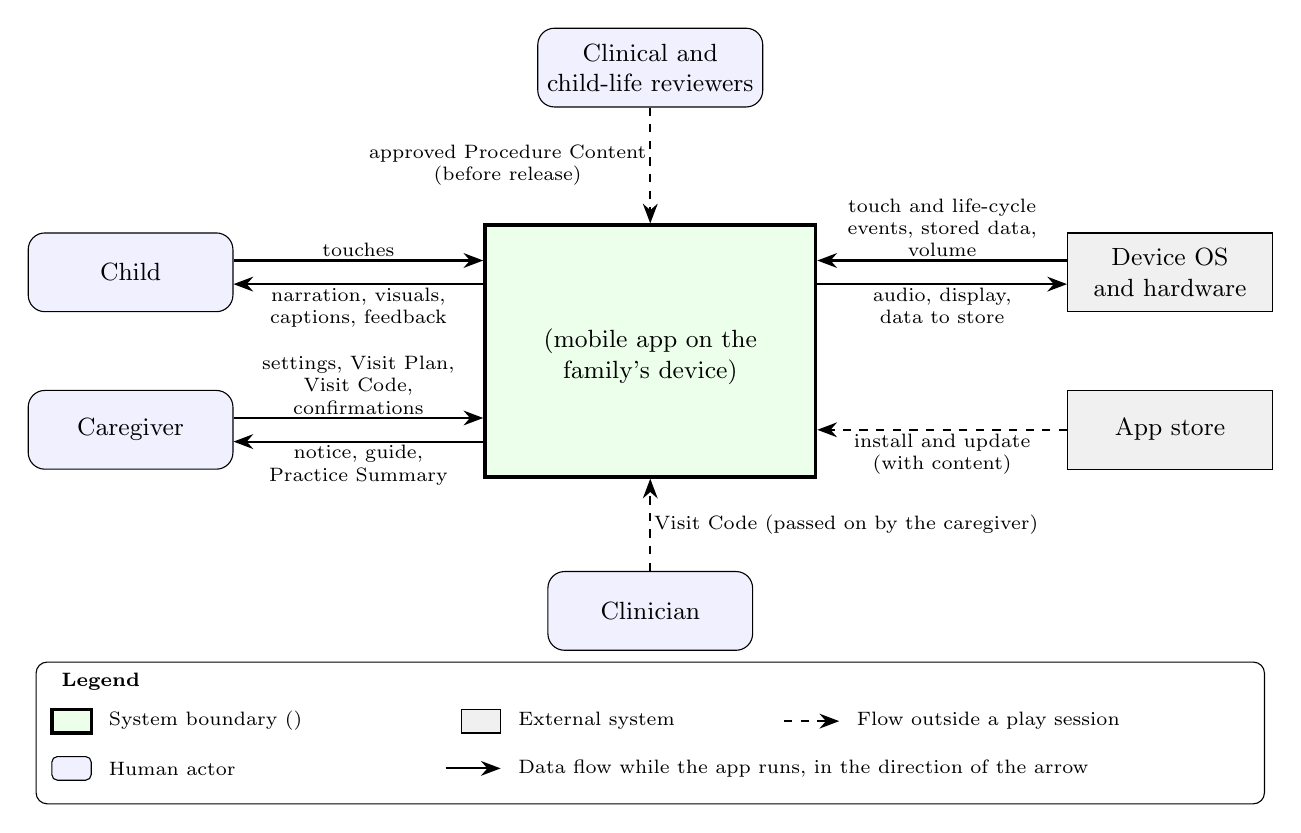
\begin{tikzpicture}[
  font=\small,
  actor/.style={draw, rounded corners=6pt, align=center, minimum width=2.6cm,
    minimum height=1.0cm, fill=blue!6},
  ext/.style={draw, align=center, minimum width=2.6cm, minimum height=1.0cm,
    fill=gray!12},
  sys/.style={draw, very thick, align=center, minimum width=4.2cm,
    minimum height=3.2cm, fill=green!8},
  flow/.style={-{Stealth[length=2.5mm]}, thick},
  offline/.style={-{Stealth[length=2.5mm]}, thick, dashed},
  lbl/.style={font=\scriptsize, align=center, fill=white, inner sep=1pt}
]
% Nodes are placed on an explicit grid (units: cm)
\node[sys] (sys) at (0, 0) {\textbf{\progname{}}\\(mobile app on the\\family's
  device)};
\node[actor] (child) at (-6.6, 1.0) {Child};
\node[actor] (care) at (-6.6, -1.0) {Caregiver};
\node[ext] (os) at (6.6, 1.0) {Device OS\\and hardware};
\node[ext] (store) at (6.6, -1.0) {App store};
\node[actor] (rev) at (0, 3.6) {Clinical and\\child-life reviewers};
\node[actor] (clin) at (0, -3.3) {Clinician};

% Child <-> system
\draw[flow] (child.east |- 0, 1.15) -- node[lbl, above] {touches}
  (sys.west |- 0, 1.15);
\draw[flow] (sys.west |- 0, 0.85) -- node[lbl, below]
  {narration, visuals,\\captions, feedback} (child.east |- 0, 0.85);
% Caregiver <-> system
\draw[flow] (care.east |- 0, -0.85) -- node[lbl, above]
  {settings, Visit Plan,\\Visit Code,\\confirmations} (sys.west |- 0, -0.85);
\draw[flow] (sys.west |- 0, -1.15) -- node[lbl, below]
  {notice, guide,\\Practice Summary} (care.east |- 0, -1.15);
% OS <-> system
\draw[flow] (os.west |- 0, 1.15) -- node[lbl, above]
  {touch and life-cycle\\events, stored data,\\volume} (sys.east |- 0, 1.15);
\draw[flow] (sys.east |- 0, 0.85) -- node[lbl, below]
  {audio, display,\\data to store} (os.west |- 0, 0.85);
% Store -> system (outside a play session)
\draw[offline] (store.west) -- node[lbl, below]
  {install and update\\(with content)} (sys.east |- store.west);
% Reviewers and clinician (outside a play session)
\draw[offline] (rev.south) -- node[lbl, left]
  {approved Procedure Content\\(before release)} (sys.north);
\draw[offline] (clin.north) -- node[lbl, right]
  {Visit Code (passed on by the caregiver)} (sys.south);

% Legend
\begin{scope}[shift={(-7.6, -4.4)}, font=\scriptsize]
  \draw[rounded corners] (-0.2, 0.45) rectangle (15.4, -1.35);
  \node[anchor=west] at (0, 0.2) {\textbf{Legend}};
  \draw[very thick, fill=green!8] (0, -0.15) rectangle (0.5, -0.45);
  \node[anchor=west] at (0.6, -0.3) {System boundary (\progname{})};
  \draw[rounded corners=2pt, fill=blue!6] (0, -0.75) rectangle (0.5, -1.05);
  \node[anchor=west] at (0.6, -0.9) {Human actor};
  \draw[fill=gray!12] (5.2, -0.15) rectangle (5.7, -0.45);
  \node[anchor=west] at (5.8, -0.3) {External system};
  \draw[flow] (5.0, -0.9) -- (5.7, -0.9);
  \node[anchor=west] at (5.8, -0.9) {Data flow while the app runs, in the
    direction of the arrow};
  \draw[offline] (9.3, -0.3) -- (10.0, -0.3);
  \node[anchor=west] at (10.1, -0.3) {Flow outside a play session};
\end{scope}
\end{tikzpicture}
\caption{System context of \progname{}}
\label{Fig_SystemContext}
\end{figure}

The responsibilities of each entity, in terms of inputs and outputs, are:

\begin{itemize}
\item \textbf{Child:} provides touch input in response to prompts.
\item \textbf{Caregiver:} installs \progname{}; acknowledges the
  Not-Medical-Advice Notice; enters settings, the Visit Plan or a Visit Code;
  supervises children younger than five; and confirms destructive actions
  such as resetting progress.
\item \textbf{Clinician:} optionally gives the family a Visit Code or tells
  them which procedures to expect; may view the Practice Summary on the
  family's device.
\item \textbf{Clinical and child-life reviewers:} approve the Procedure
  Content before it is released (\nfrref{NFR_ContentApproval},
  \nfrref{NFR_ChildLifeReview}).
\item \textbf{Device OS and hardware:} deliver touch and life-cycle events and
  the media volume level; store and return data; play audio and display
  images.
\item \textbf{App store:} delivers the installation package, including all
  Procedure Content, and updates.
\item \textbf{\progname{}:}
  \begin{itemize}
  \item present the walkthroughs and activities according to
    Section~\ref{sec_FR};
  \item validate every caregiver entry, such as a Visit Code, and reject
    invalid entries without changing existing data
    (\rref{FR_VisitCodeInvalid});
  \item check stored data for validity on launch and recover from invalid
    data (\rref{FR_CorruptProgress});
  \item protect the Caregiver Area from children (\rref{FR_CaregiverCheck});
  \item never transmit data off the device (\nfrref{NFR_NoTransmission}).
  \end{itemize}
\end{itemize}

\paragraph{Inputs and outputs.} Table~\ref{tab:InputsOutputs} lists every input
to and output from \progname{}, as requested in peer review
(\eref{E_PeerReview}). The data types are defined in
Section~\ref{sec_DataDictionary}.

\begin{longtable}{L{0.07\textwidth} L{0.25\textwidth} L{0.18\textwidth}
  L{0.39\textwidth}}
\caption{System inputs and outputs} \label{tab:InputsOutputs}\\
\toprule
\textbf{ID} & \textbf{Name} & \textbf{Source or destination} &
\textbf{Content and range}\\
\midrule
\endfirsthead
\toprule
\textbf{ID} & \textbf{Name} & \textbf{Source or destination} &
\textbf{Content and range}\\
\midrule
\endhead
\multicolumn{4}{l}{\textit{Inputs}}\\
I1 & Touch events & Child or caregiver, via OS & Touch start and end, with a
screen position; several touches may be active at once.\\
I2 & Caregiver entries & Caregiver & Notice acknowledgement, Caregiver Check
answer, settings values, Visit Plan selections, reset confirmation.\\
I3 & Visit Code & Caregiver (from clinic) & A character string; valid codes
follow the format in Section~\ref{sec_DataDictionary}. Any other string is
invalid.\\
I4 & Life-cycle events & OS & Suspend (app sent to background), resume,
terminate.\\
I5 & Media volume & OS & Device media volume, from silent to maximum.\\
I6 & Stored data & Device storage & Progress, settings, Visit Plan and notice
acknowledgement saved earlier by \progname{}; may be missing or invalid.\\
I7 & Procedure Content & Installation package & Data for each procedure, as in
Section~\ref{sec_DataEntities}.\\
\multicolumn{4}{l}{\textit{Outputs}}\\
O1 & Visual presentation & Display & Illustrations, animations, captions,
progress indicators, interaction cues, feedback.\\
O2 & Audio & Speaker or headphones & Narration and sound effects.\\
O3 & Stored data & Device storage & Progress, settings, Visit Plan and notice
acknowledgement.\\
O4 & Caregiver information & Display & Notice, procedure guide, Practice
Summary, error and confirmation messages.\\
\bottomrule
\end{longtable}

\paragraph{Functional areas.} To allow part of the requirements to be reviewed
from a subset of the inputs to a subset of the outputs,
Table~\ref{tab:FunctionalAreas} divides \progname{} into functional areas.
They describe the behaviour visible at the boundary, not a design
decomposition.

\begin{longtable}{L{0.22\textwidth} L{0.14\textwidth} L{0.14\textwidth}
  L{0.39\textwidth}}
\caption{Functional areas of \progname{}} \label{tab:FunctionalAreas}\\
\toprule
\textbf{Area} & \textbf{Inputs} & \textbf{Outputs} &
\textbf{Requirements}\\
\midrule
\endfirsthead
\toprule
\textbf{Area} & \textbf{Inputs} & \textbf{Outputs} &
\textbf{Requirements}\\
\midrule
\endhead
Procedure library & I1, I6, I7 & O1, O2 & Section~\ref{sec_FRLibrary}\\
Walkthrough player & I1, I4, I5, I7 & O1, O2 &
Sections~\ref{sec_FRWalkthrough}, \ref{sec_FRActivities},
\ref{sec_FRPresentation}\\
Progress and rewards & I6 & O1, O3 & Section~\ref{sec_FRProgress}\\
Caregiver Area & I1, I2, I3, I6 & O3, O4 & Sections~\ref{sec_FRCaregiver},
\ref{sec_FRVisitPlan}\\
Event handling & I4, I6 & O3, O4 & Section~\ref{sec_UndesiredEvents}\\
\bottomrule
\end{longtable}

\paragraph{Context of use.} \progname{} is used for health education and
preparation at home and in clinic waiting rooms. It is not mission-critical
and not safety-critical in the sense of controlling equipment or informing
clinical decisions. However, its users are young children in a medical
context, so content errors, frightening material, privacy failures and
designs that frustrate the child can cause psychological harm and reduce
cooperation. These hazards are analysed in the \hadoc{}, and the resulting
requirements are marked with a ``Hazard'' line in this document.

\subsection{User Characteristics}
\label{SecUserCharacteristics}

The users differ from the intended readers of this document
(Section~\ref{sec_IntendedReader}). The characteristics below are used to set
the usability requirements (Section~\ref{sec_Usability}) and are illustrated
by the personas in Section~\ref{sec_Personas}.

\paragraph{Children (primary users).}
\begin{itemize}
\item Aged \cst{MIN_AGE} to \cst{MAX_AGE} years. Many cannot read; older ones
  read simple words. All instructions must therefore be spoken and shown with
  pictures.
\item Have developing fine motor control: they tap imprecisely, often with
  several fingers, and may tap repeatedly.
\item Have short attention spans, which grow with age.
\item May have reduced vision at the time of use: they are eye patients, some
  wear patches or glasses, and in the waiting room their pupils may be dilated,
  making the screen look blurry and bright (\eref{E_ClinicVisit}). Some have
  colour vision deficiencies.
\item May already be anxious about the appointment, and respond strongly to
  praise and to perceived failure.
\end{itemize}

\paragraph{Caregivers.}
\begin{itemize}
\item Adults with varied education, technical experience and English
  proficiency; they can operate a smartphone app store and read simple
  English instructions.
\item Often stressed or short of time, and may use \progname{} in a busy
  waiting room.
\item Have no clinical training.
\end{itemize}

\paragraph{Clinicians.}
\label{sec_UserCharacteristicsClin}
\begin{itemize}
\item Eye-care professionals with deep clinical knowledge, who use specialized
  equipment such as the slit lamp and Optical Coherence Tomography (OCT)
  scanners for eye photos.
\item Have very little time per patient: an interaction with \progname{} must
  take seconds, not minutes.
\end{itemize}

\subsection{System Constraints}
\label{sec_Constraints}

System constraints are design decisions imposed from outside the
requirements. Each is listed with its source and rationale.

\begin{itemize}[leftmargin=1.2cm, labelwidth=1.0cm, align=left]
\item[\cdef{C_Platforms}] \progname{} shall run on consumer smartphones and
  tablets with the iOS and Android operating systems.
  \attr{Rationale}{The supervisor's project description specifies a mobile
  app (\eref{E_ProjectDescription}), and the families who will use it own
  phones and tablets with these two operating systems.}
\item[\cdef{C_Distribution}] \progname{} shall be distributed through the
  Apple App Store and Google Play.
  \attr{Rationale}{These are the channels families use to install apps; the
  stores' policies for children's apps therefore apply
  (\nfrref{NFR_StorePolicy}).}
\item[\cdef{C_Engine}] \progname{} shall be built with the Unity engine and the
  C\# language.
  \attr{Rationale}{Decided in the \dpdoc{}: Unity builds for both platforms
  from one code base, which suits a five-person team, and supports the AR
  stretch goal (\lcref{LC_AR}).}
\item[\cdef{C_Language}] The child-facing text and narration shall be in
  Canadian English.
  \attr{Rationale}{The pilot clinic is in Ontario and the team can produce and
  review content only in English. French is a likely change
  (\lcref{LC_Language}).}
\item[\cdef{C_NoServer}] \progname{} shall not depend on any server operated by
  the project.
  \attr{Rationale}{The project has no budget or staff to operate a service
  after the course ends, and the teaching assistant advised that personal
  information should remain in the clinic's existing secure systems
  (\eref{E_TAMeeting}). See \ratref{R_NoPersonalData}.}
\item[\cdef{C_Licences}] All third-party assets and libraries shall have
  licences that permit redistribution in a free app, and their notices shall be
  included with \progname{}.
  \attr{Rationale}{The project is released under the MIT licence
  (\dpdoc{}) and relies on free assets because the team has no art budget.}
\item[\cdef{C_Ethics}] Testing with children shall take place only under
  Research Ethics Board (REB) approval and with caregiver consent.
  \attr{Rationale}{Research involving children requires ethics approval; the
  clinic is confirming whether its REB must review the study
  (\eref{E_ClinicVisit}). This constrains how the usability fit criteria in
  Section~\ref{sec_Usability} can be verified.}
\end{itemize}

\subsection{Assumptions}
\label{sec_Assumptions}

This subsection was added to the template. Each assumption limits the scope
of the requirements; the requirements that depend on it are named.

\begin{itemize}[leftmargin=1.2cm, labelwidth=1.0cm, align=left]
\item[\asdef{A_CaregiverPresent}] A caregiver installs \progname{}, completes
  the first-launch steps and is nearby when a child younger than five plays.
  \attr{Affects}{\rref{FR_Notice}, \rref{FR_CaregiverCheck}.}
\item[\asdef{A_PerceiveOutput}] The child can perceive at least one of the
  narration or the visual presentation. \progname{} does not serve children who
  can perceive neither.
  \attr{Affects}{\rref{FR_Narration}, \rref{FR_MutedCaptions}.}
\item[\asdef{A_TouchScreen}] The device has a working touch screen. Audio output
  may be absent or muted.
  \attr{Affects}{Section~\ref{sec_FRActivities}.}
\item[\asdef{A_TypicalClinic}] Clinics perform each procedure broadly as
  described in its approved content. Details vary between clinics, so content
  describes the common experience and says that the child's doctor may do
  things a little differently.
  \attr{Affects}{\nfrref{NFR_ContentApproval}.}
\item[\asdef{A_KnownProcedures}] The caregiver or clinic knows which procedures
  the visit will include. When nobody does, the Visit Plan is empty and every
  procedure is offered equally.
  \attr{Affects}{\rref{FR_VisitHighlight}, \rref{FR_VisitPlanManual}.}
\item[\asdef{A_InstallBeforeVisit}] The family installs \progname{} where an
  internet connection is available, before the visit or while waiting.
  \attr{Affects}{\nfrref{NFR_Offline}, \nfrref{NFR_InstallSize}.}
\item[\asdef{A_NoTampering}] Users do not deliberately modify the stored data or
  the installed package. Accidental corruption is still handled
  (\rref{FR_CorruptProgress}).
  \attr{Affects}{\rref{FR_CorruptProgress}, \nfrref{NFR_ReleaseIntegrity}.}
\end{itemize}

% ==============================================================
\section{Stakeholder Requirements}
\label{sec_StakeholderReqs}

The stakeholder requirements state, in the stakeholders' own terms and
without reference to technology, what \progname{} must achieve. Each is traced
to the elicitation sources in Appendix~\ref{sec_AppendixA}
(Table~\ref{tab:Elicitation}) and to the use cases and requirements that
refine it.

\begin{itemize}[leftmargin=1.4cm, labelwidth=1.2cm, align=left]

\item[\srdef{SR_Familiarize}] Children shall be able to learn what happens
  during each common paediatric eye-clinic procedure before their
  appointment.
  \attr{Source}{\eref{E_ProjectDescription}, \eref{E_ClinicVisit}.}
  \attr{Refined by}{\ucref{UC_ChooseProcedure}, \ucref{UC_Walkthrough},
  \ucref{UC_KnowledgeCheck}, \ucref{UC_ReadGuide}; \rref{FR_Library},
  \rref{FR_StartProcedure}, \rref{FR_StepOrder}, \rref{FR_StoryStep},
  \rref{FR_TapTarget}, \rref{FR_KnowledgeCheck}, \rref{FR_Demonstration},
  \rref{FR_ProcedureGuide}.}

\item[\srdef{SR_ReduceAnxiety}] The preparation shall calm children rather
  than add to their worry.
  \attr{Source}{\eref{E_ProjectDescription}, \eref{E_ClinicVisit},
  \eref{E_Literature}.}
  \attr{Refined by}{\ucref{UC_Walkthrough}, \ucref{UC_KnowledgeCheck},
  \ucref{UC_HoldStill}, \ucref{UC_Interrupted}; \rref{FR_ExitWalkthrough},
  \rref{FR_SensationWarning}, \rref{FR_QuizAssist}, \rref{FR_HoldInterrupt},
  \rref{FR_HoldAssist}, \rref{FR_NoFailure}, \rref{FR_PositiveFeedback},
  \rref{FR_CaregiverSkip}, \rref{FR_Suspend}, \rref{FR_MissingContent};
  \nfrref{NFR_ChildLifeReview}, \nfrref{NFR_ContentValidation},
  \nfrref{NFR_Loudness}, \nfrref{NFR_CrashFree}.}

\item[\srdef{SR_PractiseBehaviour}] Children shall be able to practise the
  behaviours that clinicians need from them: keeping the eyes open for drops,
  keeping the head still, keeping one eye covered and following a target.
  \attr{Source}{\eref{E_ClinicVisit}.}
  \attr{Refined by}{\ucref{UC_Walkthrough}, \ucref{UC_HoldStill};
  \rref{FR_TapTarget}, \rref{FR_HoldStill}, \rref{FR_HoldInterrupt},
  \rref{FR_RepeatTap}.}

\item[\srdef{SR_AgeAppropriate}] The product shall be usable and engaging for
  children aged \cst{MIN_AGE} to \cst{MAX_AGE}, including children who cannot
  read.
  \attr{Source}{\eref{E_ProjectDescription}, \eref{E_SupervisorMeeting}.}
  \attr{Refined by}{\ucref{UC_ChooseProcedure}, \ucref{UC_Walkthrough},
  \ucref{UC_KnowledgeCheck}, \ucref{UC_HoldStill}; \rref{FR_Library},
  \rref{FR_Availability}, \rref{FR_ComingSoon}, \rref{FR_Narration},
  \rref{FR_ReplayNarration}, \rref{FR_IdlePrompt}, \rref{FR_StepProgress},
  \rref{FR_QuizAssist}, \rref{FR_HoldAssist}, \rref{FR_NoFailure},
  \rref{FR_CaregiverSkip}, \rref{FR_Captions}, \rref{FR_MutedCaptions},
  \rref{FR_VisualCue}, \rref{FR_MultiTouch}, \rref{FR_RapidTaps};
  \nfrref{NFR_IndependentUse}, \nfrref{NFR_PreReader},
  \nfrref{NFR_WalkthroughLength}, \nfrref{NFR_ChildEnjoyment},
  \nfrref{NFR_PlainLanguage}, \nfrref{NFR_TouchTarget},
  \nfrref{NFR_Inclusive}, \nfrref{NFR_ResponseTime}, \nfrref{NFR_FrameRate},
  \nfrref{NFR_LaunchTime}.}

\item[\srdef{SR_HomeAndWaitingRoom}] Families shall be able to prepare on their
  own at home and while waiting at the clinic.
  \attr{Source}{\eref{E_ProjectDescription}, \eref{E_ClinicVisit}.}
  \attr{Refined by}{\ucref{UC_FirstLaunch}, \ucref{UC_Settings},
  \ucref{UC_ResetProgress}, \ucref{UC_ReadGuide}; \rref{FR_ProcedureGuide},
  \rref{FR_Settings}, \rref{FR_Captions}, \rref{FR_MutedCaptions};
  \nfrref{NFR_IndependentUse}, \nfrref{NFR_CaregiverSUS},
  \nfrref{NFR_CaregiverSetup}, \nfrref{NFR_Offline},
  \nfrref{NFR_InstallStores}, \nfrref{NFR_InstallSize},
  \nfrref{NFR_NoAccount}.}

\item[\srdef{SR_ClinicalAccuracy}] What children are shown shall match what
  actually happens in the clinic, as confirmed by clinicians.
  \attr{Source}{\eref{E_ClinicVisit}, \eref{E_DevPlanRisks}.}
  \attr{Refined by}{\rref{FR_StepOrder}; \nfrref{NFR_ContentApproval}.}

\item[\srdef{SR_Honesty}] Children shall be told truthfully about unpleasant
  sensations, such as drops that burn or bright lights.
  \attr{Source}{\eref{E_ClinicVisit}, \eref{E_DevPlanRisks}.}
  \attr{Refined by}{\ucref{UC_Walkthrough}; \rref{FR_SensationWarning},
  \rref{FR_RapidTaps}; \nfrref{NFR_ContentApproval},
  \nfrref{NFR_ChildLifeReview}.}

\item[\srdef{SR_Rewards}] Children shall be rewarded for practising, to
  motivate them to finish.
  \attr{Source}{\eref{E_ProjectDescription}.}
  \attr{Refined by}{\ucref{UC_Walkthrough}, \ucref{UC_ViewStickers},
  \ucref{UC_ResetProgress}, \ucref{UC_Interrupted}; \rref{FR_Availability},
  \rref{FR_Completion}, \rref{FR_AwardSticker}, \rref{FR_StickerBook},
  \rref{FR_PersistProgress}, \rref{FR_ResetProgress}, \rref{FR_Suspend},
  \rref{FR_Terminate}, \rref{FR_CorruptProgress}, \rref{FR_SaveFailure};
  \nfrref{NFR_ChildEnjoyment}, \nfrref{NFR_ProgressDurability}.}

\item[\srdef{SR_VisitRelevant}] Preparation shall be able to focus on the
  procedures planned for the child's own visit, as chosen by the clinician or
  family.
  \attr{Source}{\eref{E_TAMeeting}, \eref{E_ProblemStatement}.}
  \attr{Refined by}{\ucref{UC_ChooseProcedure}, \ucref{UC_SetVisitPlan},
  \ucref{UC_EnterVisitCode}; \rref{FR_VisitHighlight},
  \rref{FR_VisitPlanManual}, \rref{FR_VisitCode}, \rref{FR_VisitCodeInvalid};
  \nfrref{NFR_CaregiverSetup}, \nfrref{NFR_VisitCodePrivacy}.}

\item[\srdef{SR_NoPHI}] The children's app shall not hold personal health
  information; such information shall stay in the clinic's existing secure
  systems.
  \attr{Source}{\eref{E_TAMeeting}.}
  \attr{Refined by}{\ucref{UC_FirstLaunch}, \ucref{UC_EnterVisitCode};
  \rref{FR_VisitCode}; \nfrref{NFR_NoAccount}, \nfrref{NFR_Uninstall},
  \nfrref{NFR_NoPersonalInfo}, \nfrref{NFR_NoTransmission},
  \nfrref{NFR_VisitCodePrivacy}, \nfrref{NFR_PrivacyLaw}.}

\item[\srdef{SR_NotMedicalAdvice}] Families shall understand that the product
  is a preparation aid and not medical advice.
  \attr{Source}{\eref{E_InstructorHA}.}
  \attr{Refined by}{\ucref{UC_FirstLaunch}, \ucref{UC_ReadGuide};
  \rref{FR_Notice}, \rref{FR_NoticeAccess}; \nfrref{NFR_NotMedicalDevice}.}

\item[\srdef{SR_ShowPractice}] Caregivers, clinicians and the evaluation study
  shall be able to see which preparation activities a child has completed.
  \attr{Source}{\eref{E_ProjectDescription}, \eref{E_ProblemStatement}.}
  \attr{Refined by}{\ucref{UC_ShowSummary}; \rref{FR_Completion},
  \rref{FR_PersistProgress}, \rref{FR_PracticeSummary};
  \nfrref{NFR_ProgressDurability}.}

\item[\srdef{SR_MobileDevices}] The product shall work on the phones and tablets
  that families already own.
  \attr{Source}{\eref{E_ProjectDescription}, \eref{E_ProblemStatement}.}
  \attr{Refined by}{\nfrref{NFR_Platforms}, \nfrref{NFR_ScreenSizes},
  \nfrref{NFR_FrameRate}, \nfrref{NFR_LaunchTime}, \nfrref{NFR_CrashFree},
  \nfrref{NFR_InstallStores}, \nfrref{NFR_InstallSize},
  \nfrref{NFR_StorePolicy}.}

\item[\srdef{SR_Offline}] The product shall work where there is no internet
  connection, such as in hospital waiting rooms.
  \attr{Source}{\eref{E_DevPlanRisks}.}
  \attr{Refined by}{\nfrref{NFR_Offline}, \nfrref{NFR_NoTransmission}.}

\item[\srdef{SR_LowVision}] Children with reduced vision, including dilated
  pupils, patches or colour vision deficiency, shall be able to use the
  product.
  \attr{Source}{\eref{E_ClinicVisit}.}
  \attr{Refined by}{\ucref{UC_Settings}; \rref{FR_Narration},
  \rref{FR_Settings}; \nfrref{NFR_TouchTarget}, \nfrref{NFR_Contrast},
  \nfrref{NFR_NoColourOnly}, \nfrref{NFR_Accessibility}.}

\item[\srdef{SR_ChildSafe}] The product shall be safe and appropriate for young
  children: free of advertising, purchases, frightening content and designs
  that encourage compulsive use, and compliant with the rules for children's
  apps.
  \attr{Source}{\eref{E_InstructorHA}, \eref{E_ProblemStatement}.}
  \attr{Refined by}{\rref{FR_CaregiverCheck}; \nfrref{NFR_ChildLifeReview},
  \nfrref{NFR_Flashing}, \nfrref{NFR_Loudness}, \nfrref{NFR_Inclusive},
  \nfrref{NFR_NoPersonalInfo}, \nfrref{NFR_NoTransmission},
  \nfrref{NFR_ReleaseIntegrity}, \nfrref{NFR_NoCompulsiveDesign},
  \nfrref{NFR_NoAdsPurchases}, \nfrref{NFR_StorePolicy}.}

\item[\srdef{SR_MoreProcedures}] Further clinic procedures shall be addable
  over time.
  \attr{Source}{\eref{E_ClinicVisit}.}
  \attr{Refined by}{\nfrref{NFR_AddProcedure}, \nfrref{NFR_ContentValidation},
  \nfrref{NFR_LikelyChangeEffort}, \nfrref{NFR_Understandability}.}

\end{itemize}

% ==============================================================
\section{User Personas}
\label{sec_Personas}

The personas below are fictional. They combine the user characteristics in
Section~\ref{SecUserCharacteristics} with what the team observed at the clinic
(\eref{E_ClinicVisit}) and learned from the supervisor
(\eref{E_ProjectDescription}). They will be checked against the interviews and
usability sessions recorded in the project's Client Interview Report and
Usability Report.

\subsection{Persona 1: Maya, a four-year-old first-time patient}
\begin{itemize}
\item Name: Maya, aged 4.
\item Description: Referred after a school vision screening. Cannot read yet;
  knows numbers to ten. Loves stickers and animal pictures. Cried at her last
  vaccination and has asked whether the eye doctor will give her a needle.
\item Goals: Know what the doctor will do; know that nothing will hurt for
  long; have something to show her grandmother afterwards.
\item Frustrations: Long instructions; things she cannot do on the first try;
  being told she got something ``wrong''.
\item Technical Ability: Uses a tablet daily for videos and simple games by
  tapping; taps quickly and often with several fingers; cannot type or read
  menus.
\end{itemize}

\subsection{Persona 2: Theo, a seven-year-old before eye-muscle surgery}
\begin{itemize}
\item Name: Theo, aged 7.
\item Description: Has a turned eye and wears a patch for two hours a day.
  Needs careful alignment measurements before surgery. Has had several visits
  and hates the drops, which burned last time. Reads short words.
\item Goals: Understand why he needs the tests; feel in control; finish every
  activity and collect all the stickers.
\item Frustrations: Babyish content; long waits; surprises.
\item Technical Ability: Plays phone games confidently; can navigate menus with
  pictures; uses the device with one eye patched.
\end{itemize}

\subsection{Persona 3: Amira, a parent preparing two children}
\begin{itemize}
\item Name: Amira, aged 36.
\item Description: Works shifts and has two children; English is her second
  language. The clinic letter told her the visit takes up to three hours and
  includes ``dilation''. She will use \progname{} the night before and in the
  waiting room.
\item Goals: Explain the visit to her child in a way the child understands;
  know which tests to practise; know what she can do to help.
\item Frustrations: Sign-ups and accounts; apps that ask for personal
  information; medical words; ads in children's apps.
\item Technical Ability: Uses messaging, banking and app-store apps daily;
  prefers short instructions with pictures.
\end{itemize}

\subsection{Persona 4: Dr.~Okafor, a paediatric orthoptist}
\begin{itemize}
\item Name: Dr.~Okafor, aged 48.
\item Description: Performs vision and alignment testing in a busy clinic, with
  about 15 minutes per patient. Has seen many examinations abandoned because a
  child would not keep still.
\item Goals: Patients who arrive knowing what to do; a quick way to tell a
  family which tests to practise; confidence that the app shows the procedures
  correctly.
\item Frustrations: Anything that adds steps to the clinic workflow; content
  that promises a test will not be uncomfortable.
\item Technical Ability: Uses the clinic's record system and equipment
  software daily; has no time to learn a new tool.
\end{itemize}

% ==============================================================
\section{Use Cases}
\label{sec_UseCases}

The use cases describe how the actors in Figure~\ref{Fig_SystemContext}
interact with \progname{} to reach their goals. Each use case names the
stakeholder requirements it traces to; the functional requirements that
implement each use case are listed in Table~\ref{tab:SR2UC2FRtm}.

\refstepcounter{ucnum} \label{UC_FirstLaunch}
\subsection{\ucref{UC_FirstLaunch}: Launch \progname{} for the First Time}

\textbf{Primary Actor:} Caregiver.\quad \textbf{Traces:}
\srref{SR_NotMedicalAdvice}, \srref{SR_HomeAndWaitingRoom},
\srref{SR_NoPHI}.

\textbf{Preconditions}
\begin{itemize}
\item \progname{} has been installed and has never been opened, or its data
  has been cleared.
\end{itemize}

\textbf{Main Success Scenario}
\begin{enumerate}
\item The caregiver opens \progname{}.
\item \progname{} shows and reads the Not-Medical-Advice Notice.
\item The caregiver acknowledges the notice.
\item \progname{} shows the Procedure Library, ready for the child.
\end{enumerate}

\textbf{Alternative Flows}
\begin{itemize}
\item 3a. The caregiver closes \progname{} without acknowledging: the notice is
  shown again at the next launch.
\end{itemize}

\textbf{Postconditions}
\begin{itemize}
\item The acknowledgement is stored; no personal information has been
  requested.
\end{itemize}

\refstepcounter{ucnum} \label{UC_ChooseProcedure}
\subsection{\ucref{UC_ChooseProcedure}: Choose a Procedure to Practise}

\textbf{Primary Actor:} Child.\quad \textbf{Traces:}
\srref{SR_Familiarize}, \srref{SR_AgeAppropriate},
\srref{SR_VisitRelevant}.

\textbf{Preconditions}
\begin{itemize}
\item The notice has been acknowledged and the Procedure Library is shown.
\end{itemize}

\textbf{Main Success Scenario}
\begin{enumerate}
\item \progname{} shows a picture card for every procedure, with its
  availability, and lists Visit Plan procedures first.
\item The child taps a card; \progname{} speaks the procedure's name.
\item \progname{} starts the walkthrough (\ucref{UC_Walkthrough}).
\end{enumerate}

\textbf{Alternative Flows}
\begin{itemize}
\item 2a. The card is Coming Soon: \progname{} says that this visit is not
  ready yet and stays in the library.
\end{itemize}

\textbf{Postconditions}
\begin{itemize}
\item The chosen walkthrough is at its first step.
\end{itemize}

\refstepcounter{ucnum} \label{UC_Walkthrough}
\subsection{\ucref{UC_Walkthrough}: Complete a Procedure Walkthrough}

\textbf{Primary Actor:} Child (a caregiver may watch).\quad
\textbf{Traces:} \srref{SR_Familiarize}, \srref{SR_ReduceAnxiety},
\srref{SR_Honesty}, \srref{SR_PractiseBehaviour}, \srref{SR_Rewards},
\srref{SR_AgeAppropriate}.

\textbf{Preconditions}
\begin{itemize}
\item A walkthrough has been started.
\end{itemize}

\textbf{Main Success Scenario}
\begin{enumerate}
\item \progname{} presents the current step: the doctor character speaks the
  narration, the caption is shown, and an illustration shows the clinic.
\item If the step involves a sensation, the doctor first says what it will
  feel like and that it passes.
\item The child completes the step's activity (for example
  \ucref{UC_KnowledgeCheck} or \ucref{UC_HoldStill}).
\item \progname{} praises the child and moves to the next step.
\item Steps 1 to 4 repeat until the last step is completed.
\item \progname{} celebrates and awards the procedure's sticker
  (\ucref{UC_ViewStickers}).
\end{enumerate}

\textbf{Alternative Flows}
\begin{itemize}
\item 3a. The child does nothing for a while: \progname{} repeats the prompt
  and shows where to tap.
\item 3b. The child wants to hear the narration again: the child taps the
  replay control.
\item 3c. The child leaves the walkthrough: \progname{} returns to the library
  and progress is unchanged.
\item 3d. The app is interrupted: see \ucref{UC_Interrupted}.
\end{itemize}

\textbf{Postconditions}
\begin{itemize}
\item The procedure is recorded as completed with today's date, and its
  sticker is in the Sticker Book.
\end{itemize}

\refstepcounter{ucnum} \label{UC_KnowledgeCheck}
\subsection{\ucref{UC_KnowledgeCheck}: Answer a Knowledge Check}

\textbf{Primary Actor:} Child.\quad \textbf{Traces:}
\srref{SR_Familiarize}, \srref{SR_ReduceAnxiety},
\srref{SR_AgeAppropriate}.

\textbf{Preconditions}
\begin{itemize}
\item The current step is a Knowledge Check.
\end{itemize}

\textbf{Main Success Scenario}
\begin{enumerate}
\item \progname{} asks a question aloud and shows two or three picture
  answers.
\item The child taps the correct picture.
\item \progname{} confirms and explains the answer; the step is complete.
\end{enumerate}

\textbf{Alternative Flows}
\begin{itemize}
\item 2a. The child taps a wrong picture: \progname{} gives an encouraging hint
  and the question stays open.
\item 2b. The child has answered wrongly \cst{QUIZ_ASSIST_THRESHOLD} times:
  \progname{} highlights the correct picture.
\end{itemize}

\textbf{Postconditions}
\begin{itemize}
\item The child has heard the correct answer explained.
\end{itemize}

\refstepcounter{ucnum} \label{UC_HoldStill}
\subsection{\ucref{UC_HoldStill}: Practise Keeping Still}

\textbf{Primary Actor:} Child.\quad \textbf{Traces:}
\srref{SR_PractiseBehaviour}, \srref{SR_ReduceAnxiety},
\srref{SR_AgeAppropriate}.

\textbf{Preconditions}
\begin{itemize}
\item The current step is a Hold Still activity, such as keeping the eyes open
  for the drops or keeping the head on the slit lamp rest.
\end{itemize}

\textbf{Main Success Scenario}
\begin{enumerate}
\item \progname{} explains what to keep still and asks the child to press and
  hold the hold control.
\item The child presses and holds; a progress indicator fills.
\item After the required time, \progname{} shows the outcome (for example, the
  drop going in) and praises the child.
\end{enumerate}

\textbf{Alternative Flows}
\begin{itemize}
\item 2a. The child lets go early: \progname{} explains, kindly, that this is
  like blinking and the doctor will simply try again; the indicator resets and
  the child can press again.
\item 2b. The child has let go early \cst{HOLD_ASSIST_THRESHOLD} times: the
  required time becomes \cst{HOLD_DURATION_ASSISTED}.
\end{itemize}

\textbf{Postconditions}
\begin{itemize}
\item The step is complete.
\end{itemize}

\refstepcounter{ucnum} \label{UC_ViewStickers}
\subsection{\ucref{UC_ViewStickers}: Earn and View Stickers}

\textbf{Primary Actor:} Child.\quad \textbf{Traces:} \srref{SR_Rewards}.

\textbf{Preconditions}
\begin{itemize}
\item The library is shown, or a walkthrough has just been completed.
\end{itemize}

\textbf{Main Success Scenario}
\begin{enumerate}
\item The child opens the Sticker Book.
\item \progname{} shows each earned sticker and an empty outline for each
  sticker not yet earned.
\end{enumerate}

\textbf{Alternative Flows}
\begin{itemize}
\item 1a. The child has just completed a procedure for the first time: the new
  sticker is added with a celebration before the book is shown.
\item 1b. The child repeats a completed procedure: the celebration plays again
  but no duplicate sticker is added.
\end{itemize}

\textbf{Postconditions}
\begin{itemize}
\item Stickers are unchanged by viewing.
\end{itemize}

\refstepcounter{ucnum} \label{UC_SetVisitPlan}
\subsection{\ucref{UC_SetVisitPlan}: Choose the Procedures for the Next Visit}

\textbf{Primary Actor:} Caregiver.\quad \textbf{Traces:}
\srref{SR_VisitRelevant}.

\textbf{Preconditions}
\begin{itemize}
\item The caregiver knows, from the clinic letter or clinician, which
  procedures to expect.
\end{itemize}

\textbf{Main Success Scenario}
\begin{enumerate}
\item The caregiver passes the Caregiver Check and opens the Visit Plan.
\item \progname{} lists every procedure with a description.
\item The caregiver selects the expected procedures and saves.
\item The library now marks and lists those procedures first.
\end{enumerate}

\textbf{Alternative Flows}
\begin{itemize}
\item 3a. The caregiver clears the plan: all procedures are listed equally.
\end{itemize}

\textbf{Postconditions}
\begin{itemize}
\item The Visit Plan is stored.
\end{itemize}

\refstepcounter{ucnum} \label{UC_EnterVisitCode}
\subsection{\ucref{UC_EnterVisitCode}: Enter a Visit Code from the Clinic}

\textbf{Primary Actor:} Caregiver (secondary: clinician).\quad
\textbf{Traces:} \srref{SR_VisitRelevant}, \srref{SR_NoPHI}.

\textbf{Preconditions}
\begin{itemize}
\item The clinic has given the family a Visit Code, for example printed on the
  appointment letter.
\end{itemize}

\textbf{Main Success Scenario}
\begin{enumerate}
\item The caregiver passes the Caregiver Check and chooses to enter a code.
\item The caregiver enters the code.
\item \progname{} validates the code, shows the procedures it lists and asks
  for confirmation.
\item The caregiver confirms; the Visit Plan is replaced by those procedures.
\end{enumerate}

\textbf{Alternative Flows}
\begin{itemize}
\item 3a. The code is invalid: \progname{} explains that the code was not
  recognized and the existing plan is unchanged.
\item 4a. The caregiver cancels: the existing plan is unchanged.
\end{itemize}

\textbf{Postconditions}
\begin{itemize}
\item The Visit Plan matches the code; no personal information was entered or
  stored.
\end{itemize}

\refstepcounter{ucnum} \label{UC_Settings}
\subsection{\ucref{UC_Settings}: Adjust Sound and Caption Settings}

\textbf{Primary Actor:} Caregiver.\quad \textbf{Traces:}
\srref{SR_LowVision}, \srref{SR_HomeAndWaitingRoom}.

\textbf{Preconditions}
\begin{itemize}
\item The caregiver has passed the Caregiver Check.
\end{itemize}

\textbf{Main Success Scenario}
\begin{enumerate}
\item The caregiver opens Settings.
\item The caregiver changes the narration volume, turns sound effects on or
  off, or turns captions on or off.
\item \progname{} applies each change immediately and stores it.
\end{enumerate}

\textbf{Alternative Flows}
\begin{itemize}
\item None.
\end{itemize}

\textbf{Postconditions}
\begin{itemize}
\item The settings persist across launches.
\end{itemize}

\refstepcounter{ucnum} \label{UC_ResetProgress}
\subsection{\ucref{UC_ResetProgress}: Reset Progress}

\textbf{Primary Actor:} Caregiver.\quad \textbf{Traces:}
\srref{SR_Rewards}, \srref{SR_HomeAndWaitingRoom}.

\textbf{Preconditions}
\begin{itemize}
\item The caregiver has passed the Caregiver Check, for example to let a
  younger sibling start afresh.
\end{itemize}

\textbf{Main Success Scenario}
\begin{enumerate}
\item The caregiver chooses to reset progress.
\item \progname{} states what will be erased and asks for confirmation.
\item The caregiver confirms.
\item \progname{} erases all completions and stickers.
\end{enumerate}

\textbf{Alternative Flows}
\begin{itemize}
\item 3a. The caregiver cancels: nothing is erased.
\end{itemize}

\textbf{Postconditions}
\begin{itemize}
\item No procedure is completed and the Sticker Book is empty; settings, the
  Visit Plan and the notice acknowledgement are kept.
\end{itemize}

\refstepcounter{ucnum} \label{UC_Interrupted}
\subsection{\ucref{UC_Interrupted}: Recover from an Interruption}

\textbf{Primary Actor:} Device OS (on behalf of the child).\quad
\textbf{Traces:} \srref{SR_ReduceAnxiety}, \srref{SR_Rewards}.

\textbf{Preconditions}
\begin{itemize}
\item A walkthrough is in progress.
\end{itemize}

\textbf{Main Success Scenario}
\begin{enumerate}
\item A phone call or other event sends \progname{} to the background.
\item \progname{} pauses narration and animation; an active hold ends without
  counting as an interruption.
\item The child returns to \progname{}.
\item \progname{} resumes the same step.
\end{enumerate}

\textbf{Alternative Flows}
\begin{itemize}
\item 1a. The OS or the user terminates \progname{}, or the battery runs out:
  at the next launch \progname{} opens the library with all earlier progress
  intact; the interrupted walkthrough starts again from its first step.
\end{itemize}

\textbf{Postconditions}
\begin{itemize}
\item No recorded progress has been lost.
\end{itemize}

\refstepcounter{ucnum} \label{UC_ShowSummary}
\subsection{\ucref{UC_ShowSummary}: Show the Practice Summary at the Clinic}

\textbf{Primary Actor:} Caregiver (secondary: clinician).\quad
\textbf{Traces:} \srref{SR_ShowPractice}.

\textbf{Preconditions}
\begin{itemize}
\item The family is at the appointment, and the clinician asks what the child
  has practised.
\end{itemize}

\textbf{Main Success Scenario}
\begin{enumerate}
\item The caregiver passes the Caregiver Check and opens the Practice Summary.
\item \progname{} lists each procedure, whether it was completed and the date of
  the most recent completion, under a statement that this is a practice record
  and not a clinical assessment.
\item The clinician reads the summary on the caregiver's device.
\end{enumerate}

\textbf{Alternative Flows}
\begin{itemize}
\item 2a. Nothing has been completed: the summary says so.
\end{itemize}

\textbf{Postconditions}
\begin{itemize}
\item No data has left the device.
\end{itemize}

\refstepcounter{ucnum} \label{UC_ReadGuide}
\subsection{\ucref{UC_ReadGuide}: Read About a Procedure as a Caregiver}

\textbf{Primary Actor:} Caregiver.\quad \textbf{Traces:}
\srref{SR_Familiarize}, \srref{SR_HomeAndWaitingRoom},
\srref{SR_NotMedicalAdvice}.

\textbf{Preconditions}
\begin{itemize}
\item The caregiver has passed the Caregiver Check.
\end{itemize}

\textbf{Main Success Scenario}
\begin{enumerate}
\item The caregiver opens the procedure guide and selects a procedure.
\item \progname{} shows a plain-language description of what the child will
  experience and how the caregiver can help, followed by the
  Not-Medical-Advice Notice.
\end{enumerate}

\textbf{Alternative Flows}
\begin{itemize}
\item None.
\end{itemize}

\textbf{Postconditions}
\begin{itemize}
\item None; reading changes no data.
\end{itemize}

% ==============================================================
\section{Functional Requirements}
\label{sec_FR}

The functional requirements state what \progname{} shall do. They refine the
stakeholder requirements (Section~\ref{sec_StakeholderReqs}) and the use cases
(Section~\ref{sec_UseCases}). Normal operation is specified in
Sections~\ref{sec_FRLibrary} to \ref{sec_FRPresentation}, the handling of
undesired events in Section~\ref{sec_UndesiredEvents}, and the exact rules of
the activities, together with the most critical properties, in the formal
specification of Section~\ref{sec_FormalSpec}. Where an FR and
Section~\ref{sec_FormalSpec} describe the same behaviour, the formal
specification is authoritative.

\subsection{Procedure Library and Navigation}
\label{sec_FRLibrary}

\begin{itemize}[leftmargin=1.4cm, labelwidth=1.2cm, align=left]

\item[\frdef{FR_Library}] \progname{} shall show a Procedure Library containing
  one card for every procedure in the Procedure Catalogue, each with a
  picture of the procedure and a spoken name that plays when the card is
  tapped.
  \attr{Priority}{High.}
  \attr{Traces}{\srref{SR_Familiarize}, \srref{SR_AgeAppropriate};
  \ucref{UC_ChooseProcedure}.}
  \attr{Supports}{\nfrref{NFR_PreReader}, \nfrref{NFR_IndependentUse}.}

\item[\frdef{FR_Availability}] Each card shall show the procedure's
  Availability State, $\sm{avail}(p, C)$, as defined in
  Section~\ref{sec_FormalAvail}.
  \attr{Rationale}{Every procedure is available from the start, with no
  unlocking order (\ratref{R_NoLocking}).}
  \attr{Priority}{High.}
  \attr{Traces}{\srref{SR_Rewards}, \srref{SR_AgeAppropriate};
  \ucref{UC_ChooseProcedure}.}
  \attr{Supports}{\nfrref{NFR_IndependentUse}.}

\item[\frdef{FR_StartProcedure}] When the child selects a procedure whose
  Availability State is Available or Completed, \progname{} shall start its
  walkthrough at the first step.
  \attr{Priority}{High.}
  \attr{Traces}{\srref{SR_Familiarize}; \ucref{UC_ChooseProcedure},
  \ucref{UC_Walkthrough}.}
  \attr{Supports}{\nfrref{NFR_IndependentUse}.}

\item[\frdef{FR_ComingSoon}] When the child selects a Coming Soon procedure,
  \progname{} shall say that this procedure is not ready yet and shall remain
  in the library.
  \attr{Rationale}{Showing every procedure of the catalogue, even before its
  content exists, shows the child the whole visit.}
  \attr{Priority}{Low.}
  \attr{Traces}{\srref{SR_AgeAppropriate}; \ucref{UC_ChooseProcedure}.}
  \attr{Supports}{\nfrref{NFR_PreReader}.}

\item[\frdef{FR_VisitHighlight}] When the Visit Plan is not empty, the library
  shall mark the procedures in the Visit Plan and list them before all other
  procedures, in the order given in Section~\ref{sec_FormalAvail}.
  \attr{Priority}{Medium.}
  \attr{Traces}{\srref{SR_VisitRelevant}; \ucref{UC_ChooseProcedure},
  \ucref{UC_SetVisitPlan}.}
  \attr{Supports}{\nfrref{NFR_IndependentUse}.}
  \attr{Hazard}{SSR6.}

\item[\frdef{FR_ExitWalkthrough}] \progname{} shall allow the child to leave a
  walkthrough at any step and return to the library. Leaving shall not change
  the Progress.
  \attr{Rationale}{A child who becomes upset must be able to stop at once.}
  \attr{Priority}{High.}
  \attr{Traces}{\srref{SR_ReduceAnxiety}; \ucref{UC_Walkthrough}.}
  \attr{Supports}{\nfrref{NFR_ProgressDurability}.}

\end{itemize}

\subsection{Procedure Walkthroughs}
\label{sec_FRWalkthrough}

\begin{itemize}[leftmargin=1.4cm, labelwidth=1.2cm, align=left]

\item[\frdef{FR_StepOrder}] \progname{} shall present the steps of a
  walkthrough one at a time, in the order defined by the procedure's Procedure
  Content.
  \attr{Rationale}{The order of the steps mirrors the order in the clinic,
  which the clinical reviewer approves (\nfrref{NFR_ContentApproval}).}
  \attr{Priority}{High.}
  \attr{Traces}{\srref{SR_Familiarize}, \srref{SR_ClinicalAccuracy};
  \ucref{UC_Walkthrough}.}
  \attr{Supports}{\nfrref{NFR_ContentApproval}.}

\item[\frdef{FR_Narration}] For every narration line of a step, \progname{}
  shall play the line's recorded or synthesized speech and display its
  caption text while the line plays.
  \attr{Rationale}{Most children in the target range cannot read
  (Section~\ref{SecUserCharacteristics}); the caption serves caregivers,
  older children and silent devices.}
  \attr{Priority}{High.}
  \attr{Traces}{\srref{SR_AgeAppropriate}, \srref{SR_LowVision};
  \ucref{UC_Walkthrough}.}
  \attr{Supports}{\nfrref{NFR_PreReader}.}

\item[\frdef{FR_SensationWarning}] For every step that has a Sensation Tag,
  \progname{} shall present the step's sensation narration in full before the
  step's activity accepts input. The sensation narration shall not be
  skippable.
  \attr{Rationale}{Clinicians reported that the drops burn and are a major
  source of anxiety (\eref{E_ClinicVisit}). A child who is told in advance
  what a sensation feels like, and that it passes, is not surprised; a child
  who is told that nothing will hurt may lose trust (see
  \ratref{R_HonestContent}).}
  \attr{Priority}{High.}
  \attr{Traces}{\srref{SR_Honesty}, \srref{SR_ReduceAnxiety};
  \ucref{UC_Walkthrough}.}
  \attr{Supports}{\nfrref{NFR_ContentApproval}, \nfrref{NFR_ChildLifeReview}.}
  \attr{Hazard}{SSR2.}

\item[\frdef{FR_ReplayNarration}] \progname{} shall let the child replay the
  current step's narration at any time during the step.
  \attr{Priority}{Medium.}
  \attr{Traces}{\srref{SR_AgeAppropriate}; \ucref{UC_Walkthrough}.}
  \attr{Supports}{\nfrref{NFR_PreReader}.}

\item[\frdef{FR_IdlePrompt}] When an activity has waited for input for
  \cst{IDLE_PROMPT_TIME} without receiving any, \progname{} shall replay the
  activity's prompt and visually indicate the element to interact with. This
  shall repeat after each further \cst{IDLE_PROMPT_TIME} without input.
  \attr{Rationale}{Young children often stop when unsure what to do; a
  repeated, pointed prompt lets them continue without an adult.}
  \attr{Priority}{Medium.}
  \attr{Traces}{\srref{SR_AgeAppropriate}; \ucref{UC_Walkthrough}.}
  \attr{Supports}{\nfrref{NFR_IndependentUse}, \nfrref{NFR_PreReader}.}

\item[\frdef{FR_StepProgress}] During a walkthrough, \progname{} shall display
  the number of steps completed relative to the total number of steps, using a
  non-numeric indicator.
  \attr{Rationale}{Seeing the end approach keeps children motivated; the
  indicator is non-numeric because many users cannot count to the number of
  steps.}
  \attr{Priority}{Low.}
  \attr{Traces}{\srref{SR_AgeAppropriate}; \ucref{UC_Walkthrough}.}
  \attr{Supports}{\nfrref{NFR_ChildEnjoyment}.}

\item[\frdef{FR_Completion}] When the last step of a walkthrough is completed,
  \progname{} shall update the Progress as defined by $\sm{complete}$ in
  Section~\ref{sec_FormalProgress}, recording the procedure as completed on the
  current date.
  \attr{Priority}{High.}
  \attr{Traces}{\srref{SR_Rewards}, \srref{SR_ShowPractice};
  \ucref{UC_Walkthrough}.}
  \attr{Supports}{\nfrref{NFR_ProgressDurability}.}

\end{itemize}

\subsection{Practice Activities}
\label{sec_FRActivities}

Each step has exactly one of the activity types below, which are the rules of
the game. The parameters of each activity, such as its prompt and its target,
are part of the Procedure Content (Section~\ref{sec_DataDictionary}). The
precise rules are given in Section~\ref{sec_FormalSpec}.

\begin{itemize}[leftmargin=1.4cm, labelwidth=1.2cm, align=left]

\item[\frdef{FR_StoryStep}] For a \emph{Story} step, \progname{} shall complete
  the step when all of its narration lines have been presented and the child
  then taps the continue control.
  \attr{Priority}{High.}
  \attr{Traces}{\srref{SR_Familiarize}; \ucref{UC_Walkthrough}.}
  \attr{Supports}{\nfrref{NFR_IndependentUse}.}

\item[\frdef{FR_TapTarget}] For a \emph{Tap Target} step (for example, ``tap the
  chair to sit in it''), \progname{} shall complete the step when the child taps
  the step's target. Taps elsewhere shall have no effect on the step.
  \attr{Priority}{High.}
  \attr{Traces}{\srref{SR_PractiseBehaviour}, \srref{SR_Familiarize};
  \ucref{UC_Walkthrough}.}
  \attr{Supports}{\nfrref{NFR_IndependentUse}.}

\item[\frdef{FR_KnowledgeCheck}] For a \emph{Knowledge Check} step,
  \progname{} shall speak the question, show its picture answers, and evaluate
  each answer the child taps as defined in Section~\ref{sec_FormalQuiz}: a
  correct answer plays the explanation and completes the step; an incorrect
  answer plays an encouraging hint and leaves the question open.
  \attr{Priority}{High.}
  \attr{Traces}{\srref{SR_Familiarize}; \ucref{UC_KnowledgeCheck}.}
  \attr{Supports}{\nfrref{NFR_PreReader}.}

\item[\frdef{FR_QuizAssist}] After \cst{QUIZ_ASSIST_THRESHOLD} incorrect answers
  to the same question, \progname{} shall visually highlight the correct answer
  until it is chosen.
  \attr{Rationale}{The aim is that the child hears the right answer
  explained, not that the child is tested; the highlight guarantees the
  question ends after a few attempts.}
  \attr{Priority}{Medium.}
  \attr{Traces}{\srref{SR_AgeAppropriate}, \srref{SR_ReduceAnxiety};
  \ucref{UC_KnowledgeCheck}.}
  \attr{Supports}{\nfrref{NFR_IndependentUse},
  \nfrref{NFR_WalkthroughLength}.}
  \attr{Hazard}{SSR7.}

\item[\frdef{FR_HoldStill}] For a \emph{Hold Still} step, \progname{} shall
  complete the step when the child keeps contact with the hold control for the
  required duration $d(k)$ without releasing it, and shall show the fraction of
  the duration held, as defined in Section~\ref{sec_FormalHold}.
  \attr{Rationale}{Holding a finger still on the screen is a concrete stand-in
  for keeping the eyes open or the head still, which the child cannot practise
  directly on a touch screen (\ratref{R_HoldMetaphor}).}
  \attr{Priority}{High.}
  \attr{Traces}{\srref{SR_PractiseBehaviour}; \ucref{UC_HoldStill}.}
  \attr{Supports}{\nfrref{NFR_IndependentUse}.}

\item[\frdef{FR_HoldInterrupt}] When the child releases the hold control before
  the required duration has elapsed, \progname{} shall reset the held fraction
  to zero, play the step's interruption narration and accept a new attempt.
  \attr{Rationale}{The narration connects the release to the real event (a
  blink makes the drop land on the eyelid, so the doctor tries again) without
  calling it a failure.}
  \attr{Priority}{High.}
  \attr{Traces}{\srref{SR_PractiseBehaviour}, \srref{SR_ReduceAnxiety};
  \ucref{UC_HoldStill}.}
  \attr{Supports}{\nfrref{NFR_ChildEnjoyment}.}

\item[\frdef{FR_HoldAssist}] After \cst{HOLD_ASSIST_THRESHOLD} interruptions in
  the same step, the required duration for the remaining attempts of that step
  shall be \cst{HOLD_DURATION_ASSISTED}.
  \attr{Rationale}{Younger children may not manage the full duration; a
  shorter goal lets them succeed and still practise.}
  \attr{Priority}{Medium.}
  \attr{Traces}{\srref{SR_AgeAppropriate}, \srref{SR_ReduceAnxiety};
  \ucref{UC_HoldStill}.}
  \attr{Supports}{\nfrref{NFR_IndependentUse},
  \nfrref{NFR_WalkthroughLength}.}
  \attr{Hazard}{SSR9.}

\item[\frdef{FR_RepeatTap}] For a \emph{Repeat Tap} step (for example, ``blink
  five times''), \progname{} shall count the child's taps on the step's target,
  show the count, and complete the step when the count reaches the step's
  required number of taps.
  \attr{Priority}{High.}
  \attr{Traces}{\srref{SR_PractiseBehaviour}; \ucref{UC_Walkthrough}.}
  \attr{Supports}{\nfrref{NFR_IndependentUse}.}

\item[\frdef{FR_Demonstration}] For a \emph{Demonstration} step (for example,
  showing a pupil getting bigger), \progname{} shall play the step's
  demonstration animation when the child taps the step's trigger, then play
  the explanation narration, then complete the step.
  \attr{Priority}{Medium.}
  \attr{Traces}{\srref{SR_Familiarize}; \ucref{UC_Walkthrough}.}
  \attr{Supports}{\nfrref{NFR_ChildEnjoyment}.}

\item[\frdef{FR_NoFailure}] \progname{} shall not end, penalize or time out an
  activity because of incorrect input or a lack of input. Every activity shall
  have success as its only end state (property~\ref{prop_NoDeadEnd} of
  Section~\ref{sec_FormalProperties}).
  \attr{Rationale}{See \ratref{R_NoFail}.}
  \attr{Priority}{High.}
  \attr{Traces}{\srref{SR_ReduceAnxiety}, \srref{SR_AgeAppropriate};
  \ucref{UC_Walkthrough}, \ucref{UC_KnowledgeCheck}, \ucref{UC_HoldStill}.}
  \attr{Supports}{\nfrref{NFR_IndependentUse}, \nfrref{NFR_ChildEnjoyment}.}
  \attr{Hazard}{SSR7.}

\item[\frdef{FR_PositiveFeedback}] The feedback to incorrect or interrupted
  input shall consist only of encouraging narration and neutral sounds; it
  shall not use failure sounds, crosses, the colour red, or the words
  ``wrong'', ``bad'' or ``fail''.
  \attr{Rationale}{Children in this context respond strongly to perceived
  failure (Section~\ref{SecUserCharacteristics}).}
  \attr{Priority}{High.}
  \attr{Traces}{\srref{SR_ReduceAnxiety}; \ucref{UC_KnowledgeCheck},
  \ucref{UC_HoldStill}.}
  \attr{Supports}{\nfrref{NFR_ChildLifeReview}, \nfrref{NFR_ChildEnjoyment}.}
  \attr{Hazard}{SSR8.}

\end{itemize}

\subsection{Rewards and Progress}
\label{sec_FRProgress}

\begin{itemize}[leftmargin=1.4cm, labelwidth=1.2cm, align=left]

\item[\frdef{FR_AwardSticker}] On the first completion of a procedure,
  \progname{} shall add that procedure's sticker to the Sticker Book with a
  celebration. On later completions it shall play the celebration without
  adding a sticker (Section~\ref{sec_FormalProgress}).
  \attr{Priority}{High.}
  \attr{Traces}{\srref{SR_Rewards}; \ucref{UC_ViewStickers},
  \ucref{UC_Walkthrough}.}
  \attr{Supports}{\nfrref{NFR_ChildEnjoyment}.}

\item[\frdef{FR_StickerBook}] \progname{} shall let the child open a Sticker
  Book from the library that shows every earned sticker and an empty outline
  for every procedure whose sticker has not been earned.
  \attr{Priority}{Medium.}
  \attr{Traces}{\srref{SR_Rewards}; \ucref{UC_ViewStickers}.}
  \attr{Supports}{\nfrref{NFR_ChildEnjoyment}.}

\item[\frdef{FR_PersistProgress}] \progname{} shall retain the Progress,
  settings, Visit Plan and notice acknowledgement across app restarts, device
  restarts and app updates.
  \attr{Priority}{High.}
  \attr{Traces}{\srref{SR_Rewards}, \srref{SR_ShowPractice};
  \ucref{UC_Interrupted}.}
  \attr{Supports}{\nfrref{NFR_ProgressDurability}.}
  \attr{Hazard}{SSR11.}

\end{itemize}

\subsection{Caregiver Features}
\label{sec_FRCaregiver}

\begin{itemize}[leftmargin=1.4cm, labelwidth=1.2cm, align=left]

\item[\frdef{FR_Notice}] On the first launch, and on every launch until it has
  been acknowledged, \progname{} shall display and narrate the
  Not-Medical-Advice Notice and require a caregiver to acknowledge it before
  showing the library. The notice text is given in
  Section~\ref{sec_DataDictionary}.
  \attr{Rationale}{Recommended by the course instructor during the hazard
  analysis lecture (\eref{E_InstructorHA}); see the \hadoc{}.}
  \attr{Priority}{High.}
  \attr{Traces}{\srref{SR_NotMedicalAdvice}; \ucref{UC_FirstLaunch}.}
  \attr{Supports}{\nfrref{NFR_NotMedicalDevice}.}
  \attr{Hazard}{SSR4.}

\item[\frdef{FR_NoticeAccess}] The Caregiver Area shall display the
  Not-Medical-Advice Notice with every procedure guide and on its own page.
  \attr{Priority}{High.}
  \attr{Traces}{\srref{SR_NotMedicalAdvice}; \ucref{UC_ReadGuide}.}
  \attr{Supports}{\nfrref{NFR_NotMedicalDevice}.}
  \attr{Hazard}{SSR4.}

\item[\frdef{FR_CaregiverCheck}] \progname{} shall require the Caregiver Check
  to be passed each time the Caregiver Area is entered. The check shall
  require reading a written instruction and shall change on each attempt.
  \attr{Rationale}{The Caregiver Area can erase progress and change settings,
  and app store rules require such a gate in children's apps
  \citep{AppleReviewGuidelines}. A written instruction that changes each time
  cannot be passed by a pre-reader by memorizing taps.}
  \attr{Priority}{High.}
  \attr{Traces}{\srref{SR_ChildSafe}; \ucref{UC_SetVisitPlan},
  \ucref{UC_EnterVisitCode}, \ucref{UC_Settings}, \ucref{UC_ResetProgress},
  \ucref{UC_ShowSummary}, \ucref{UC_ReadGuide}.}
  \attr{Supports}{\nfrref{NFR_StorePolicy}, \nfrref{NFR_NoAdsPurchases}.}
  \attr{Hazard}{SSR13.}

\item[\frdef{FR_ProcedureGuide}] For each procedure whose Availability State is
  not Coming Soon, the Caregiver Area shall show a plain-language description
  of what the child will experience and how the caregiver can help.
  \attr{Priority}{Medium.}
  \attr{Traces}{\srref{SR_Familiarize}, \srref{SR_HomeAndWaitingRoom};
  \ucref{UC_ReadGuide}.}
  \attr{Supports}{\nfrref{NFR_CaregiverSUS}.}
  \attr{Hazard}{SSR6.}

\item[\frdef{FR_Settings}] The Caregiver Area shall let the caregiver set the
  narration volume (from muted to the device volume), turn sound effects on or
  off, and turn captions on or off. Each change shall take effect immediately.
  \attr{Priority}{Medium.}
  \attr{Traces}{\srref{SR_LowVision}, \srref{SR_HomeAndWaitingRoom};
  \ucref{UC_Settings}.}
  \attr{Supports}{\nfrref{NFR_Accessibility}.}

\item[\frdef{FR_ResetProgress}] The Caregiver Area shall let the caregiver reset
  the Progress, as defined by $\sm{reset}$ in Section~\ref{sec_FormalProgress},
  only after a confirmation that states what will be erased. Settings, the
  Visit Plan and the notice acknowledgement shall be kept.
  \attr{Priority}{Medium.}
  \attr{Traces}{\srref{SR_Rewards}; \ucref{UC_ResetProgress}.}
  \attr{Supports}{\nfrref{NFR_ProgressDurability}.}
  \attr{Hazard}{SSR14.}

\item[\frdef{FR_PracticeSummary}] The Caregiver Area shall show a Practice
  Summary listing, for each procedure, whether it has been completed and the
  date of its most recent completion. The summary shall state that it is a
  record of practice and not an assessment of the child.
  \attr{Rationale}{Clinicians and the evaluation study need to know what was
  practised (\srref{SR_ShowPractice}); the statement prevents the list from
  being read as a prediction of the child's cooperation.}
  \attr{Priority}{Medium.}
  \attr{Traces}{\srref{SR_ShowPractice}; \ucref{UC_ShowSummary}.}
  \attr{Supports}{\nfrref{NFR_CaregiverSUS}, \nfrref{NFR_NoTransmission}.}
  \attr{Hazard}{SSR15.}

\item[\frdef{FR_CaregiverSkip}] During a walkthrough, \progname{} shall offer a
  control, protected by the Caregiver Check, that completes the current step
  without its activity.
  \attr{Rationale}{A last resort if a child cannot complete an activity, for
  example because of a motor impairment; it is protected so that children do
  not skip the practice.}
  \attr{Priority}{Low.}
  \attr{Traces}{\srref{SR_ReduceAnxiety}, \srref{SR_AgeAppropriate};
  \ucref{UC_Walkthrough}.}
  \attr{Supports}{\nfrref{NFR_WalkthroughLength}.}
  \attr{Hazard}{SSR7.}

\end{itemize}

\subsection{Visit Plan}
\label{sec_FRVisitPlan}

\begin{itemize}[leftmargin=1.4cm, labelwidth=1.2cm, align=left]

\item[\frdef{FR_VisitPlanManual}] The Caregiver Area shall let the caregiver
  set the Visit Plan by selecting any subset of the procedures in the catalogue,
  and clear it.
  \attr{Priority}{Medium.}
  \attr{Traces}{\srref{SR_VisitRelevant}; \ucref{UC_SetVisitPlan}.}
  \attr{Supports}{\nfrref{NFR_CaregiverSetup}.}
  \attr{Hazard}{SSR6.}

\item[\frdef{FR_VisitCode}] The Caregiver Area shall accept a Visit Code and,
  after the caregiver confirms the list of procedures it encodes, replace the
  Visit Plan with that list.
  \attr{Rationale}{A code lets the clinician choose the procedures without the
  app holding any personal information (\ratref{R_VisitCode}).}
  \attr{Priority}{Low.}
  \attr{Traces}{\srref{SR_VisitRelevant}, \srref{SR_NoPHI};
  \ucref{UC_EnterVisitCode}.}
  \attr{Supports}{\nfrref{NFR_CaregiverSetup}, \nfrref{NFR_VisitCodePrivacy}.}
  \attr{Hazard}{SSR27.}

\item[\frdef{FR_VisitCodeInvalid}] When an entered Visit Code is not valid
  according to Section~\ref{sec_DataDictionary}, \progname{} shall tell the
  caregiver that the code was not recognized and shall leave the Visit Plan
  unchanged.
  \attr{Priority}{Low.}
  \attr{Traces}{\srref{SR_VisitRelevant}; \ucref{UC_EnterVisitCode}.}
  \attr{Supports}{\nfrref{NFR_CrashFree}.}

\end{itemize}

\subsection{Audio and Visual Presentation}
\label{sec_FRPresentation}

\begin{itemize}[leftmargin=1.4cm, labelwidth=1.2cm, align=left]

\item[\frdef{FR_Captions}] When captions are turned off in the settings,
  \progname{} shall hide narration captions, except as required by
  \rref{FR_MutedCaptions}.
  \attr{Rationale}{Captions are on by default (Table~\ref{tab:DataDictionary});
  caregivers of pre-readers may turn them off to reduce clutter.}
  \attr{Priority}{Low.}
  \attr{Traces}{\srref{SR_AgeAppropriate}, \srref{SR_HomeAndWaitingRoom};
  \ucref{UC_Settings}, \ucref{UC_Walkthrough}.}
  \attr{Supports}{\nfrref{NFR_Accessibility}.}

\item[\frdef{FR_MutedCaptions}] When the device's media volume or the narration
  volume is zero, \progname{} shall display captions regardless of the caption
  setting and shall show the visual cue of \rref{FR_VisualCue} for every
  activity.
  \attr{Rationale}{Families often mute devices in waiting rooms; the child must
  still be able to follow the walkthrough.}
  \attr{Priority}{Medium.}
  \attr{Traces}{\srref{SR_HomeAndWaitingRoom}, \srref{SR_AgeAppropriate};
  \ucref{UC_Walkthrough}.}
  \attr{Supports}{\nfrref{NFR_PreReader}, \nfrref{NFR_Accessibility}.}
  \attr{Hazard}{SSR18.}

\item[\frdef{FR_VisualCue}] For every activity that is waiting for input,
  \progname{} shall indicate the element to interact with by a visual cue that
  does not depend on text or colour alone.
  \attr{Priority}{High.}
  \attr{Traces}{\srref{SR_AgeAppropriate}; \ucref{UC_Walkthrough}.}
  \attr{Supports}{\nfrref{NFR_PreReader}, \nfrref{NFR_IndependentUse}.}
  \attr{Hazard}{SSR18.}

\end{itemize}

\subsection{Undesired Event Handling}
\label{sec_UndesiredEvents}

This subsection was added to the template. It states what \progname{} shall do
for every input that is not part of normal operation.

\begin{itemize}[leftmargin=1.4cm, labelwidth=1.2cm, align=left]

\item[\frdef{FR_Suspend}] When the OS suspends \progname{} during a walkthrough,
  \progname{} shall pause all narration, sounds and animations, end any active
  hold without counting it as an interruption ($\ev{suspend}$ in
  Section~\ref{sec_FormalHold}), and, when resumed, continue the same step from
  the start of its current narration line.
  \attr{Rationale}{A phone call is not the child's fault and must not count
  towards \cst{HOLD_ASSIST_THRESHOLD} or lose the child's place.}
  \attr{Priority}{High.}
  \attr{Traces}{\srref{SR_ReduceAnxiety}, \srref{SR_Rewards};
  \ucref{UC_Interrupted}.}
  \attr{Supports}{\nfrref{NFR_ProgressDurability}, \nfrref{NFR_CrashFree}.}
  \attr{Hazard}{SSR20.}

\item[\frdef{FR_Terminate}] When \progname{} is launched after having been
  terminated during a walkthrough (by the OS, the user, a crash or loss of
  power), it shall show the library with all Progress recorded before the
  termination, and the interrupted walkthrough shall start again from its first
  step when next selected.
  \attr{Priority}{High.}
  \attr{Traces}{\srref{SR_Rewards}; \ucref{UC_Interrupted}.}
  \attr{Supports}{\nfrref{NFR_ProgressDurability}.}
  \attr{Hazard}{SSR11.}

\item[\frdef{FR_CorruptProgress}] When stored data is missing, unreadable, or
  violates the invariant of Section~\ref{sec_FormalProgress}, \progname{} shall
  continue without failing, using the most recent stored state that is valid
  or, if there is none, the initial state (empty Progress, default settings,
  empty Visit Plan, notice not acknowledged), and shall tell the caregiver in
  the Caregiver Area that progress was restored.
  \attr{Priority}{High.}
  \attr{Traces}{\srref{SR_Rewards}; \ucref{UC_Interrupted}.}
  \attr{Supports}{\nfrref{NFR_CrashFree}, \nfrref{NFR_ProgressDurability}.}
  \attr{Hazard}{SSR11.}

\item[\frdef{FR_SaveFailure}] When storing data fails, for example because the
  device storage is full, \progname{} shall continue the session with the data
  held in memory, retry storing at the next change, and tell the caregiver in
  the Caregiver Area. It shall not show an error to the child.
  \attr{Priority}{Medium.}
  \attr{Traces}{\srref{SR_Rewards}; \ucref{UC_Interrupted}.}
  \attr{Supports}{\nfrref{NFR_ProgressDurability}, \nfrref{NFR_CrashFree}.}
  \attr{Hazard}{SSR11.}

\item[\frdef{FR_MissingContent}] When a procedure's content cannot be loaded,
  \progname{} shall treat the procedure as Coming Soon, keep running, and leave
  its Progress unchanged.
  \attr{Priority}{Medium.}
  \attr{Traces}{\srref{SR_ReduceAnxiety}; \ucref{UC_ChooseProcedure}.}
  \attr{Supports}{\nfrref{NFR_CrashFree}.}
  \attr{Hazard}{SSR21.}

\item[\frdef{FR_MultiTouch}] During a Hold Still activity, contact with the
  hold control shall be considered maintained while at least one touch is on
  the control. In all other activities only the first touch of a multi-touch
  gesture shall be processed.
  \attr{Rationale}{Young children often touch the screen with several fingers
  or the palm (Section~\ref{SecUserCharacteristics}).}
  \attr{Priority}{Medium.}
  \attr{Traces}{\srref{SR_AgeAppropriate}; \ucref{UC_HoldStill}.}
  \attr{Supports}{\nfrref{NFR_IndependentUse}.}
  \attr{Hazard}{SSR28.}

\item[\frdef{FR_RapidTaps}] A touch shall complete at most one step, and a
  touch that began before a step was presented shall not count as input to
  that step.
  \attr{Rationale}{Rapid tapping must not skip steps, in particular the
  sensation warnings of \rref{FR_SensationWarning}.}
  \attr{Priority}{Medium.}
  \attr{Traces}{\srref{SR_AgeAppropriate}, \srref{SR_Honesty};
  \ucref{UC_Walkthrough}.}
  \attr{Supports}{\nfrref{NFR_IndependentUse}.}
  \attr{Hazard}{SSR28.}

\end{itemize}

\subsection{Formal Specification of the Activity Rules}
\label{sec_FormalSpec}

This subsection was added to the template. It formalizes the part of
\progname{} that decides whether a child can always finish what they start and
never loses what they have earned: the walkthrough progression, the rules of
the Hold Still and Knowledge Check activities, the Availability State and the
Progress. This part is the most critical for three reasons. First, it is the
core behaviour of the game, used in every walkthrough. Second, a mistake here
(an activity that cannot be completed, an interruption that is counted
against the child, a lost sticker) causes the psychological harms that the
\hadoc{} rates most severe for a product whose purpose is to reduce anxiety
(hazards concerning completion and progress, mitigated by SSR7, SSR9, SSR11
and SSR20). Third, these rules involve state and time, where informal wording
such as ``try again'' is most easily misread. The notation is defined in
Section~\ref{sec_Conventions}.

\subsubsection{Procedures and Walkthroughs}
\label{sec_FormalWalkthrough}

Let $P$ be the finite set of procedure identifiers in the Procedure Catalogue,
and let $\sm{ready} : P \to \Bool$ be true for the procedures whose content is
included in the release. Each ready procedure $p$ has a sequence of steps
$\sm{steps}(p) = \langle s_1, \ldots, s_n \rangle$ with
$n = |\sm{steps}(p)| \geq 1$, and a sticker $\sm{sticker}(p)$, where
$\sm{sticker}$ is injective (no two procedures share a sticker).

The state of a running walkthrough of $p$ is $w \in \{1, \ldots, n\} \cup
\{\mathit{done}\}$, the index of the current step; it starts at $w = 1$
(\rref{FR_StartProcedure}). Let $\ev{stepDone}$ be the event that the current
step's activity has reached success (Sections~\ref{sec_FormalHold} and
\ref{sec_FormalQuiz}) or the caregiver has skipped it (\rref{FR_CaregiverSkip}).
Table~\ref{tab:FormalWalkthrough} gives the transitions.

\begin{table}[H]
\centering
\caption{Walkthrough transitions for a procedure $p$ with $n$ steps}
\label{tab:FormalWalkthrough}
\begin{tabular}{llll}
\toprule
\textbf{Event} & \textbf{Condition} & \textbf{Next state} &
\textbf{Effect on Progress}\\
\midrule
$\ev{stepDone}$ & $w = i \wedge i < n$ & $w' = i + 1$ & none\\
$\ev{stepDone}$ & $w = n$ & $w' = \mathit{done}$ &
$\Pi' = \sm{complete}(\Pi, p, \sm{today})$\\
$\ev{exit}$ & $w \neq \mathit{done}$ & walkthrough ends & none\\
$\ev{suspend}$, $\ev{resume}$ & any & $w' = w$ & none\\
$\ev{terminate}$ & any & walkthrough ends & none\\
\bottomrule
\end{tabular}
\end{table}

\subsubsection{Hold Still Activity}
\label{sec_FormalHold}

The state of a Hold Still activity is a triple $(\sigma, t, k)$ where
\[
\sigma \in \{\mathit{Idle}, \mathit{Holding}, \mathit{Interrupted},
\mathit{Succeeded}\}
\]
is the phase, $t \in \Realnn$ is the time held in the
current attempt, in seconds, and $k \in \Nat$ is the number of interruptions
so far. The initial state is $(\mathit{Idle}, 0, 0)$. The required duration
depends on $k$ (\rref{FR_HoldAssist}):
\[
d(k) =
\begin{cases}
\text{\cst{HOLD_DURATION}} & \text{if } k < \text{\cst{HOLD_ASSIST_THRESHOLD}}\\
\text{\cst{HOLD_DURATION_ASSISTED}} & \text{if } k \geq
\text{\cst{HOLD_ASSIST_THRESHOLD}}
\end{cases}
\]
The input events are: $\ev{press}$, the number of touches on the hold control
changes from zero to one or more (\rref{FR_MultiTouch}); $\ev{release}$, it
changes from one or more to zero; $\ev{tick}(\delta)$, time $\delta > 0$
seconds passes while the app is in the foreground; and $\ev{suspend}$, the OS
suspends the app (\rref{FR_Suspend}). Table~\ref{tab:FormalHold} defines the
next state $(\sigma', t', k')$ and the output. Any event not listed for a
phase leaves the state unchanged and produces no output.

\begin{table}[H]
\centering
\caption{Transition table of the Hold Still activity}
\label{tab:FormalHold}
\small
\begin{tabular}{llllll>{\raggedright\arraybackslash}p{3.0cm}}
\toprule
$\sigma$ & \textbf{Event} & \textbf{Condition} & $\sigma'$ & $t'$ & $k'$ &
\textbf{Output}\\
\midrule
$\mathit{Idle}$, $\mathit{Interrupted}$ & $\ev{press}$ & true &
$\mathit{Holding}$ & $0$ & $k$ & start progress display\\
$\mathit{Holding}$ & $\ev{tick}(\delta)$ & $t + \delta < d(k)$ &
$\mathit{Holding}$ & $t + \delta$ & $k$ & show $(t + \delta)/d(k)$\\
$\mathit{Holding}$ & $\ev{tick}(\delta)$ & $t + \delta \geq d(k)$ &
$\mathit{Succeeded}$ & $d(k)$ & $k$ & success narration;
$\ev{stepDone}$\\
$\mathit{Holding}$ & $\ev{release}$ & true & $\mathit{Interrupted}$ & $0$ &
$k + 1$ & interruption narration\\
$\mathit{Holding}$ & $\ev{suspend}$ & true & $\mathit{Interrupted}$ & $0$ &
$k$ & none\\
\bottomrule
\end{tabular}
\end{table}

\noindent In the $\mathit{Holding}$ phase the conditions of the two
$\ev{tick}(\delta)$ rows are complements of each other, so for every state and
event exactly one row, or none, applies: the table is complete and
deterministic. $\mathit{Succeeded}$ has no outgoing transitions.

\subsubsection{Knowledge Check, Tap Target and Repeat Tap Activities}
\label{sec_FormalQuiz}

A Knowledge Check has answers $A = \{1, \ldots, m\}$ with
$\text{\cst{QUIZ_MIN_OPTIONS}} \leq m \leq \text{\cst{QUIZ_MAX_OPTIONS}}$ and
exactly one correct answer $c \in A$. Its state is $(q, e)$, where
$q \in \Bool$ is true once the question is solved and $e \in \Nat$ counts the
incorrect answers; the initial state is $(\mathit{false}, 0)$. For the event
$\ev{answer}(a)$ with $a \in A$:
\[
(q', e') =
\begin{cases}
(q, e) & \text{if } q\\
(\mathit{true}, e), \text{ output explanation and } \ev{stepDone} &
\text{if } \neg q \wedge a = c\\
(\mathit{false}, e + 1), \text{ output hint} & \text{if } \neg q \wedge a \neq c
\end{cases}
\]
The correct answer is highlighted (\rref{FR_QuizAssist}) exactly when
$\neg q \wedge e \geq \text{\cst{QUIZ_ASSIST_THRESHOLD}}$.

A Tap Target step completes on the first event $\ev{tapTarget}$. A Repeat Tap
step with required count $g \geq 1$ has state $r \in \Nat$, initially $0$; each
$\ev{tapTarget}$ with $r < g$ sets $r' = r + 1$, and $\ev{stepDone}$ occurs
when $r' = g$. A Story step completes on the event $\ev{continue}$ after its
last narration line, and a Demonstration step after its explanation
narration ends.

\subsubsection{Availability and Library Order}
\label{sec_FormalAvail}

Let $C \subseteq P$ be the set of completed procedures. The Availability State
of procedure $p$ is given by the tabular expression
\[
\sm{avail}(p, C) =
\begin{cases}
\mathit{ComingSoon} & \text{if } \neg \sm{ready}(p)\\
\mathit{Completed} & \text{if } \sm{ready}(p) \wedge p \in C\\
\mathit{Available} & \text{if } \sm{ready}(p) \wedge p \notin C
\end{cases}
\]
The three conditions are disjoint and their disjunction is true, so
$\sm{avail}$ is a total function. A walkthrough may be started exactly when
$\sm{avail}(p, C) \neq \mathit{ComingSoon}$ (\rref{FR_StartProcedure}).

Let $\sm{cat} = \langle p_1, \ldots, p_N \rangle$ be the catalogue order and
$V \subseteq P$ the Visit Plan. The library shows the procedures in the
sequence $L = \langle q_1, \ldots, q_N \rangle$, the unique permutation of
$\sm{cat}$ such that, for all $1 \leq i < j \leq N$,
\[
(q_j \in V \Rightarrow q_i \in V) \;\wedge\;
\big((q_i \in V \Leftrightarrow q_j \in V) \Rightarrow
\sm{pos}(q_i) < \sm{pos}(q_j)\big),
\]
where $\sm{pos}(p)$ is the index of $p$ in $\sm{cat}$. That is, Visit Plan
procedures come first, and each group keeps the catalogue order
(\rref{FR_VisitHighlight}). When $V = \emptyset$, $L = \sm{cat}$.

\subsubsection{Progress}
\label{sec_FormalProgress}

The Progress is a triple $\Pi = (C, D, S)$ where $C \subseteq P$ is the set of
completed procedures, $D : C \to \sm{Date}$ gives the date of each
procedure's most recent completion, and $S$ is the sequence of earned stickers
in the order earned. The initial Progress is $(\emptyset, \emptyset,
\langle\rangle)$. Completing procedure $p$ on date $\mathit{dt}$ is
\[
\sm{complete}((C, D, S), p, \mathit{dt}) = \Big(C \cup \{p\},\;
D \oplus \{p \mapsto \mathit{dt}\},\;
\begin{cases}
S & \text{if } p \in C\\
S \frown \langle \sm{sticker}(p) \rangle & \text{if } p \notin C
\end{cases}\Big)
\]
where $D \oplus \{p \mapsto \mathit{dt}\}$ is $D$ with $p$ mapped to
$\mathit{dt}$. Resetting is $\sm{reset}(\Pi) = (\emptyset, \emptyset,
\langle\rangle)$ (\rref{FR_ResetProgress}). Stored Progress is valid when it
satisfies the invariant
\[
\mathit{Inv}(C, D, S) \;\equiv\; \mathrm{dom}\, D = C \;\wedge\;
\mathrm{ran}\, S = \{\sm{sticker}(p) \mid p \in C\} \;\wedge\;
|S| = |C|
\]
which states that each completed procedure has a date and exactly one
sticker, and that there are no other stickers (\rref{FR_CorruptProgress}).

\subsubsection{Properties}
\label{sec_FormalProperties}

The following properties follow from the definitions above. They are the
basis of \rref{FR_NoFailure} and of the progress requirements, and they will
be checked by the tests described in the \vnvplan{}.

\begin{enumerate}[label=P\arabic*, ref=P\arabic*]
\item \label{prop_NoDeadEnd} \textbf{No dead ends.} From every reachable state
  of every activity there is a finite sequence of child inputs that reaches
  success. \emph{Proof.} Story, Tap Target and Demonstration steps need one
  input. A Knowledge Check reaches success with $\ev{answer}(c)$. A Repeat Tap
  step in state $r < g$ needs $g - r$ taps. For Hold Still: from
  $\mathit{Idle}$ or $\mathit{Interrupted}$, $\ev{press}$ leads to
  $(\mathit{Holding}, 0, k)$; from $(\mathit{Holding}, t, k)$ with $t < d(k)$,
  holding for a further $d(k) - t$ seconds, delivered as any finite sequence
  of ticks whose sum is $d(k) - t$, reaches $\mathit{Succeeded}$, because
  $d(k)$ is finite and positive for every $k$. Since each $\ev{stepDone}$
  increases $w$ and $n$ is finite, a walkthrough reaches $\mathit{done}$ after
  $n$ steps. $\square$
\item \label{prop_Suspend} \textbf{Suspension is not counted.} No sequence of
  $\ev{suspend}$ events changes $k$, so suspensions never shorten or lengthen
  $d(k)$. This follows from the last row of Table~\ref{tab:FormalHold}.
\item \label{prop_Invariant} \textbf{Progress stays valid.} If
  $\mathit{Inv}(\Pi)$ holds, then $\mathit{Inv}(\sm{complete}(\Pi, p,
  \mathit{dt}))$ and $\mathit{Inv}(\sm{reset}(\Pi))$ hold. \emph{Proof.} The
  reset state satisfies $\mathit{Inv}$ trivially. For $\sm{complete}$: if
  $p \in C$, then $C$ and $S$ are unchanged and $\mathrm{dom}\, D$ is
  unchanged. If $p \notin C$, then $\sm{sticker}(p) \notin \mathrm{ran}\, S$,
  because $\mathrm{ran}\, S$ contains only stickers of procedures in $C$ and
  $\sm{sticker}$ is injective; so appending it gives
  $\mathrm{ran}\, S' = \{\sm{sticker}(x) \mid x \in C \cup \{p\}\}$ and
  $|S'| = |S| + 1 = |C \cup \{p\}|$, and $\mathrm{dom}\, D' = C \cup \{p\}$.
  $\square$
\item \label{prop_Monotone} \textbf{Progress is only lost by reset.} For every
  transition other than $\sm{reset}$, $C \subseteq C'$ and $S$ is a prefix of
  $S'$: no completion or sticker is ever removed except by an explicit
  caregiver reset.
\end{enumerate}

% ==============================================================
\section{Data Requirements}
\label{sec_Data}

This section describes the information \progname{} must manage. There are two
kinds of data: \emph{Procedure Content}, which is created by the project,
approved by reviewers and installed with the app; and \emph{user state}, which
\progname{} creates on the device. No other data exists: in particular, there
is no user account and no personal information
(Section~\ref{sec_Privacy}).

\subsection{Major Data Entities}
\label{sec_DataEntities}

\begin{itemize}
\item \textbf{Procedure:} one entry of the Procedure Catalogue, with its
  walkthrough, sticker and caregiver guide.
\item \textbf{Step:} one stage of a walkthrough, with its narration, Sensation
  Tags, illustration and activity.
\item \textbf{Narration Line:} one spoken sentence or short group of sentences,
  with its caption.
\item \textbf{Answer:} one picture answer of a Knowledge Check.
\item \textbf{Sticker:} the reward for a procedure.
\item \textbf{Progress:} the completed procedures, their dates and the earned
  stickers (Section~\ref{sec_FormalProgress}).
\item \textbf{Settings:} the caregiver's sound and caption choices.
\item \textbf{Visit Plan:} the procedures expected at the next visit.
\item \textbf{Notice Acknowledgement:} whether the Not-Medical-Advice Notice
  has been acknowledged.
\item \textbf{Visit Code:} a string entered by the caregiver that encodes a
  Visit Plan. It is an input only and is not stored.
\end{itemize}

\subsection{Data Dictionary}
\label{sec_DataDictionary}

Table~\ref{tab:DataDictionary} defines the attributes of each entity. Types
use the notation of Section~\ref{sec_Conventions}; ``seq'' is a sequence and
``set'' a finite set.

\begin{longtable}{L{0.27\textwidth} L{0.20\textwidth} L{0.42\textwidth}}
\caption{Data Dictionary} \label{tab:DataDictionary}\\
\toprule
\textbf{Attribute} & \textbf{Type} & \textbf{Description and constraints}\\
\midrule
\endfirsthead
\toprule
\textbf{Attribute} & \textbf{Type} & \textbf{Description and constraints}\\
\midrule
\endhead
\multicolumn{3}{l}{\textit{Procedure (Procedure Content)}}\\
id & String & Unique, stable identifier, for example
\texttt{eye\_drops}; never changes once released.\\
code & Two letters & Unique code used in Visit Codes
(Table~\ref{tab:VisitCodes}).\\
name & Narration Line & Spoken and written name.\\
picture & Image & Picture shown on the library card.\\
ready & $\Bool$ & True if the content is included in the release.\\
steps & seq Step & At least one step when ready.\\
sticker & Sticker & Distinct for every procedure.\\
guide & Text & Caregiver description (\rref{FR_ProcedureGuide}).\\
contentVersion & String & Identifies the approved version of the content
(\nfrref{NFR_ContentApproval}).\\
\multicolumn{3}{l}{\textit{Step (Procedure Content)}}\\
kind & Enumeration & One of Story, Tap Target, Knowledge Check, Hold Still,
Repeat Tap, Demonstration.\\
narration & seq Narration Line & Lines presented when the step starts; may be
empty only for a Hold Still or Repeat Tap step that has a prompt.\\
sensationTags & set of tags & Subset of \{cold, sting, bright light, touch,
pressure, blurry vision\}.\\
sensationNarration & seq Narration Line & Non-empty if and only if
sensationTags is non-empty (\rref{FR_SensationWarning}).\\
illustration & Image & Optional picture of the clinic scene.\\
prompt & Narration Line & Required for every kind except Story.\\
target & Image & Required for Tap Target, Repeat Tap and Demonstration.\\
answers & seq Answer & Knowledge Check only; between \cst{QUIZ_MIN_OPTIONS}
and \cst{QUIZ_MAX_OPTIONS} answers.\\
correctAnswer & $\Nat$ & Knowledge Check only; index of the single correct
answer, $1 \leq \mathit{correctAnswer} \leq |\mathit{answers}|$.\\
hint, explanation & Narration Line & Knowledge Check only.\\
interruption & Narration Line & Hold Still only; must not contain the words
listed in \rref{FR_PositiveFeedback}.\\
requiredTaps & $\Nat$ & Repeat Tap only; at least 1.\\
success & seq Narration Line & Played when the activity succeeds.\\
\multicolumn{3}{l}{\textit{Narration Line and Answer (Procedure Content)}}\\
audio & Audio clip & Speech; loudness per \nfrref{NFR_Loudness}.\\
caption & Text & The words of the audio; each sentence at most
\cst{MAX_SENTENCE_WORDS} words.\\
answer.picture, answer.label & Image, Narration Line & The picture and spoken
label of an answer.\\
\multicolumn{3}{l}{\textit{User state (stored on the device)}}\\
progress.completed & set of Procedure id & $C$ in
Section~\ref{sec_FormalProgress}; initially empty.\\
progress.lastCompleted & Procedure id $\to$ Date & $D$; calendar date only, no
time of day.\\
progress.stickers & seq Sticker id & $S$; initially empty.\\
settings.narrationVolume & Real in $[0, 1]$ & Fraction of the device volume;
default 1.\\
settings.soundEffects & $\Bool$ & Default true.\\
settings.captions & $\Bool$ & Default true.\\
visitPlan & set of Procedure id & $V$; default empty.\\
noticeAcknowledged & $\Bool$ & Default false.\\
\bottomrule
\end{longtable}

\paragraph{Visit Code format.} A Visit Code is a string of the form
\texttt{H1-}$c_1 c_2 \ldots c_m$\texttt{-}$k$, where \texttt{1} is the format
version, each $c_i$ is the two-letter code of a procedure from
Table~\ref{tab:VisitCodes}, the codes are distinct, $1 \leq m \leq |P|$, and
$k$ is a check letter. Letters have values $A = 0$ to $Z = 25$, and $k$ is the
letter whose value is the sum of the values of all letters of $c_1 \ldots
c_m$, modulo 26. Upper and lower case are equivalent and spaces are ignored. A
string is valid exactly when it has this form, the version is supported, every
code is known and the check letter is correct. For example,
\texttt{H1-EDVTSL-Y} encodes Eye Drops, Vision Test and Slit Lamp Exam
($4 + 3 + 21 + 19 + 18 + 11 = 76$, and $76 \bmod 26 = 24$, the value of $Y$).

\begin{table}[H]
\centering
\caption{Procedure codes used in Visit Codes}
\label{tab:VisitCodes}
\begin{tabular}{llll}
\toprule
\textbf{Code} & \textbf{Procedure} & \textbf{Code} & \textbf{Procedure}\\
\midrule
ED & Eye Drops & CV & Colour Vision Test\\
VT & Vision Test & GC & Glasses Check\\
SL & Slit Lamp Exam & AL & Eye Alignment Test\\
HL & Headlamp Exam & EM & Eye Movement Test\\
EP & Eye Pressure Check & PA & Eye Patch\\
PH & Eye Photos & & \\
\bottomrule
\end{tabular}
\end{table}

\paragraph{Not-Medical-Advice Notice text.} ``\progname{} helps children get
ready for eye appointments. It is not medical advice and does not replace your
child's eye-care team. Every clinic is a little different, so your child's
visit may not match the game exactly. If you have any questions about your
child's eyes or care, please ask your child's eye-care team.''

\subsection{Privacy and Data Retention}
\label{sec_Privacy}

\progname{} is designed so that it holds no personal or health information.

\begin{itemize}
\item \textbf{Collection:} \progname{} does not ask for or record the child's or
  caregiver's name, age, birth date, photograph, voice, contact details,
  location, diagnosis or appointment details, and does not read device
  identifiers (\nfrref{NFR_NoPersonalInfo}). The stored user state is limited to
  Table~\ref{tab:DataDictionary}. A Visit Plan names procedures only and does
  not identify a person. The date of a completion is not health information
  because it is not linked to any person.
\item \textbf{Storage:} user state is stored only on the device, in the app's
  private storage.
\item \textbf{Transmission:} \progname{} does not transmit any data over a
  network, and includes no third-party analytics or advertising software
  (\nfrref{NFR_NoTransmission}). The Practice Summary is shared only by showing
  the screen.
\item \textbf{Retention and deletion:} user state is kept until the caregiver
  resets progress (\rref{FR_ResetProgress}) or uninstalls \progname{}, which
  deletes all of it (\nfrref{NFR_Uninstall}).
\item \textbf{Consent:} because no personal information is collected, no consent
  is needed to use the product. Data collected during the evaluation study
  (observations, questionnaires) is outside the product and is handled under
  the study's ethics approval and consent forms (\cref{C_Ethics}).
\item \textbf{Encryption:} not required, because the stored data is not
  personal; the OS app sandbox prevents other apps from modifying it.
\item \textbf{Compliance:} see \nfrref{NFR_PrivacyLaw}.
\end{itemize}

% ==============================================================
\section{Non-Functional Requirements}
\label{sec_NFR}

The nonfunctional requirements state how well \progname{} must perform. Each
has a fit criterion that makes it verifiable; the measurement procedures will
be detailed in the \vnvplan{}. The first four subsections are the template's
categories; the others were added to cover the remaining qualities. Correctness
has no NFR, because the functional requirements already define it; the closest
quality for this product, the clinical accuracy of the content, is covered in
Section~\ref{sec_Accuracy}.

\subsection{Accuracy}
\label{sec_Accuracy}

\progname{} computes no numerical results, so accuracy means that the content
matches clinical reality and is appropriate for children.

\begin{itemize}[leftmargin=1.6cm, labelwidth=1.4cm, align=left]

\item[\nfrdef{NFR_ContentApproval}] Every released procedure's narration,
  illustrations, step order and Knowledge Check answers shall have been
  approved by a paediatric eye-care clinician (ophthalmologist or orthoptist).
  \attr{Fit criterion}{For 100\% of procedures with $\sm{ready}(p)$ in a
  release, an approval record exists that names the clinician's role, the date
  and the contentVersion released.}
  \attr{Rationale}{No team member has clinical training, and inaccurate content
  would create expectations that the clinic does not meet
  (\eref{E_DevPlanRisks}).}
  \attr{Priority}{High.}
  \attr{Traces}{\srref{SR_ClinicalAccuracy}, \srref{SR_Honesty}.}
  \attr{Satisfied by}{\rref{FR_StepOrder}, \rref{FR_SensationWarning}.}
  \attr{Hazard}{SSR1.}

\item[\nfrdef{NFR_ChildLifeReview}] Every released procedure's language,
  images and sounds shall have been reviewed for emotional appropriateness by a
  child-life specialist or child development expert, and shall contain no
  frightening imagery or sounds (such as needles, blood, crying or sudden loud
  noises) and no promise that a procedure will not be uncomfortable.
  \attr{Fit criterion}{For 100\% of released procedures, a review record exists
  with no open findings.}
  \attr{Rationale}{The content is meant to reduce anxiety; frightening or
  falsely reassuring content would increase it.}
  \attr{Priority}{High.}
  \attr{Traces}{\srref{SR_ReduceAnxiety}, \srref{SR_ChildSafe},
  \srref{SR_Honesty}.}
  \attr{Satisfied by}{\rref{FR_SensationWarning}, \rref{FR_PositiveFeedback}.}
  \attr{Hazard}{SSR3.}

\end{itemize}

\subsection{Usability}
\label{sec_Usability}

The usability requirements are measured in usability sessions with children
and caregivers who match Section~\ref{SecUserCharacteristics}, under the
conditions of \cref{C_Ethics}. Where children cannot be tested in time, the
\vnvplan{} defines a fallback with caregivers and clinicians and states which
criteria remain unverified.

\begin{itemize}[leftmargin=1.6cm, labelwidth=1.4cm, align=left]

\item[\nfrdef{NFR_IndependentUse}] Children shall be able to complete a
  walkthrough without a caregiver operating the device.
  \attr{Fit criterion}{At least \cst{COMPLETION_RATE} of child participants
  complete a walkthrough with no physical help from an adult (spoken
  encouragement is allowed).}
  \attr{Rationale}{Families must be able to prepare on their own
  (\srref{SR_HomeAndWaitingRoom}); a parent-operated tool would lose much of
  its engagement (\eref{E_DevPlanRisks}).}
  \attr{Priority}{High.}
  \attr{Traces}{\srref{SR_AgeAppropriate}, \srref{SR_HomeAndWaitingRoom}.}
  \attr{Satisfied by}{\rref{FR_Library}, \rref{FR_Availability}, \rref{FR_StartProcedure}, \rref{FR_VisitHighlight}, \rref{FR_IdlePrompt}, \rref{FR_StoryStep}, \rref{FR_TapTarget}, \rref{FR_QuizAssist}, \rref{FR_HoldStill}, \rref{FR_HoldAssist}, \rref{FR_RepeatTap}, \rref{FR_NoFailure}, \rref{FR_VisualCue}, \rref{FR_MultiTouch}, \rref{FR_RapidTaps}.}

\item[\nfrdef{NFR_PreReader}] Every piece of information a child needs to use
  the child-facing part of \progname{} shall be available without reading.
  \attr{Fit criterion}{An inspection of every child-facing screen finds that
  each instruction is narrated and each interactive element is identified by a
  picture or visual cue.}
  \attr{Priority}{High.}
  \attr{Traces}{\srref{SR_AgeAppropriate}.}
  \attr{Satisfied by}{\rref{FR_Library}, \rref{FR_ComingSoon}, \rref{FR_Narration}, \rref{FR_ReplayNarration}, \rref{FR_IdlePrompt}, \rref{FR_KnowledgeCheck}, \rref{FR_MutedCaptions}, \rref{FR_VisualCue}.}

\item[\nfrdef{NFR_WalkthroughLength}] A walkthrough shall be short enough to
  hold a young child's attention.
  \attr{Fit criterion}{The median time for child participants to complete each
  walkthrough is at most \cst{SESSION_MAX}.}
  \attr{Rationale}{Attention spans in the target range are short
  (Section~\ref{SecUserCharacteristics}); see the value's rationale in
  Table~\ref{tab:Constants}.}
  \attr{Priority}{Medium.}
  \attr{Traces}{\srref{SR_AgeAppropriate}.}
  \attr{Satisfied by}{\rref{FR_QuizAssist}, \rref{FR_HoldAssist}, \rref{FR_CaregiverSkip}.}

\item[\nfrdef{NFR_ChildEnjoyment}] Children shall enjoy using \progname{}.
  \attr{Fit criterion}{The median rating given by child participants on the
  five-point Smileyometer of the Fun Toolkit \citep{ReadAndMacFarlane2006},
  asked after a walkthrough, is at least \cst{ENJOY_MIN}.}
  \attr{Rationale}{Children only prepare with a tool they want to use
  (goal~\ref{G_Engagement}). The Smileyometer is designed for young children,
  who cannot complete adult questionnaires (\ratref{R_ChildMeasures}).}
  \attr{Priority}{Medium.}
  \attr{Traces}{\srref{SR_AgeAppropriate}, \srref{SR_Rewards}.}
  \attr{Satisfied by}{\rref{FR_StepProgress}, \rref{FR_HoldInterrupt}, \rref{FR_Demonstration}, \rref{FR_NoFailure}, \rref{FR_PositiveFeedback}, \rref{FR_AwardSticker}, \rref{FR_StickerBook}.}

\item[\nfrdef{NFR_CaregiverSUS}] Caregivers shall find \progname{} easy to use.
  \attr{Fit criterion}{The mean System Usability Scale (SUS) score
  \citep{Brooke1996} given by caregiver participants is at least
  \cst{SUS_MIN}.}
  \attr{Priority}{Medium.}
  \attr{Traces}{\srref{SR_HomeAndWaitingRoom}.}
  \attr{Satisfied by}{\rref{FR_ProcedureGuide}, \rref{FR_PracticeSummary}.}

\item[\nfrdef{NFR_CaregiverSetup}] A caregiver shall be able to set up
  \progname{} for a visit quickly and without instructions.
  \attr{Fit criterion}{Caregiver participants who have not used \progname{}
  before acknowledge the notice and set a Visit Plan of three procedures, with
  no instructions, in a median time of at most \cst{CAREGIVER_SETUP_TIME}.}
  \attr{Priority}{Medium.}
  \attr{Traces}{\srref{SR_HomeAndWaitingRoom}, \srref{SR_VisitRelevant}.}
  \attr{Satisfied by}{\rref{FR_VisitPlanManual}, \rref{FR_VisitCode}.}

\item[\nfrdef{NFR_PlainLanguage}] Child-facing narration shall use short
  sentences and words familiar to young children.
  \attr{Fit criterion}{No caption sentence has more than
  \cst{MAX_SENTENCE_WORDS} words (checked automatically), and the child-life
  reviewer of \nfrref{NFR_ChildLifeReview} confirms the vocabulary is
  suitable for a child of \cst{MIN_AGE}.}
  \attr{Priority}{Medium.}
  \attr{Traces}{\srref{SR_AgeAppropriate}.}
  \attr{Satisfied by}{none; verified directly by its fit criterion.}

\end{itemize}

\subsection{Maintainability}
\label{sec_Maintainability}

\begin{itemize}[leftmargin=1.6cm, labelwidth=1.4cm, align=left]

\item[\nfrdef{NFR_AddProcedure}] Adding a procedure that uses only existing
  activity types shall require changes to Procedure Content only.
  \attr{Fit criterion}{A maintainer adds a new procedure without changing any
  source code, in at most \cst{NEW_PROCEDURE_EFFORT}, excluding the production
  of art and audio and the clinical review.}
  \attr{Rationale}{The clinicians want many more procedures than the capstone
  can deliver (\srref{SR_MoreProcedures}).}
  \attr{Priority}{High.}
  \attr{Traces}{\srref{SR_MoreProcedures}.}
  \attr{Satisfied by}{none; verified directly by its fit criterion.}

\item[\nfrdef{NFR_ContentValidation}] Procedure Content shall be automatically
  checkable against every constraint in Table~\ref{tab:DataDictionary}.
  \attr{Fit criterion}{An automated check reports every violation in a set of
  deliberately faulty content files covering each constraint, and reports no
  violation for every released procedure.}
  \attr{Rationale}{Invalid content, such as a question with no correct answer,
  would create an activity that cannot be completed, breaking
  property~\ref{prop_NoDeadEnd}.}
  \attr{Priority}{High.}
  \attr{Traces}{\srref{SR_MoreProcedures}, \srref{SR_ReduceAnxiety}.}
  \attr{Satisfied by}{none; verified directly by its fit criterion.}
  \attr{Hazard}{SSR7.}

\item[\nfrdef{NFR_LikelyChangeEffort}] Each likely change of
  Section~\ref{sec_LikelyChanges} shall be implementable with limited effort.
  \attr{Fit criterion}{When a likely change is made, the effort recorded in its
  GitHub issues is at most \cst{MAINT_FRACTION} of the original development
  effort of the affected functional area.}
  \attr{Priority}{Medium.}
  \attr{Traces}{\srref{SR_MoreProcedures}.}
  \attr{Satisfied by}{none; verified directly by its fit criterion.}

\item[\nfrdef{NFR_Understandability}] The source code shall be understandable
  by a maintainer who meets Section~\ref{sec_IntendedReader} and knows C\#.
  \attr{Fit criterion}{All source code passes the coding standard checks of the
  \dpdoc{} in continuous integration, and every pull request has been reviewed
  by a team member other than its author.}
  \attr{Priority}{Medium.}
  \attr{Traces}{\srref{SR_MoreProcedures}.}
  \attr{Satisfied by}{none; verified directly by its fit criterion.}

\end{itemize}

\subsection{Portability}
\label{sec_Portability}

\begin{itemize}[leftmargin=1.6cm, labelwidth=1.4cm, align=left]

\item[\nfrdef{NFR_Platforms}] \progname{} shall run on iOS version
  \cst{MIN_IOS_VERSION} or later and Android version \cst{MIN_ANDROID_VERSION}
  or later, on phones and tablets.
  \attr{Fit criterion}{The system tests of the \vnvplan{} pass on every
  Reference Device.}
  \attr{Priority}{High.}
  \attr{Traces}{\srref{SR_MobileDevices}.}
  \attr{Satisfied by}{none; verified directly by its fit criterion.}

\item[\nfrdef{NFR_ScreenSizes}] \progname{} shall be fully usable on screens
  with aspect ratios from 4:3 to 20:9.
  \attr{Fit criterion}{On each Reference Device, and in simulators at both
  ends of the range, no interactive element or caption is cut off or
  overlapped.}
  \attr{Rationale}{Families use both tablets (about 4:3) and modern phones (up
  to about 20:9).}
  \attr{Priority}{High.}
  \attr{Traces}{\srref{SR_MobileDevices}.}
  \attr{Satisfied by}{none; verified directly by its fit criterion.}

\end{itemize}

\subsection{Look and Feel and Accessibility}
\label{sec_LookFeel}

Several criteria below come from the Web Content Accessibility Guidelines
(WCAG) 2.2 \citep{WCAG22}, which are written for the web but apply equally to
the visual and audio content of a mobile app. Sizes are given in points (pt),
the unit both iOS and Android use for interface layout.

\begin{itemize}[leftmargin=1.6cm, labelwidth=1.4cm, align=left]

\item[\nfrdef{NFR_TouchTarget}] Every interactive element of the child-facing
  screens shall be easy for a young child to hit.
  \attr{Fit criterion}{Every interactive element measures at least
  \cst{MIN_TOUCH_TARGET} in both width and height, with at least
  \cst{MIN_TARGET_SPACING} between neighbouring elements.}
  \attr{Rationale}{Young children tap imprecisely
  (Section~\ref{SecUserCharacteristics}); missed taps cause frustration.}
  \attr{Priority}{High.}
  \attr{Traces}{\srref{SR_AgeAppropriate}, \srref{SR_LowVision}.}
  \attr{Satisfied by}{none; verified directly by its fit criterion.}
  \attr{Hazard}{SSR10.}

\item[\nfrdef{NFR_Contrast}] Text and essential graphics shall be clearly
  visible to children with reduced vision.
  \attr{Fit criterion}{Text has a contrast ratio of at least
  \cst{TEXT_CONTRAST} against its background, and interactive elements and
  essential graphics at least \cst{GRAPHIC_CONTRAST} (WCAG 2.2 success criteria
  1.4.3 and 1.4.11).}
  \attr{Rationale}{Users are eye patients, possibly with dilated pupils
  (\srref{SR_LowVision}).}
  \attr{Priority}{High.}
  \attr{Traces}{\srref{SR_LowVision}.}
  \attr{Satisfied by}{none; verified directly by its fit criterion.}
  \attr{Hazard}{SSR19.}

\item[\nfrdef{NFR_NoColourOnly}] No information shall be conveyed by colour
  alone.
  \attr{Fit criterion}{An inspection of every screen in greyscale finds that
  every state and instruction remains distinguishable (WCAG 2.2 success
  criterion 1.4.1).}
  \attr{Rationale}{Some users have colour vision deficiencies; colour vision
  testing is one of the procedures in Table~\ref{tab:ProcedureCatalogue}.}
  \attr{Priority}{High.}
  \attr{Traces}{\srref{SR_LowVision}.}
  \attr{Satisfied by}{none; verified directly by its fit criterion.}
  \attr{Hazard}{SSR19.}

\item[\nfrdef{NFR_Flashing}] \progname{} shall not display content that can
  trigger photosensitive seizures.
  \attr{Fit criterion}{No content flashes more than \cst{MAX_FLASH_RATE} times
  in any one-second period (WCAG 2.2 success criterion 2.3.1), verified by
  inspecting every animation, in particular those showing bright lights,
  cameras and the headlamp.}
  \attr{Rationale}{Several procedures involve bright lights and camera flashes
  that animations could be tempted to imitate with flashing.}
  \attr{Priority}{High.}
  \attr{Traces}{\srref{SR_ChildSafe}.}
  \attr{Satisfied by}{none; verified directly by its fit criterion.}
  \attr{Hazard}{SSR16.}

\item[\nfrdef{NFR_Loudness}] Audio shall have a consistent, comfortable
  loudness.
  \attr{Fit criterion}{Every audio clip has an integrated loudness of
  \cst{TARGET_LOUDNESS} $\pm$ \cst{LOUDNESS_TOLERANCE} and a true peak no higher
  than \cst{MAX_TRUE_PEAK}.}
  \attr{Rationale}{Children often use headphones, and a sudden loud sound can
  startle an anxious child. The target follows the Audio Engineering Society
  recommendation for audio played on mobile devices \citep{AESTD1004}.}
  \attr{Priority}{Medium.}
  \attr{Traces}{\srref{SR_ChildSafe}, \srref{SR_ReduceAnxiety}.}
  \attr{Satisfied by}{none; verified directly by its fit criterion.}
  \attr{Hazard}{SSR17.}

\item[\nfrdef{NFR_Inclusive}] Characters and families shown in \progname{}
  shall represent the diversity of the children who use it.
  \attr{Fit criterion}{The child characters across the released content
  include several skin tones and genders and at least one child with glasses
  and one with an eye patch; caregiver text refers to ``your grown-up'' or
  ``caregiver'' rather than assuming a mother and a father; a reviewer from
  \nfrref{NFR_ChildLifeReview} confirms no stereotyped depiction.}
  \attr{Rationale}{Children engage more with characters they can identify with,
  and exclusion or stereotypes can harm self-image.}
  \attr{Priority}{Medium.}
  \attr{Traces}{\srref{SR_AgeAppropriate}, \srref{SR_ChildSafe}.}
  \attr{Satisfied by}{none; verified directly by its fit criterion.}
  \attr{Hazard}{SSR5.}

\end{itemize}

\subsection{Performance}
\label{sec_Performance}

\begin{itemize}[leftmargin=1.6cm, labelwidth=1.4cm, align=left]

\item[\nfrdef{NFR_ResponseTime}] \progname{} shall respond to every touch
  without perceptible delay.
  \attr{Fit criterion}{On every Reference Device, a visible or audible response
  to a touch on an interactive element starts within \cst{RESPONSE_TIME} in at
  least \cst{PERFORMANCE_PERCENTILE} of measured touches.}
  \attr{Rationale}{\cst{RESPONSE_TIME} is the limit below which users perceive
  a response as instantaneous \citep{Nielsen1993}; slower responses make young
  children tap again, which can trigger unintended input.}
  \attr{Priority}{High.}
  \attr{Traces}{\srref{SR_AgeAppropriate}.}
  \attr{Satisfied by}{none; verified directly by its fit criterion.}
  \attr{Hazard}{SSR10.}

\item[\nfrdef{NFR_FrameRate}] Animations shall play smoothly.
  \attr{Fit criterion}{During a complete walkthrough on every Reference Device,
  at least \cst{PERFORMANCE_PERCENTILE} of frames are displayed at a rate of at least
  \cst{MIN_FRAME_RATE}.}
  \attr{Rationale}{Stuttering animation desynchronizes narration and visuals
  and confuses young children (\eref{E_DevPlanRisks}).}
  \attr{Priority}{Medium.}
  \attr{Traces}{\srref{SR_MobileDevices}, \srref{SR_AgeAppropriate}.}
  \attr{Satisfied by}{none; verified directly by its fit criterion.}
  \attr{Hazard}{SSR22.}

\item[\nfrdef{NFR_LaunchTime}] \progname{} shall start quickly.
  \attr{Fit criterion}{From a cold start on every Reference Device, the
  library (or the notice on first launch) accepts input within
  \cst{LAUNCH_TIME}.}
  \attr{Priority}{Medium.}
  \attr{Traces}{\srref{SR_MobileDevices}, \srref{SR_AgeAppropriate}.}
  \attr{Satisfied by}{none; verified directly by its fit criterion.}
  \attr{Hazard}{SSR22.}

\end{itemize}

\subsection{Reliability}
\label{sec_Reliability}

\begin{itemize}[leftmargin=1.6cm, labelwidth=1.4cm, align=left]

\item[\nfrdef{NFR_CrashFree}] \progname{} shall not crash or freeze during
  normal use.
  \attr{Fit criterion}{At least \cst{CRASH_FREE_RATE} of
  \cst{RELIABILITY_RUNS} automated walkthrough runs per Reference Device,
  including random taps and the undesired events of
  Section~\ref{sec_UndesiredEvents}, complete without a crash or a period of
  more than \cst{FREEZE_LIMIT} without response.}
  \attr{Priority}{High.}
  \attr{Traces}{\srref{SR_ReduceAnxiety}, \srref{SR_MobileDevices}.}
  \attr{Satisfied by}{\rref{FR_VisitCodeInvalid}, \rref{FR_Suspend}, \rref{FR_CorruptProgress}, \rref{FR_SaveFailure}, \rref{FR_MissingContent}.}
  \attr{Hazard}{SSR21.}

\item[\nfrdef{NFR_ProgressDurability}] Recorded Progress shall never be lost
  except by an explicit reset.
  \attr{Fit criterion}{In \cst{RELIABILITY_RUNS} fault-injection runs that
  terminate \progname{} at random moments, including while it is storing data,
  every completion recorded before the termination is present after relaunch,
  and the stored Progress satisfies $\mathit{Inv}$
  (Section~\ref{sec_FormalProgress}).}
  \attr{Rationale}{Losing stickers upsets children; see property
  \ref{prop_Monotone}.}
  \attr{Priority}{High.}
  \attr{Traces}{\srref{SR_Rewards}, \srref{SR_ShowPractice}.}
  \attr{Satisfied by}{\rref{FR_ExitWalkthrough}, \rref{FR_Completion}, \rref{FR_PersistProgress}, \rref{FR_ResetProgress}, \rref{FR_Suspend}, \rref{FR_Terminate}, \rref{FR_CorruptProgress}, \rref{FR_SaveFailure}.}
  \attr{Hazard}{SSR11.}

\end{itemize}

\subsection{Operational and Installability Requirements}
\label{sec_Operational}

\begin{itemize}[leftmargin=1.6cm, labelwidth=1.4cm, align=left]

\item[\nfrdef{NFR_Offline}] After installation, every feature of \progname{}
  shall work with no network connection.
  \attr{Fit criterion}{The system tests of the \vnvplan{} pass on every
  Reference Device in airplane mode.}
  \attr{Rationale}{See \ratref{R_Offline}.}
  \attr{Priority}{High.}
  \attr{Traces}{\srref{SR_Offline}, \srref{SR_HomeAndWaitingRoom}.}
  \attr{Satisfied by}{none; verified directly by its fit criterion.}

\item[\nfrdef{NFR_InstallStores}] A caregiver shall be able to install
  \progname{} from the app store of the device without any other software,
  configuration or account beyond the store account.
  \attr{Fit criterion}{A tester installs \progname{} on each Reference Device
  from the store (or, before public release, from the platform's official
  test distribution channel) by following only the store's own steps, and
  reaches the notice screen.}
  \attr{Priority}{High.}
  \attr{Traces}{\srref{SR_MobileDevices}, \srref{SR_HomeAndWaitingRoom}.}
  \attr{Satisfied by}{none; verified directly by its fit criterion.}

\item[\nfrdef{NFR_InstallSize}] The download of \progname{} shall be small
  enough to install quickly on a mobile connection.
  \attr{Fit criterion}{The compressed download size reported by each store is
  at most \cst{INSTALL_SIZE_MAX}.}
  \attr{Rationale}{Families may install the app in the waiting room
  (\asref{A_InstallBeforeVisit}); the value is the Google Play limit for an
  app's base download \citep{AndroidAppSize}.}
  \attr{Priority}{Medium.}
  \attr{Traces}{\srref{SR_MobileDevices}, \srref{SR_HomeAndWaitingRoom}.}
  \attr{Satisfied by}{none; verified directly by its fit criterion.}
  \attr{Hazard}{SSR23.}

\item[\nfrdef{NFR_NoAccount}] \progname{} shall be usable immediately after
  installation without creating an account or signing in.
  \attr{Fit criterion}{Inspection: no screen asks for sign-in or account
  creation.}
  \attr{Priority}{High.}
  \attr{Traces}{\srref{SR_HomeAndWaitingRoom}, \srref{SR_NoPHI}.}
  \attr{Satisfied by}{none; verified directly by its fit criterion.}

\item[\nfrdef{NFR_Uninstall}] Uninstalling \progname{} shall remove all data it
  has stored.
  \attr{Fit criterion}{After uninstalling and reinstalling on each Reference
  Device, \progname{} starts in the initial state (notice shown, no Progress).}
  \attr{Priority}{Medium.}
  \attr{Traces}{\srref{SR_NoPHI}.}
  \attr{Satisfied by}{none; verified directly by its fit criterion.}

\end{itemize}

\subsection{Security and Privacy}
\label{sec_Security}

\begin{itemize}[leftmargin=1.6cm, labelwidth=1.4cm, align=left]

\item[\nfrdef{NFR_NoPersonalInfo}] \progname{} shall not request, collect or
  store personal information or personal health information.
  \attr{Fit criterion}{An inspection of every screen finds no field that asks
  for personal information; an inspection of the stored data on a Reference
  Device after a full test run finds only the attributes of
  Table~\ref{tab:DataDictionary}; the app requests no device permissions.}
  \attr{Rationale}{See \ratref{R_NoPersonalData}.}
  \attr{Priority}{High.}
  \attr{Traces}{\srref{SR_NoPHI}, \srref{SR_ChildSafe}.}
  \attr{Satisfied by}{none; verified directly by its fit criterion.}
  \attr{Hazard}{SSR24.}

\item[\nfrdef{NFR_NoTransmission}] \progname{} shall not send any data over a
  network and shall not include third-party analytics or advertising software.
  \attr{Fit criterion}{Network monitoring during a full test run on each
  Reference Device records no traffic from \progname{}, and the list of
  included libraries contains no analytics or advertising library.}
  \attr{Priority}{High.}
  \attr{Traces}{\srref{SR_NoPHI}, \srref{SR_ChildSafe},
  \srref{SR_Offline}.}
  \attr{Satisfied by}{\rref{FR_PracticeSummary}.}
  \attr{Hazard}{SSR24.}

\item[\nfrdef{NFR_VisitCodePrivacy}] A Visit Code shall contain no information
  other than the format version, procedure codes and check letter.
  \attr{Fit criterion}{The Visit Code grammar of
  Section~\ref{sec_DataDictionary} admits no other content, and \progname{}
  rejects any code containing other characters.}
  \attr{Rationale}{Codes may be printed on letters or seen by others; they must
  not reveal who the child is.}
  \attr{Priority}{Low.}
  \attr{Traces}{\srref{SR_NoPHI}, \srref{SR_VisitRelevant}.}
  \attr{Satisfied by}{\rref{FR_VisitCode}.}
  \attr{Hazard}{SSR27.}

\item[\nfrdef{NFR_ReleaseIntegrity}] Only builds produced and signed by the
  project shall be distributed, and only through the official stores or their
  test distribution channels.
  \attr{Fit criterion}{Every distributed build is signed with the project's
  release key and listed in the project's release record.}
  \attr{Priority}{Medium.}
  \attr{Traces}{\srref{SR_ChildSafe}.}
  \attr{Satisfied by}{none; verified directly by its fit criterion.}
  \attr{Hazard}{SSR26.}

\end{itemize}

\subsection{Health, Safety and Well-being}
\label{sec_Wellbeing}

\begin{itemize}[leftmargin=1.6cm, labelwidth=1.4cm, align=left]

\item[\nfrdef{NFR_NoCompulsiveDesign}] \progname{} shall not use design features
  that encourage compulsive use.
  \attr{Fit criterion}{Inspection finds no daily streaks, countdown timers,
  rewards that expire, randomized rewards, notifications, or rewards for time
  spent in the app.}
  \attr{Rationale}{The product is a short preparation tool for young children;
  engagement should come from finishing walkthroughs, not from habit-forming
  mechanics, which can harm children's well-being.}
  \attr{Priority}{High.}
  \attr{Traces}{\srref{SR_ChildSafe}.}
  \attr{Satisfied by}{none; verified directly by its fit criterion.}
  \attr{Hazard}{SSR12.}

\item[\nfrdef{NFR_NoAdsPurchases}] \progname{} shall contain no advertising, no
  purchases, and no links to content outside the app except within the
  Caregiver Area.
  \attr{Fit criterion}{Inspection of every screen.}
  \attr{Rationale}{Required for children's apps by both stores
  \citep{AppleReviewGuidelines, GooglePlayFamilies}, and the product must be
  free for all families.}
  \attr{Priority}{High.}
  \attr{Traces}{\srref{SR_ChildSafe}.}
  \attr{Satisfied by}{\rref{FR_CaregiverCheck}.}
  \attr{Hazard}{SSR25.}

\end{itemize}

\subsection{Legal, Standards and Regulatory Requirements}
\label{sec_Legal}

\begin{itemize}[leftmargin=1.6cm, labelwidth=1.4cm, align=left]

\item[\nfrdef{NFR_StorePolicy}] \progname{} shall comply with the App Store
  Review Guidelines for the Kids Category (Section~1.3)
  \citep{AppleReviewGuidelines} and the Google Play Families Policies
  \citep{GooglePlayFamilies}.
  \attr{Fit criterion}{A checklist derived from both policies is completed
  with no open item before each release, and the stores accept the release.}
  \attr{Priority}{High.}
  \attr{Traces}{\srref{SR_ChildSafe}, \srref{SR_MobileDevices}.}
  \attr{Satisfied by}{\rref{FR_CaregiverCheck}.}

\item[\nfrdef{NFR_PrivacyLaw}] \progname{} shall comply with the privacy laws
  that apply where it is distributed: the Personal Information Protection and
  Electronic Documents Act (PIPEDA) \citep{PIPEDA} and Ontario's Personal
  Health Information Protection Act (PHIPA) \citep{PHIPA} in Canada, and the
  Children's Online Privacy Protection Act (COPPA) rule \citep{COPPA} for
  distribution in the United States.
  \attr{Fit criterion}{A privacy review against the three laws confirms that,
  because \progname{} collects no personal information
  (\nfrref{NFR_NoPersonalInfo}), none of their collection, consent or
  safeguarding obligations is triggered.}
  \attr{Rationale}{Meeting these laws by collecting nothing is simpler and safer
  than meeting their consent and safeguarding obligations
  (\ratref{R_NoPersonalData}).}
  \attr{Priority}{High.}
  \attr{Traces}{\srref{SR_NoPHI}.}
  \attr{Satisfied by}{none; verified directly by its fit criterion.}

\item[\nfrdef{NFR_Accessibility}] \progname{} shall meet the WCAG 2.2 Level AA
  success criteria that apply to its content.
  \attr{Fit criterion}{An accessibility review lists each applicable Level~A
  and AA criterion and finds each met.}
  \attr{Rationale}{The pilot clinic is subject to the Accessibility for
  Ontarians with Disabilities Act (AODA) \citep{AODA}, which uses WCAG as its
  accessibility standard; the users include children with visual impairments.}
  \attr{Priority}{Medium.}
  \attr{Traces}{\srref{SR_LowVision}.}
  \attr{Satisfied by}{\rref{FR_Settings}, \rref{FR_Captions}, \rref{FR_MutedCaptions}.}

\item[\nfrdef{NFR_NotMedicalDevice}] \progname{} shall remain outside the
  definition of a medical device: it shall not diagnose, screen, monitor,
  treat or recommend treatment for any condition.
  \attr{Fit criterion}{A review of all content and features against Health
  Canada's Software as a Medical Device (SaMD) guidance
  \citep{HealthCanadaSaMD} finds no medical purpose.}
  \attr{Rationale}{Software with a medical purpose must be licensed and
  developed under medical-device standards, which is outside the project's
  scope; the Not-Medical-Advice Notice makes the intended use clear to
  families.}
  \attr{Priority}{High.}
  \attr{Traces}{\srref{SR_NotMedicalAdvice}.}
  \attr{Satisfied by}{\rref{FR_Notice}, \rref{FR_NoticeAccess}.}
  \attr{Hazard}{SSR4.}

\end{itemize}

% ==============================================================
\section{AI and Machine Learning Requirements}
\label{sec_AI}

This section is \textbf{not applicable} to this revision. \progname{} contains
no machine-learning model and no generative AI component: the narration, the
activities and their evaluation are fixed by the approved Procedure Content
and the rules of Section~\ref{sec_FormalSpec}. This was a deliberate choice.
Content for anxious young children must be predictable and approved by a
clinician before release (\nfrref{NFR_ContentApproval}), which generated
content cannot guarantee, and an AI component would bring the fairness, safety
and data risks discussed by \citet{MosserGuestLecture2026}. The template's
subsections are kept below so that the structure is unchanged.

\subsection{Model Inputs}

Not applicable: no model is used.

\subsection{Model Outputs}

Not applicable: no model is used.

\subsection{Evaluation Metrics}

Not applicable: no model is used.

\subsection{Known Limitations}

Not applicable. The section would become applicable if the stretch goal of
AI-based personalization were adopted (\lcref{LC_Personalization}); it would
then specify the inputs (which must not include personal information,
\nfrref{NFR_NoPersonalInfo}), the outputs, the evaluation metrics and the
expected failure modes, and the \hadoc{} would be extended accordingly.

% ==============================================================
\section{Requirements Traceability Matrices}
\label{sec_RTM}

The Requirements Traceability Matrices (RTMs) below summarize the
``Traces'', ``Supports'', ``Satisfied by'' and ``Hazard'' lines of the
requirements, so that the dependencies can be followed in either direction.
Table~\ref{tab:SR2UC2FRtm} traces each stakeholder requirement to the use cases
and requirements that refine it. Table~\ref{tab:FR2Rtm} traces each functional
requirement to the nonfunctional requirements it supports. Table~\ref{tab:SSRtm}
traces each safety and security requirement of the \hadoc{} to the
requirements that realize it. The trace from stakeholder requirements back to
their sources is in Table~\ref{tab:Elicitation}, and traces to test cases and
modules will be given in the \vnvplan{} and the design documents.

\begin{longtable}{L{0.10\textwidth} L{0.22\textwidth} L{0.32\textwidth} L{0.25\textwidth}}
\caption{Traceability between stakeholder requirements, use cases, functional
and nonfunctional requirements} \label{tab:SR2UC2FRtm}\\
\toprule
\textbf{SR} & \textbf{Use cases} & \textbf{Functional requirements} & \textbf{Nonfunctional requirements}\\
\midrule
\endfirsthead
\toprule
\textbf{SR} & \textbf{Use cases} & \textbf{Functional requirements} & \textbf{Nonfunctional requirements}\\
\midrule
\endhead
\srref{SR_Familiarize} & \ucref{UC_ChooseProcedure}, \ucref{UC_Walkthrough}, \ucref{UC_KnowledgeCheck}, \ucref{UC_ReadGuide} & \rref{FR_Library}, \rref{FR_StartProcedure}, \rref{FR_StepOrder}, \rref{FR_StoryStep}, \rref{FR_TapTarget}, \rref{FR_KnowledgeCheck}, \rref{FR_Demonstration}, \rref{FR_ProcedureGuide} & --\\
\srref{SR_ReduceAnxiety} & \ucref{UC_Walkthrough}, \ucref{UC_KnowledgeCheck}, \ucref{UC_HoldStill}, \ucref{UC_Interrupted} & \rref{FR_ExitWalkthrough}, \rref{FR_SensationWarning}, \rref{FR_QuizAssist}, \rref{FR_HoldInterrupt}, \rref{FR_HoldAssist}, \rref{FR_NoFailure}, \rref{FR_PositiveFeedback}, \rref{FR_CaregiverSkip}, \rref{FR_Suspend}, \rref{FR_MissingContent} & \nfrref{NFR_ChildLifeReview}, \nfrref{NFR_ContentValidation}, \nfrref{NFR_Loudness}, \nfrref{NFR_CrashFree}\\
\srref{SR_PractiseBehaviour} & \ucref{UC_Walkthrough}, \ucref{UC_HoldStill} & \rref{FR_TapTarget}, \rref{FR_HoldStill}, \rref{FR_HoldInterrupt}, \rref{FR_RepeatTap} & --\\
\srref{SR_AgeAppropriate} & \ucref{UC_ChooseProcedure}, \ucref{UC_Walkthrough}, \ucref{UC_KnowledgeCheck}, \ucref{UC_HoldStill} & \rref{FR_Library}, \rref{FR_Availability}, \rref{FR_ComingSoon}, \rref{FR_Narration}, \rref{FR_ReplayNarration}, \rref{FR_IdlePrompt}, \rref{FR_StepProgress}, \rref{FR_QuizAssist}, \rref{FR_HoldAssist}, \rref{FR_NoFailure}, \rref{FR_CaregiverSkip}, \rref{FR_Captions}, \rref{FR_MutedCaptions}, \rref{FR_VisualCue}, \rref{FR_MultiTouch}, \rref{FR_RapidTaps} & \nfrref{NFR_IndependentUse}, \nfrref{NFR_PreReader}, \nfrref{NFR_WalkthroughLength}, \nfrref{NFR_ChildEnjoyment}, \nfrref{NFR_PlainLanguage}, \nfrref{NFR_TouchTarget}, \nfrref{NFR_Inclusive}, \nfrref{NFR_ResponseTime}, \nfrref{NFR_FrameRate}, \nfrref{NFR_LaunchTime}\\
\srref{SR_HomeAndWaitingRoom} & \ucref{UC_FirstLaunch}, \ucref{UC_Settings}, \ucref{UC_ResetProgress}, \ucref{UC_ReadGuide} & \rref{FR_ProcedureGuide}, \rref{FR_Settings}, \rref{FR_Captions}, \rref{FR_MutedCaptions} & \nfrref{NFR_IndependentUse}, \nfrref{NFR_CaregiverSUS}, \nfrref{NFR_CaregiverSetup}, \nfrref{NFR_Offline}, \nfrref{NFR_InstallStores}, \nfrref{NFR_InstallSize}, \nfrref{NFR_NoAccount}\\
\srref{SR_ClinicalAccuracy} & -- & \rref{FR_StepOrder} & \nfrref{NFR_ContentApproval}\\
\srref{SR_Honesty} & \ucref{UC_Walkthrough} & \rref{FR_SensationWarning}, \rref{FR_RapidTaps} & \nfrref{NFR_ContentApproval}, \nfrref{NFR_ChildLifeReview}\\
\srref{SR_Rewards} & \ucref{UC_Walkthrough}, \ucref{UC_ViewStickers}, \ucref{UC_ResetProgress}, \ucref{UC_Interrupted} & \rref{FR_Availability}, \rref{FR_Completion}, \rref{FR_AwardSticker}, \rref{FR_StickerBook}, \rref{FR_PersistProgress}, \rref{FR_ResetProgress}, \rref{FR_Suspend}, \rref{FR_Terminate}, \rref{FR_CorruptProgress}, \rref{FR_SaveFailure} & \nfrref{NFR_ChildEnjoyment}, \nfrref{NFR_ProgressDurability}\\
\srref{SR_VisitRelevant} & \ucref{UC_ChooseProcedure}, \ucref{UC_SetVisitPlan}, \ucref{UC_EnterVisitCode} & \rref{FR_VisitHighlight}, \rref{FR_VisitPlanManual}, \rref{FR_VisitCode}, \rref{FR_VisitCodeInvalid} & \nfrref{NFR_CaregiverSetup}, \nfrref{NFR_VisitCodePrivacy}\\
\srref{SR_NoPHI} & \ucref{UC_FirstLaunch}, \ucref{UC_EnterVisitCode} & \rref{FR_VisitCode} & \nfrref{NFR_NoAccount}, \nfrref{NFR_Uninstall}, \nfrref{NFR_NoPersonalInfo}, \nfrref{NFR_NoTransmission}, \nfrref{NFR_VisitCodePrivacy}, \nfrref{NFR_PrivacyLaw}\\
\srref{SR_NotMedicalAdvice} & \ucref{UC_FirstLaunch}, \ucref{UC_ReadGuide} & \rref{FR_Notice}, \rref{FR_NoticeAccess} & \nfrref{NFR_NotMedicalDevice}\\
\srref{SR_ShowPractice} & \ucref{UC_ShowSummary} & \rref{FR_Completion}, \rref{FR_PersistProgress}, \rref{FR_PracticeSummary} & \nfrref{NFR_ProgressDurability}\\
\srref{SR_MobileDevices} & -- & -- & \nfrref{NFR_Platforms}, \nfrref{NFR_ScreenSizes}, \nfrref{NFR_FrameRate}, \nfrref{NFR_LaunchTime}, \nfrref{NFR_CrashFree}, \nfrref{NFR_InstallStores}, \nfrref{NFR_InstallSize}, \nfrref{NFR_StorePolicy}\\
\srref{SR_Offline} & -- & -- & \nfrref{NFR_Offline}, \nfrref{NFR_NoTransmission}\\
\srref{SR_LowVision} & \ucref{UC_Settings} & \rref{FR_Narration}, \rref{FR_Settings} & \nfrref{NFR_TouchTarget}, \nfrref{NFR_Contrast}, \nfrref{NFR_NoColourOnly}, \nfrref{NFR_Accessibility}\\
\srref{SR_ChildSafe} & -- & \rref{FR_CaregiverCheck} & \nfrref{NFR_ChildLifeReview}, \nfrref{NFR_Flashing}, \nfrref{NFR_Loudness}, \nfrref{NFR_Inclusive}, \nfrref{NFR_NoPersonalInfo}, \nfrref{NFR_NoTransmission}, \nfrref{NFR_ReleaseIntegrity}, \nfrref{NFR_NoCompulsiveDesign}, \nfrref{NFR_NoAdsPurchases}, \nfrref{NFR_StorePolicy}\\
\srref{SR_MoreProcedures} & -- & -- & \nfrref{NFR_AddProcedure}, \nfrref{NFR_ContentValidation}, \nfrref{NFR_LikelyChangeEffort}, \nfrref{NFR_Understandability}\\
\bottomrule
\end{longtable}

\begin{longtable}{L{0.20\textwidth} L{0.60\textwidth}}
\caption{Traceability between functional and nonfunctional requirements}
\label{tab:FR2Rtm}\\
\toprule
\textbf{Functional requirement} & \textbf{Nonfunctional requirements supported}\\
\midrule
\endfirsthead
\toprule
\textbf{Functional requirement} & \textbf{Nonfunctional requirements supported}\\
\midrule
\endhead
\rref{FR_Library} & \nfrref{NFR_PreReader}, \nfrref{NFR_IndependentUse}\\
\rref{FR_Availability} & \nfrref{NFR_IndependentUse}\\
\rref{FR_StartProcedure} & \nfrref{NFR_IndependentUse}\\
\rref{FR_ComingSoon} & \nfrref{NFR_PreReader}\\
\rref{FR_VisitHighlight} & \nfrref{NFR_IndependentUse}\\
\rref{FR_ExitWalkthrough} & \nfrref{NFR_ProgressDurability}\\
\rref{FR_StepOrder} & \nfrref{NFR_ContentApproval}\\
\rref{FR_Narration} & \nfrref{NFR_PreReader}\\
\rref{FR_SensationWarning} & \nfrref{NFR_ContentApproval}, \nfrref{NFR_ChildLifeReview}\\
\rref{FR_ReplayNarration} & \nfrref{NFR_PreReader}\\
\rref{FR_IdlePrompt} & \nfrref{NFR_IndependentUse}, \nfrref{NFR_PreReader}\\
\rref{FR_StepProgress} & \nfrref{NFR_ChildEnjoyment}\\
\rref{FR_Completion} & \nfrref{NFR_ProgressDurability}\\
\rref{FR_StoryStep} & \nfrref{NFR_IndependentUse}\\
\rref{FR_TapTarget} & \nfrref{NFR_IndependentUse}\\
\rref{FR_KnowledgeCheck} & \nfrref{NFR_PreReader}\\
\rref{FR_QuizAssist} & \nfrref{NFR_IndependentUse}, \nfrref{NFR_WalkthroughLength}\\
\rref{FR_HoldStill} & \nfrref{NFR_IndependentUse}\\
\rref{FR_HoldInterrupt} & \nfrref{NFR_ChildEnjoyment}\\
\rref{FR_HoldAssist} & \nfrref{NFR_IndependentUse}, \nfrref{NFR_WalkthroughLength}\\
\rref{FR_RepeatTap} & \nfrref{NFR_IndependentUse}\\
\rref{FR_Demonstration} & \nfrref{NFR_ChildEnjoyment}\\
\rref{FR_NoFailure} & \nfrref{NFR_IndependentUse}, \nfrref{NFR_ChildEnjoyment}\\
\rref{FR_PositiveFeedback} & \nfrref{NFR_ChildLifeReview}, \nfrref{NFR_ChildEnjoyment}\\
\rref{FR_AwardSticker} & \nfrref{NFR_ChildEnjoyment}\\
\rref{FR_StickerBook} & \nfrref{NFR_ChildEnjoyment}\\
\rref{FR_PersistProgress} & \nfrref{NFR_ProgressDurability}\\
\rref{FR_Notice} & \nfrref{NFR_NotMedicalDevice}\\
\rref{FR_NoticeAccess} & \nfrref{NFR_NotMedicalDevice}\\
\rref{FR_CaregiverCheck} & \nfrref{NFR_StorePolicy}, \nfrref{NFR_NoAdsPurchases}\\
\rref{FR_ProcedureGuide} & \nfrref{NFR_CaregiverSUS}\\
\rref{FR_Settings} & \nfrref{NFR_Accessibility}\\
\rref{FR_ResetProgress} & \nfrref{NFR_ProgressDurability}\\
\rref{FR_PracticeSummary} & \nfrref{NFR_CaregiverSUS}, \nfrref{NFR_NoTransmission}\\
\rref{FR_CaregiverSkip} & \nfrref{NFR_WalkthroughLength}\\
\rref{FR_VisitPlanManual} & \nfrref{NFR_CaregiverSetup}\\
\rref{FR_VisitCode} & \nfrref{NFR_CaregiverSetup}, \nfrref{NFR_VisitCodePrivacy}\\
\rref{FR_VisitCodeInvalid} & \nfrref{NFR_CrashFree}\\
\rref{FR_Captions} & \nfrref{NFR_Accessibility}\\
\rref{FR_MutedCaptions} & \nfrref{NFR_PreReader}, \nfrref{NFR_Accessibility}\\
\rref{FR_VisualCue} & \nfrref{NFR_PreReader}, \nfrref{NFR_IndependentUse}\\
\rref{FR_Suspend} & \nfrref{NFR_ProgressDurability}, \nfrref{NFR_CrashFree}\\
\rref{FR_Terminate} & \nfrref{NFR_ProgressDurability}\\
\rref{FR_CorruptProgress} & \nfrref{NFR_CrashFree}, \nfrref{NFR_ProgressDurability}\\
\rref{FR_SaveFailure} & \nfrref{NFR_ProgressDurability}, \nfrref{NFR_CrashFree}\\
\rref{FR_MissingContent} & \nfrref{NFR_CrashFree}\\
\rref{FR_MultiTouch} & \nfrref{NFR_IndependentUse}\\
\rref{FR_RapidTaps} & \nfrref{NFR_IndependentUse}\\
\bottomrule
\end{longtable}

\begin{longtable}{L{0.20\textwidth} L{0.60\textwidth}}
\caption{Traceability between the safety and security requirements (SSR) of
the \hadoc{} and this document} \label{tab:SSRtm}\\
\toprule
\textbf{HA requirement} & \textbf{Realized by}\\
\midrule
\endfirsthead
\toprule
\textbf{HA requirement} & \textbf{Realized by}\\
\midrule
\endhead
SSR1 & \nfrref{NFR_ContentApproval}\\
SSR2 & \rref{FR_SensationWarning}\\
SSR3 & \nfrref{NFR_ChildLifeReview}\\
SSR4 & \rref{FR_Notice}, \rref{FR_NoticeAccess}, \nfrref{NFR_NotMedicalDevice}\\
SSR5 & \nfrref{NFR_Inclusive}\\
SSR6 & \rref{FR_VisitHighlight}, \rref{FR_ProcedureGuide}, \rref{FR_VisitPlanManual}\\
SSR7 & \rref{FR_QuizAssist}, \rref{FR_NoFailure}, \rref{FR_CaregiverSkip}, \nfrref{NFR_ContentValidation}\\
SSR8 & \rref{FR_PositiveFeedback}\\
SSR9 & \rref{FR_HoldAssist}\\
SSR10 & \nfrref{NFR_TouchTarget}, \nfrref{NFR_ResponseTime}\\
SSR11 & \rref{FR_PersistProgress}, \rref{FR_Terminate}, \rref{FR_CorruptProgress}, \rref{FR_SaveFailure}, \nfrref{NFR_ProgressDurability}\\
SSR12 & \nfrref{NFR_NoCompulsiveDesign}\\
SSR13 & \rref{FR_CaregiverCheck}\\
SSR14 & \rref{FR_ResetProgress}\\
SSR15 & \rref{FR_PracticeSummary}\\
SSR16 & \nfrref{NFR_Flashing}\\
SSR17 & \nfrref{NFR_Loudness}\\
SSR18 & \rref{FR_MutedCaptions}, \rref{FR_VisualCue}\\
SSR19 & \nfrref{NFR_Contrast}, \nfrref{NFR_NoColourOnly}\\
SSR20 & \rref{FR_Suspend}\\
SSR21 & \rref{FR_MissingContent}, \nfrref{NFR_CrashFree}\\
SSR22 & \nfrref{NFR_FrameRate}, \nfrref{NFR_LaunchTime}\\
SSR23 & \nfrref{NFR_InstallSize}\\
SSR24 & \nfrref{NFR_NoPersonalInfo}, \nfrref{NFR_NoTransmission}\\
SSR25 & \nfrref{NFR_NoAdsPurchases}\\
SSR26 & \nfrref{NFR_ReleaseIntegrity}\\
SSR27 & \rref{FR_VisitCode}, \nfrref{NFR_VisitCodePrivacy}\\
SSR28 & \rref{FR_MultiTouch}, \rref{FR_RapidTaps}\\
\bottomrule
\end{longtable}

% ==============================================================

\section{Rationale}
\label{sec_Rationale}

This section records the decisions that affect several requirements. The
rationale for individual requirements is given with each requirement.

\begin{itemize}[leftmargin=1.2cm, labelwidth=1.0cm, align=left]

\item[\ratdef{R_AgeRange}] \textbf{Target ages \cst{MIN_AGE} to \cst{MAX_AGE}.}
  This range was agreed with the supervisor (\eref{E_SupervisorMeeting}).
  Younger children cannot follow a walkthrough; older children usually cope
  with explanation alone. The range determines the pre-reader requirements
  (\nfrref{NFR_PreReader}) and the motor requirements
  (\nfrref{NFR_TouchTarget}).

\item[\ratdef{R_NoPersonalData}] \textbf{No personal information and no
  server.} The teaching assistant advised keeping personal information in the
  clinic's existing secure systems and giving children a game only
  (\eref{E_TAMeeting}). Collecting nothing removes privacy risks to children,
  avoids the consent obligations of PIPEDA, PHIPA and COPPA, and removes the
  need to operate a service after the course. It affects
  \nfrref{NFR_NoPersonalInfo}, \nfrref{NFR_NoTransmission},
  \nfrref{NFR_NoAccount}, \cref{C_NoServer} and the design of the Visit Code
  (\ratref{R_VisitCode}).

\item[\ratdef{R_Offline}] \textbf{Offline operation.} Hospital waiting rooms
  often have poor connectivity, and families may not have data plans
  (\eref{E_DevPlanRisks}). Because nothing is transmitted
  (\ratref{R_NoPersonalData}), offline operation costs nothing extra. It
  affects \nfrref{NFR_Offline} and \nfrref{NFR_InstallSize}.

\item[\ratdef{R_NoFail}] \textbf{Every activity can only end in success.} The
  product exists to reduce anxiety; an activity a child could fail would rehearse
  failure before an appointment. Mistakes therefore lead to encouragement and
  another try, and repeated difficulty leads to more help
  (\rref{FR_QuizAssist}, \rref{FR_HoldAssist}) rather than a loss. The property
  is formalized as \ref{prop_NoDeadEnd} in Section~\ref{sec_FormalProperties}.

\item[\ratdef{R_NoLocking}] \textbf{No unlocking order.} A child preparing for a
  slit lamp examination should not first have to complete unrelated
  procedures. Every ready procedure is therefore available from the start
  (\rref{FR_Availability}), and the Visit Plan, not a lock, directs the child to
  the relevant ones.

\item[\ratdef{R_HoldMetaphor}] \textbf{Holding a finger still stands for keeping
  still.} The behaviours the clinic needs (eyes open, head still) cannot be
  sensed by the device without a camera, which would collect personal
  information (\ratref{R_NoPersonalData}). Pressing and holding is a gesture
  every child in the range can perform, and the narration links it explicitly
  to the real behaviour (\rref{FR_HoldStill}). A camera-based alternative is a
  likely change only if it can be done without storing images
  (\lcref{LC_AR}).

\item[\ratdef{R_VisitCode}] \textbf{A Visit Code instead of clinic integration.}
  The teaching assistant suggested that clinicians assign the tests to prepare
  (\eref{E_TAMeeting}). Integrating with the clinic's record system would bring
  personal health information into scope and depends on access that is not yet
  confirmed. A code that names only procedures gives clinicians the same control
  with no personal information (\rref{FR_VisitCode},
  \nfrref{NFR_VisitCodePrivacy}). Integration remains a likely change
  (\lcref{LC_ClinicIntegration}).

\item[\ratdef{R_HonestContent}] \textbf{Honesty over reassurance.} Clinicians
  described the drops as burning and as a major source of anxiety
  (\eref{E_ClinicVisit}). Telling a child that nothing will hurt makes the real
  sensation a surprise and damages trust in the next visit. The content
  therefore names sensations in advance and in a calm way
  (\rref{FR_SensationWarning}, \nfrref{NFR_ChildLifeReview}).

\item[\ratdef{R_ChildMeasures}] \textbf{Child-appropriate usability
  measures.} Young children cannot complete adult questionnaires, so usability
  for children is measured by observed task completion
  (\nfrref{NFR_IndependentUse}) and the Smileyometer
  (\nfrref{NFR_ChildEnjoyment}), while caregivers use the SUS
  (\nfrref{NFR_CaregiverSUS}).

\item[\ratdef{R_Constants}] \textbf{Provisional constant values.} Several
  constants in Table~\ref{tab:Constants}, such as \cst{HOLD_DURATION} and
  \cst{IDLE_PROMPT_TIME}, are initial estimates. They are symbolic so that
  they can be tuned after clinician review and usability testing without
  changing any requirement (\lcref{LC_Constants}).

\end{itemize}

\section{Likely Changes}
\label{sec_LikelyChanges}

The design should make each of the following changes easy
(\nfrref{NFR_LikelyChangeEffort}).

\noindent \begin{itemize}[leftmargin=1.4cm, labelwidth=1.2cm, align=left]

\item[\lcdef{LC_Content}] The Procedure Catalogue and Procedure Content: new
  procedures, and corrections to wording, images and step order after clinical
  and child-life review. Affects Table~\ref{tab:ProcedureCatalogue},
  \nfrref{NFR_AddProcedure}.

\item[\lcdef{LC_Constants}] The values of the symbolic constants, after
  usability testing and clinician feedback. Affects Table~\ref{tab:Constants}
  (\ratref{R_Constants}).

\item[\lcdef{LC_Language}] Additional languages, most likely French for
  Ontario. Affects \cref{C_Language} and the Narration Line entity.

\item[\lcdef{LC_ClinicIntegration}] The way clinicians assign procedures: the
  Visit Code format, or integration with clinic systems if the clinic confirms
  this is possible. Affects \rref{FR_VisitCode},
  Section~\ref{sec_DataDictionary}.

\item[\lcdef{LC_Rewards}] The kind of reward, for example stickers replaced by
  collectible characters. Affects \rref{FR_AwardSticker},
  \rref{FR_StickerBook}.

\item[\lcdef{LC_ActivityTypes}] New activity types, such as covering one eye or
  following a moving target with a finger. Affects
  Section~\ref{sec_FRActivities} and Section~\ref{sec_FormalSpec}.

\item[\lcdef{LC_Platforms}] The minimum OS versions and the Reference Devices.
  Affects \nfrref{NFR_Platforms}.

\item[\lcdef{LC_AR}] Augmented Reality presentation of procedures (stretch
  goal), which would add camera use, the store-mandated AR safety warning
  \citep{GooglePlayFamilies} and new hazards. Affects
  Section~\ref{sec_FRPresentation} and Section~\ref{sec_Privacy}.

\item[\lcdef{LC_Personalization}] Adapting the activities to the child's age or
  past performance (stretch goal), possibly with AI. Affects
  Sections~\ref{sec_FRActivities} and \ref{sec_AI}.

\item[\lcdef{LC_Art}] Replacing placeholder art and audio with final assets.
  Affects the Procedure Content only.

\end{itemize}

\section{Unlikely Changes}
\label{sec_UnlikelyChanges}

The design can assume that the following will not change. Each is stated with
the reason it is considered stable.

\noindent \begin{itemize}[leftmargin=1.4cm, labelwidth=1.2cm, align=left]

\item[\ulcdef{ULC_Users}] The primary users are young children preparing for
  paediatric eye appointments, supported by caregivers. This is the purpose of
  the project (\eref{E_ProjectDescription}).

\item[\ulcdef{ULC_NoPersonalInfo}] \progname{} holds no personal or health
  information. Changing this would change the regulatory and ethical basis of
  the project (\ratref{R_NoPersonalData}).

\item[\ulcdef{ULC_Mobile}] \progname{} runs on consumer phones and tablets with
  touch screens. Families already own them; dedicated hardware would defeat the
  goal of preparing at home (\cref{C_Platforms}).

\item[\ulcdef{ULC_NoFail}] Activities can only end in success. This principle
  follows from the purpose of reducing anxiety (\ratref{R_NoFail}).

\item[\ulcdef{ULC_Walkthrough}] Each procedure is presented as an ordered
  sequence of steps. This mirrors the fixed order of a clinical procedure and
  is the basis of clinical review (\rref{FR_StepOrder}).

\item[\ulcdef{ULC_Offline}] \progname{} works offline. Waiting rooms will still
  have poor connectivity, and nothing needs to be transmitted
  (\ratref{R_Offline}).

\end{itemize}

\newpage{}

\section{Appendices}
\label{sec_Appendices}

\subsection{Appendix A: Additional Materials}
\label{sec_AppendixA}

\paragraph{Requirements elicitation records.} Table~\ref{tab:Elicitation} lists
the sources from which the stakeholder requirements were elicited, with links to
the GitHub issues that hold the meeting notes. The ``Requirements'' column gives
the trace from each source to the stakeholder requirements.

\begin{longtable}{l L{0.23\textwidth} L{0.45\textwidth}
  L{0.17\textwidth}}
\caption{Requirements elicitation sources} \label{tab:Elicitation}\\
\toprule
\textbf{ID} & \textbf{Source and date} & \textbf{Key information} &
\textbf{Requirements}\\
\midrule
\endfirsthead
\toprule
\textbf{ID} & \textbf{Source and date} & \textbf{Key information} &
\textbf{Requirements}\\
\midrule
\endhead
\refstepcounter{elnum}\label{E_ProjectDescription}E\theelnum &
Supervisor's project description (September 2026) & Children are anxious at
eye appointments, which affects cooperation and the quality of the assessment.
A mobile app should introduce vision testing, eye drops and slit lamp
examinations through age-appropriate games, let children practise at home and
earn rewards, be designed with clinicians, child-life specialists, parents and
children, and be piloted for usability, feasibility, anxiety, cooperation and
clinic efficiency. & \srref{SR_Familiarize}, \srref{SR_ReduceAnxiety}, \srref{SR_AgeAppropriate}, \srref{SR_HomeAndWaitingRoom}, \srref{SR_Rewards}, \srref{SR_ShowPractice}, \srref{SR_MobileDevices}\\
\refstepcounter{elnum}\label{E_SupervisorMeeting}E\theelnum & Supervisor
meeting, 2026-09-15 (\issue{1}) & Discussion of the age groups, whether
difficulty should vary by age, and the structure of the game. The outcome,
recorded in the \psdoc{} document, is a target range of three to seven years
with augmented reality and personalization as stretch goals. &
\srref{SR_AgeAppropriate}\\
\refstepcounter{elnum}\label{E_ProblemStatement}E\theelnum & Stakeholder
analysis in the \psdoc{} document (2026-09-28) & Ophthalmologists can use
completion of the activities to judge preparedness; personalization to the
child's visit is a stretch goal; regulatory bodies require the product to be
safe and ethical for children; the app runs on iOS and Android phones and
tablets. & \srref{SR_VisitRelevant}, \srref{SR_ShowPractice}, \srref{SR_MobileDevices}, \srref{SR_ChildSafe}\\
\refstepcounter{elnum}\label{E_PeerReview}E\theelnum & Peer review by Team 20
(\issue{134}) & The inputs and outputs in the \psdoc{} document were too
abstract to be unambiguous. Addressed by Table~\ref{tab:InputsOutputs} and
Section~\ref{sec_DataDictionary}. & context\\
\refstepcounter{elnum}\label{E_InstructorHA}E\theelnum & Course instructor,
hazard analysis lecture, 2026-10-05 (\issue{136}) & Users might treat the game
as medical advice; this should be treated as a hazard and mitigated with a
``not official medical advice'' notice. & \srref{SR_NotMedicalAdvice}, \srref{SR_ChildSafe}\\
\refstepcounter{elnum}\label{E_ClinicVisit}E\theelnum & Clinic observation
visit with the supervisor, 2026-10-07 (\issue{138}) & Procedures performed:
vision test with one eye covered, eye pressure, dilating drops, slit lamp,
headlamp examination, colour vision book, prism alignment test (essential
before surgery), eye photos and OCT, glasses check, eye patching. Observed
sequence: history, vision test, pupil check with headlamp, drops, slit lamp,
finger-following test, 20-minute wait, headlamp examination. The drops burn
and are a major source of anxiety; covering one eye is hard for young
children; the slit lamp needs the head to stay very still. Follow-ups: send a
mock-up to the supervisor; the clinic is checking whether ethics board review
is needed. & \srref{SR_Familiarize}, \srref{SR_ReduceAnxiety}, \srref{SR_PractiseBehaviour}, \srref{SR_HomeAndWaitingRoom}, \srref{SR_ClinicalAccuracy}, \srref{SR_Honesty}, \srref{SR_LowVision}, \srref{SR_MoreProcedures}\\
\refstepcounter{elnum}\label{E_TAMeeting}E\theelnum & Teaching assistant
meeting, 2026-10-07 (\issue{137}) & Keep personal information out of the
children's app: children see only a game, while clinicians assign the tests to
prepare and personal information stays on the clinic's existing secure system.
Further elicitation is needed on whether integration is possible. &
\srref{SR_VisitRelevant}, \srref{SR_NoPHI}\\
\refstepcounter{elnum}\label{E_Literature}E\theelnum & Literature &
26\% of children were significantly distressed before eye drops, and
uncooperative children were more anxious and took longer to examine
\citep{ChiaEtAl2015}; family-centred preparation improves outcomes for children
undergoing surgery \citep{KainEtAl2007}. & \srref{SR_ReduceAnxiety}\\
\refstepcounter{elnum}\label{E_DevPlanRisks}E\theelnum & Risk analysis in the
\dpdoc{}, revised after peer review (\issue{87}, \issue{88}) & Risks: clinical
accuracy of the content; whether young children can use the app on their own;
delivering media reliably on both platforms, on older devices and without a
network. & \srref{SR_ClinicalAccuracy}, \srref{SR_Honesty}, \srref{SR_Offline}\\
\bottomrule
\end{longtable}

\paragraph{Open elicitation items.} The following are planned and will be
recorded in the Client Interview Report custom document; their results may
change the requirements and constants.
\begin{itemize}
\item Review of a mock-up of the Eye Drops walkthrough by the supervisor, as
  requested at the clinic visit (\eref{E_ClinicVisit}).
\item Interviews with a child-life specialist about language, imagery and the
  constants \cst{HOLD_DURATION} and \cst{SESSION_MAX}.
\item Interviews with caregivers about the Caregiver Area and the Visit Plan.
\item Confirmation with the clinic of whether Visit Codes or integration with
  its systems are feasible (\eref{E_TAMeeting}, \lcref{LC_ClinicIntegration}).
\end{itemize}

\subsection{Appendix B: Development Plan}
\label{sec_AppendixB}

Requirements are delivered in phases tied to the course milestones in the
\dpdoc{}. Every High priority functional requirement is delivered by the end of
Phase~2, every Medium one by the end of Phase~3, and the Low ones in Phase~4.
Table~\ref{tab:PhaseIn} gives the dates and the requirements of each phase, and
Table~\ref{tab:ContentPhase} the order in which the content of each procedure is
produced. The first phase is the Proof of Concept (PoC): the complete Eye Drops
walkthrough, which exercises every activity type. The nonfunctional
requirements are verified on each phase's deliverables according to the
\vnvplan{}; the usability fit criteria are measured in Phase~4.

\begin{longtable}{L{0.15\textwidth} L{0.17\textwidth} L{0.58\textwidth}}
\caption{Phase-in plan for the functional requirements} \label{tab:PhaseIn}\\
\toprule
\textbf{Phase} & \textbf{Dates} & \textbf{Requirements delivered}\\
\midrule
\endfirsthead
\toprule
\textbf{Phase} & \textbf{Dates} & \textbf{Requirements delivered}\\
\midrule
\endhead
1. Proof of Concept & 2026-10-19 to 2026-12-04 (milestone M5) &
\rref{FR_Library}, \rref{FR_Availability}, \rref{FR_StartProcedure},
\rref{FR_ExitWalkthrough}, \rref{FR_StepOrder}, \rref{FR_Narration},
\rref{FR_SensationWarning}, \rref{FR_Completion}, \rref{FR_StoryStep},
\rref{FR_TapTarget}, \rref{FR_KnowledgeCheck}, \rref{FR_HoldStill},
\rref{FR_HoldInterrupt}, \rref{FR_RepeatTap}, \rref{FR_Demonstration},
\rref{FR_NoFailure}, \rref{FR_PositiveFeedback}, \rref{FR_AwardSticker},
\rref{FR_PersistProgress}, \rref{FR_VisualCue}, \rref{FR_Suspend}\\
2. Caregiver Area and robustness & 2026-12-05 to 2027-01-18 (milestone M6) &
\rref{FR_ReplayNarration}, \rref{FR_IdlePrompt}, \rref{FR_QuizAssist},
\rref{FR_HoldAssist}, \rref{FR_Notice}, \rref{FR_NoticeAccess},
\rref{FR_CaregiverCheck}, \rref{FR_Settings}, \rref{FR_MutedCaptions},
\rref{FR_Terminate}, \rref{FR_CorruptProgress}, \rref{FR_SaveFailure},
\rref{FR_MissingContent}, \rref{FR_MultiTouch}, \rref{FR_RapidTaps}\\
3. Revision 0 & 2027-01-19 to 2027-02-11 (milestone M7) &
\rref{FR_VisitHighlight}, \rref{FR_StickerBook}, \rref{FR_ProcedureGuide},
\rref{FR_ResetProgress}, \rref{FR_PracticeSummary},
\rref{FR_VisitPlanManual}\\
4. Final release & 2027-02-12 to 2027-03-21 (milestone M9) &
\rref{FR_ComingSoon}, \rref{FR_StepProgress}, \rref{FR_CaregiverSkip},
\rref{FR_VisitCode}, \rref{FR_VisitCodeInvalid}, \rref{FR_Captions}; usability
evaluation\\
Future work & After 2027-04-06 & Remaining procedures, the likely changes
\lcref{LC_Language}, \lcref{LC_ClinicIntegration}, \lcref{LC_AR} and
\lcref{LC_Personalization}\\
\bottomrule
\end{longtable}

\begin{table}[H]
\centering
\caption{Phase in which the content of each procedure is produced}
\label{tab:ContentPhase}
\begin{tabular}{lL{0.65\textwidth}}
\toprule
\textbf{Phase} & \textbf{Procedures (from Table~\ref{tab:ProcedureCatalogue})}\\
\midrule
1 & Eye Drops\\
2 & Vision Test, Slit Lamp Exam\\
3 & Headlamp Exam, Eye Pressure Check\\
4 & Eye Photos\\
Future & Colour Vision Test, Glasses Check, Eye Alignment Test, Eye Movement
Test, Eye Patch\\
\bottomrule
\end{tabular}
\end{table}

\noindent The order of the content follows the clinic visit: the procedures
that the clinicians identified as most stressful (drops, the slit lamp) and the
ones every child has (the vision test) come first
(\eref{E_ClinicVisit}). Each procedure's content requires clinical approval
(\nfrref{NFR_ContentApproval}); if approval takes longer than planned,
procedures move to a later phase rather than being released unapproved.

\subsection{Appendix C: Values of Auxiliary Constants}
\label{sec_AppendixC}

Table~\ref{tab:Constants} gives the value, unit and rationale of every symbolic
constant used in this document. Values marked ``provisional'' will be
confirmed with clinicians and in usability testing (\ratref{R_Constants}).

\begin{longtable}{L{0.30\textwidth} L{0.15\textwidth} L{0.44\textwidth}}
\caption{Symbolic constants} \label{tab:Constants}\\
\toprule
\textbf{Constant} & \textbf{Value} & \textbf{Rationale}\\
\midrule
\endfirsthead
\toprule
\textbf{Constant} & \textbf{Value} & \textbf{Rationale}\\
\midrule
\endhead
\cstdef{MIN_AGE} & 3 years & Lower end of the target range agreed with the
supervisor (\ratref{R_AgeRange}).\\
\cstdef{MAX_AGE} & 7 years & Upper end of the target range
(\ratref{R_AgeRange}).\\
\cstdef{HOLD_DURATION} & 3 s & Provisional. Long enough to stand for a real
hold (a drop going in), short enough for a three-year-old.\\
\cstdef{HOLD_DURATION_ASSISTED} & 1.5 s & Provisional. Half of
\cst{HOLD_DURATION}, so that a struggling child succeeds quickly.\\
\cstdef{HOLD_ASSIST_THRESHOLD} & 3 interruptions & Provisional. Allows a few
honest attempts before help is given.\\
\cstdef{QUIZ_ASSIST_THRESHOLD} & 2 incorrect answers & With at most three
answers, a child who has tried two wrong answers needs no further guessing.\\
\cstdef{QUIZ_MIN_OPTIONS} & 2 answers & A question needs at least one wrong
answer.\\
\cstdef{QUIZ_MAX_OPTIONS} & 3 answers & Young children compare few options
well, and three pictures of size \cst{MIN_TOUCH_TARGET} fit on a phone
screen.\\
\cstdef{IDLE_PROMPT_TIME} & 10 s & Provisional. Long enough not to interrupt a
child who is thinking.\\
\cstdef{SESSION_MAX} & 5 min & Provisional. Taken from the success criterion of
the PoC plan in the \dpdoc{}, chosen to fit a young child's attention span.\\
\cstdef{COMPLETION_RATE} & 80\% & Most, but not necessarily all, of the
youngest participants are expected to need some help.\\
\cstdef{ENJOY_MIN} & 4 (``really good'') & The second-highest rating on the
five-point Smileyometer \citep{ReadAndMacFarlane2006}.\\
\cstdef{SUS_MIN} & 68 & The average SUS score across published studies
\citep{SauroAndLewis2016}; a lower score would mean below-average usability.\\
\cstdef{CAREGIVER_SETUP_TIME} & 3 min & Provisional. A caregiver in a waiting
room has only a few minutes.\\
\cstdef{MAX_SENTENCE_WORDS} & 12 words & Provisional. Short sentences suit
pre-readers listening to narration.\\
\cstdef{NEW_PROCEDURE_EFFORT} & 16 person-hours & Two working days for one
maintainer, small compared with the multi-week cost of a new feature.\\
\cstdef{MAINT_FRACTION} & 10\% & Value suggested in the course requirements
lectures for a maintainable design.\\
\cstdef{MIN_IOS_VERSION} & 15 & Provisional. Old enough to include devices
about five years old; to be confirmed against the platform support of the
engine release used (\cref{C_Engine}).\\
\cstdef{MIN_ANDROID_VERSION} & 8.0 (API level 26) & Provisional, as for
\cst{MIN_IOS_VERSION}.\\
\cstdef{REFERENCE_DEVICES} & see rationale & At least one iPhone, one iPad,
one Android phone and one Android tablet, including at least one Android
device with at most 3 GB of memory and one device at least five years old, as
required by the PoC plan in the \dpdoc{}.\\
\cstdef{MIN_TOUCH_TARGET} & 88 pt & Twice the 44 pt minimum that Apple
recommends for adults \citep{AppleHIG}, because young children tap less
precisely.\\
\cstdef{MIN_TARGET_SPACING} & 16 pt & Provisional. Reduces taps on the wrong
element.\\
\cstdef{TEXT_CONTRAST} & 4.5:1 & WCAG 2.2 Level AA, criterion 1.4.3
\citep{WCAG22}.\\
\cstdef{GRAPHIC_CONTRAST} & 3:1 & WCAG 2.2 Level AA, criterion 1.4.11
\citep{WCAG22}.\\
\cstdef{MAX_FLASH_RATE} & 3 flashes per second & WCAG 2.2 criterion 2.3.1
\citep{WCAG22}.\\
\cstdef{TARGET_LOUDNESS} & $-16$ LUFS & Upper end of the range recommended for
audio on mobile devices \citep{AESTD1004}.\\
\cstdef{LOUDNESS_TOLERANCE} & 1 LU & Keeps the clips within the recommended
range and close to each other.\\
\cstdef{MAX_TRUE_PEAK} & $-1$ dBTP & Maximum true peak recommended by
\citet{AESTD1004}.\\
\cstdef{RESPONSE_TIME} & 0.1 s & Limit for a response to feel instantaneous
\citep{Nielsen1993}.\\
\cstdef{PERFORMANCE_PERCENTILE} & 95\% & Allows rare outliers, such as a
garbage-collection pause, without allowing a noticeable pattern of delays.\\
\cstdef{MIN_FRAME_RATE} & 30 frames per second & Smooth enough for simple 2D
animation and achievable on low-memory devices.\\
\cstdef{LAUNCH_TIME} & 5 s & Provisional. A child waiting longer is likely to
tap repeatedly or lose interest.\\
\cstdef{FREEZE_LIMIT} & 2 s & A pause longer than this is perceived by users
as the app having stopped.\\
\cstdef{CRASH_FREE_RATE} & 99\% & At most two failures in
\cst{RELIABILITY_RUNS} runs.\\
\cstdef{RELIABILITY_RUNS} & 200 runs & Enough runs to observe a 1\% failure
rate several times if it exists, while fitting in an automated test session.\\
\cstdef{INSTALL_SIZE_MAX} & 200 MB & Google Play's limit for the base download
of an app \citep{AndroidAppSize}.\\
\bottomrule
\end{longtable}

\subsection{Appendix D: Generative AI Disclosure}
\label{sec_AppendixD}

This appendix describes how generative AI was used to write this document.

\paragraph{AI tools used.}
\begin{itemize}
\item Claude Code (Anthropic), Visual Studio Code extension, running the model
  Claude Opus 5.5 (model identifier \texttt{claude-opus-5-5}).
\end{itemize}

\paragraph{How and where the tools were used.}
\begin{itemize}
\item \textbf{Drafting the whole document.} A team member directed Claude Code
  to draft Revision 0 of every section of this SRS. The inputs given to it were
  the team's \psdoc{} and \dpdoc{} documents, the GitHub issues holding the
  meeting and lecture notes (\issue{1}, \issue{134}, \issue{136},
  \issue{137}, \issue{138}), the course lecture slides on requirements and
  hazard analysis, the course rubric and checklists, and the proof-of-concept
  code. All requirements are derived from these sources, and the elicitation
  sources are traced in Table~\ref{tab:Elicitation}.
\item \textbf{Figures, tables and formal specification.} The system context
  diagram (Figure~\ref{Fig_SystemContext}), all tables, the formal specification
  and its proofs (Section~\ref{sec_FormalSpec}) and the Visit Code format were
  drafted by the tool.
\item \textbf{References.} The tool proposed the external references and used
  web search to confirm that each exists and that the cited details (such as
  the 200 MB limit and the loudness range) are correct.
\item \textbf{Traceability.} The tool wrote a script that checks that every
  identifier referenced exists, that every ``Supports'' line has a matching
  ``Satisfied by'' line and every ``Traces'' line a matching ``Refined by''
  line, and that every FR appears in exactly one phase of
  Table~\ref{tab:PhaseIn}; the script generated the matrices of
  Section~\ref{sec_RTM} and the ``Refined by'' and ``Satisfied by'' lines.
\end{itemize}

\paragraph{Verification of AI-generated content.}
\begin{itemize}
\item Every external reference was checked against the publisher's or
  issuer's page before being added to the bibliography.
\item Every statement attributed to a stakeholder was checked against the
  corresponding GitHub issue; statements not found in a source were removed.
\item The traceability script was run on the final text with no errors, and
  the document was compiled with no undefined references.
\item The example Visit Code and the proofs of
  Section~\ref{sec_FormalProperties} were checked by hand.
\item Each section is reviewed by the team member assigned to it in the
  project's GitHub issues before the pull request is merged, against the
  sources in Table~\ref{tab:Elicitation}.
  \todo{Section owners: record reviewer names and the review date here before
  merging.}
\end{itemize}

\noindent The team is responsible for the accuracy, completeness, consistency
and appropriateness of this document, whether its content was written by a
person or generated by an AI system.

\subsection{Appendix E: Reflection}
\label{sec_AppendixE}

The information in this section will be used to evaluate the team members on the
graduate attribute of Lifelong Learning.

\input{../Reflection.text}

\input{../SRS_Reflection.text}

\newpage

\bibliographystyle {plainnat}
\bibliography {../../refs/References}

\newpage


\end{document}
